\documentclass[12pt, twoside]{book}

\usepackage[margin=1in]{geometry}
\usepackage[utf8]{inputenc}
\usepackage{verbatim}
\usepackage{pgfplots}
    \pgfplotsset{compat=1.12,}
\usepackage{enumitem}
\usepackage{amsmath,amsfonts,amsthm,amssymb,graphicx,mathtools,hyperref}
\usepackage{wrapfig}
\usepackage[export]{adjustbox}
\usepackage{tikz}
\usepackage{import}
\usepackage{xifthen}
\usepackage{pdfpages}
\usepackage{transparent}
\newcommand{\incfig}[1]{%
    \def\svgwidth{\columnwidth}
    \import{./figures/}{#1.pdf_tex}
}
\renewcommand\varepsilon{\epsilon}
\renewcommand\qedsymbol{$\blacksquare$}
\renewcommand{\bar}[1]{\overline{#1}}
\usetikzlibrary{positioning}
\rerenewcommand{\A}{\mathbb{A}}
\renewcommand{\B}{\mathbb{B}}
\renewcommand{\C}{\mathbb{C}}
\renewcommand{\D}{\mathbb{D}}
\renewcommand{\E}{\mathbb{E}}
\renewcommand{\F}{\mathbb{F}}
\renewcommand{\G}{\mathbb{G}}
\renewcommand{\Hb}{\mathbb{H}} %
\renewcommand{\I}{\mathbb{I}}
\renewcommand{\J}{\mathbb{J}}
\renewcommand{\K}{\mathbb{K}}
\renewcommand{\Lb}{\mathbb{L}} %
\renewcommand{\M}{\mathbb{M}}
\renewcommand{\N}{\mathbb{N}}
\renewcommand{\Ob}{\mathbb{O}} %
\renewcommand{\Pb}{\mathbb{P}} % 
\renewcommand{\Q}{\mathbb{Q}}
\renewcommand{\R}{\mathbb{R}}
\renewcommand{\Sb}{\mathbb{S}} % 
\renewcommand{\T}{\mathbb{T}}
\renewcommand{\U}{\mathbb{U}}
\renewcommand{\V}{\mathbb{V}}
\renewcommand{\W}{\mathbb{W}}
\renewcommand{\X}{\mathbb{X}}
\renewcommand{\Y}{\mathbb{Y}}
\renewcommand{\Z}{\mathbb{Z}}

\newcommand{\Ac}{\mathcal{A}}
\newcommand{\Bc}{\mathcal{B}}
\newcommand{\Cc}{\mathcal{C}}
\newcommand{\Dc}{\mathcal{D}}
\newcommand{\Ec}{\mathcal{E}}
\newcommand{\Fc}{\mathcal{F}}
\newcommand{\Gc}{\mathcal{G}}
\newcommand{\Hc}{\mathcal{H}} %
\newcommand{\Ic}{\mathcal{I}}
\newcommand{\Jc}{\mathcal{J}}
\newcommand{\Kc}{\mathcal{K}}
\newcommand{\Lc}{\mathcal{L}} %
\newcommand{\Mc}{\mathcal{M}}
\newcommand{\Nc}{\mathcal{N}}
\newcommand{\Oc}{\mathcal{O}} %
\newcommand{\Pc}{\mathcal{P}} % 
\newcommand{\Qc}{\mathcal{Q}}
\newcommand{\Rc}{\mathcal{R}}
\newcommand{\Sc}{\mathcal{S}} % 
\newcommand{\Tc}{\mathcal{T}}
\newcommand{\Uc}{\mathcal{U}}
\newcommand{\Vc}{\mathcal{V}}
\newcommand{\Wc}{\mathcal{W}}
\newcommand{\Xc}{\mathcal{X}}
\newcommand{\Yc}{\mathcal{Y}}
\newcommand{\Zc}{\mathcal{Z}}
\newcommand{\ita}[1]{\textit{#1}}
\newcommand{\com}[2]{#1\backslash#2}
\newcommand{\oneton}{\{1,2,3,...,n\}}
\newcommand\idea[1]{\begin{gather*}#1\end{gather*}}
\newcommand\ef{\ita{f} }
\newcommand\eff{\ita{f}}
\newcommand\proofs[1]{\begin{proof}#1\end{proof}}
\newcommand\inv[1]{#1^{-1}}
\newcommand\setb[1]{\{#1\}}
\newcommand\en{\ita{n }}
\newcommand{\vbrack}[1]{\langle #1\rangle}
\newcommand{\bbar}[1]{\underline{#1}}
\DeclareMathOperator{\ord}{ord}

\theoremstyle{plain}
\newtheorem{theorem}{Theorem}[section]
\newtheorem{lemma}[theorem]{Lemma}
\newtheorem{proposition}[theorem]{Proposition}
\newtheorem{postulate}{Postulate}
\newtheorem*{corollary}{Corollary}

\theoremstyle{plain} % just in case the style had changed
\newcommand{\thistheoremname}{}
\newtheorem*{genericthm}{\thistheoremname}
\newenvironment{namedtheorem}[1]
  {\renewcommand{\thistheoremname}{#1}%
   \begin{genericthm}}
  {\end{genericthm}}

\theoremstyle{definition}
\newtheorem*{definition}{Definition}
\newtheorem{conjecture}{Conjecture}
\newtheorem{example}{Example}[chapter]
\newtheorem*{solution}{solution}
\newtheorem*{HW}{Homework}

\theoremstyle{remark}
\newtheorem*{remark}{Remark}
\newtheorem*{claim}{Claim}
\newtheorem*{note}{Note}

\renewcommand*{\proofname}{Proof}



\title{Advanced Calculus}
\author{Alec Zabel-Mena\\ \textbf{\underline{Text}} \\An Introduction to Analysis ($3^{rd}$ edition) \\ William R. Wade}
\date{\today}

\begin{document}

\maketitle

%Chapters
\chapter{Rings and Ideals} % Main chapter title

\label{Chapter1} % Change X to a consecutive number; for referencing this chapter elsewhere, use \ref{ChapterX}

%% to include section files use the \input{} command.

%----------------------------------------------------------------------------------------
%	SECTION 1.1
%----------------------------------------------------------------------------------------

\section{More on Polynomial Rings.}
\label{section1}

\begin{definition}
    Let $R$ be a commutative ring with identity $1 \neq 0$, and $I$ an ideal of
    $R$. Then
    \begin{equation*}
        \faktor{R[x]}{I[x]} \simeq \faktor{R}{I}[x]
    \end{equation*}
    That is, the factor ring of the polynomial rings is isomorphic to the
    polynomial ring of the factor ring.
\end{definition}

%----------------------------------------------------------------------------------------
%	SECTION 1.1
%----------------------------------------------------------------------------------------

\section{Connected Spaces of The Real Line.}

\begin{definition}
    We call a simply ordered set $L$ with  $|L|>1$ a  \textbf{ordered contunuum} if:
        \begin{enumerate}[label=(\arabic*)]
            \item $L$ has the least upperbound property.

            \item If $x<y$, then there exists a  $z$ such that  $x<z<y$.
        \end{enumerate}
\end{definition}

\begin{theorem}\label{3.2.1}
    If $L$ is a linear continuum in the order topology, then  $L$ is connected, and so are the open
    sets of  $L$  (the intervals and rays in $L$).
\end{theorem}
\begin{proof}
    We show that convex sets are connected. Let $Y=A \cup B$ be a seperation, and choose  $a \in A$,
     $b \in B$ with  $a<b$. We have that the interval of points in  $L$,  $[a,b] \subseteq Y$; and
     we also have that $[a,b] \subseteq A_0 \cup B_0$ with $ A_0=A \cap [a,b]$ and $ B_0=B \cap
     [a,b]$. Now $ A_0,B_0 \neq \emptyset$, so $[a,b]=A_0 \cup B_0$ is a seperation of $[a,b]$. Now
     let $c=\sup{A_0}$. Suppose first that $c \in B_0$, then $c \neq a$, so either $c=b$ or  $a<c<b$.
     Since  $ B_0$ is open in $[a,b]$ as a subspace of $Y$, there is some interval  $(d,c] \subseteq
     B_0$.

     If $c=b$, then  $d<c$ is an upperbound of  $ A_0$, which contradicts that $c$ is the least
     upperbound. Now suppose that $c<b$. We have that since  $c,b \in B_0$, $(c,b] \cap A_0=
     \emptyset$, then $(b,d] \cap A_0=(d,c] \cap (c,b] \cap A_0 = \emptyset$, and again we have
     $d<c$ which gives us the contradiction. So  $c \notin B$. By similar reasoning  $c \notin A_0$.
\end{proof}
\begin{corollary}
    $\R$ is connected and so are the intervals and rays of  $\R$.
\end{corollary}
\begin{proof}
    $\R$ is a linear continuum.
\end{proof}

\begin{theorem}[The Intermediate Value Theorem]\label{3.2.2}
    Let $f:X \rightarrow Y$ be continuous with  $X$ connected, and  $Y$ an ordered set under the
    order topology. If  $a,b \in X$, and if  $r \in Y$ such that  $f(a)<r<f(b)$ or $f(b)<r<f(a)$,
    then there exists a $c \in X$ for which  $f(c)=r$.
\end{theorem}
\begin{proof}
    Let $r \in Y$ such that  $f(a)<r<f(b)$, without loss of generality. We have that $A=f(X) \cap
    (-\infty, r)$ and $B=f(X) \cap (r ,\infty)$ are disjoint, nonempty sets open if $f(X)$ as a
    subspace of $Y$. Now suppose there is no  $c \in X$ for which  $f(c)=r$, then $f(X)=A \cup B$ is
    a seperation of $f(X)$, which contradicts theorem \ref{3.1.6}.
\end{proof}

\begin{example}
    \begin{enumerate}[label=(\arabic*)]
        \item The ordered square $I_0^2$ is a linera continuum. Let $A \subseteq I_0^2$ and consider
            the projection $\pi_1:I_0^2 \rightarrow I_0^2$. Let $b=\sup{\pi_1(A)}$, now if $b \in
            \pi_1(A)$ then $A \cap (b \times I_0) \neq \emptyset$, and since $I_0 \subseteq \R$, $A
            \cap (b \times I_0)$ has a least upperbound, $b \times c$, where  $c=\sup{I_0}$, which
            is also the least upperbound of $A$. Now if we have $a \times c < b \times d$, then
            $a<b$ and  $c<d$; and since  $\R$ is a linear continuum, there are $y,z \in \R$ for
            which  $a<y<b$ and  $c<z<d$. Hence  $a \times c < y \times z < b \times d$; which makes
            $ I_0^2$ into a liear continuum.

        \item If $X$ is a well ordered set, then  $X \times [0,1)$ is a linear contiuum in the
            dictionary order. Let $A \subseteq X \times [0,1)$ and consider the projection $\pi_2:X
            \times [0,1) \rightarrow [0,1)$. If $b=\sup{\pi_2(A)}$, then $A \cap (b \times [0,1)) \neq
            0$, and so $A \cap (b \times [0,1)$ has a least upperbound $b \times c$ with
            $c=\sup{[0,1)}$, which is also a least upperbound of $A$.

            Now since $\R$ is a linear continuum, if $x \times a < y \times b$, under the dictionary
            order, then  $x \leq y$ and  $a<b$. Then there are  $c,z \in \R$ such that  $x \leq z
            \leq y$ and  $a<c<b$, so that $x \times a < z \times c < y \times b$.
    \end{enumerate}
\end{example} 

\begin{definition}
    Let $X$ be a topological space with  $x, y \in X$. A \textbf{$xy$-path} in $X$ from  $x$ to  $y$ is a
    continuous map  $f:[a,b] \rightarrow X$, with $[a,b] \subseteq \R$ such that $f(a)=x$, and
    $f(b)=y$. We call $X$ \textbf {path connected} if there exists an $xy$-path in $X$ for every
    $x,y \in X$.
\end{definition}

\begin{theorem}\label{3.2.3}
    Path connected spaces are connected
\end{theorem}
\begin{proof}
    Let $X$ be path connected, and suppose that  $X=A \cup B$ is a seperation of  $X$. Let  $f:[a,b]
    \rightarrow X$ be some path in $X$. Since  $f$ is continuous, and  $[a,b] \subseteq \R$, by
    theorem \ref{3.1.6}, $f([a,b]) \subseteq X$ is a connected subspace, so either $f([a,b])
    \subseteq A$ or $f([a,b]) \subseteq B$, so there is no path from a point in $A$ to a point in
    $B$. But  $X$ is path connected; a contradiction. Therefore  $X$ must be connected.
\end{proof}

\begin{example}
    \begin{enumerate}[label=(\arabic*)]
        \item Define the \textbf{unit ball} in $\R^n$ under  $||\cdot||$ to be  $B^n=\{x \in
            \R^n:||x|| \leq 1\}$. $B^n$ is path connected. Consider  $f[0,1] \rightarrow B^n$ by
            $f(t)=(1-t)x+ty$, then $||f(t)||=(1-t)||x||+t||y|| \leq 1$, hence $f(t) \in  B^n$.
            Extending this to arbitrariy balls, for $\epsilon>0$, $B(x,\epsilon)$ and
            $cl{B(x,\epsilon)}$ are also path connected. The function $f$ also shows that the unit
            ball, and open balls  (as well as their closure) are convex.

        \item Define \textbf{punctured Euclidean space} to be $\com{\R^n}{\{0\}}$. If $n>1$,
        $\com{\R}{\{0\}}$ is path connected. Connect the points $x,y \in \com{\R^n}{\{0\}}$ by a
        straight line not passing through $0$, or choose a point $z \in \com{\R^n}{\{0\}}$ on that
        line and form a path by adjoining the lines from $x$ to  $z$ and from  $z$ to  $y$

        \begin{figure}[h] 
            \centering
            
\includegraphics[scale=0.2]{Figures/Chapter3/puncturedSpace.eps}
            \caption{Punctures $2$-space $\com{\R^2}{\{0\}}$.}
            \label{fig_3.1}
        \end{figure}

    \item Consider the unit sphere $S^{n-1}=\{x \in \R^n:||x||=1\}$ in $\R^n$.  $S^{n_-1}$ is path
        connected for $n>1$. Take the map  $g:\com{\R^n}\{0\} \rightarrow S^{n-1}$ by $g:x
        \rightarrow \frac{x}{||x||}$.

    \item The ordered square $ I_0^2$ is connected, but it is not path connected/ Let $p=0 \times
        0$,  $1=1 \times 1$ and let  $f:[a,b] \rightarrow I_0^2$ be a path joining $p$ and  $q$. We
        have that  $f([a,b])$ must contain all $x \times y \in I_0^2$ by the intermediate value
        theorem. Hence for each  $x \in I_0$, $U_x=f^{-1}(x \times I_0) \neq \emptyset$ and it is
        also open in $[a,b]$. Now choose for each $x \in I_0$, $q_x \in \Q$ such that  $q_x \in
        U_x$. Since  $\bigcap_{x \in I_0}{U_x} = \emptyset$, the map $x \rightarrow q_x$ is  $1-1$
        of  $I_0$ onto $\Q$. which makes $I_0$ countable; a contradiction.

    \item 
        \begin{figure}[h]
            \centering
            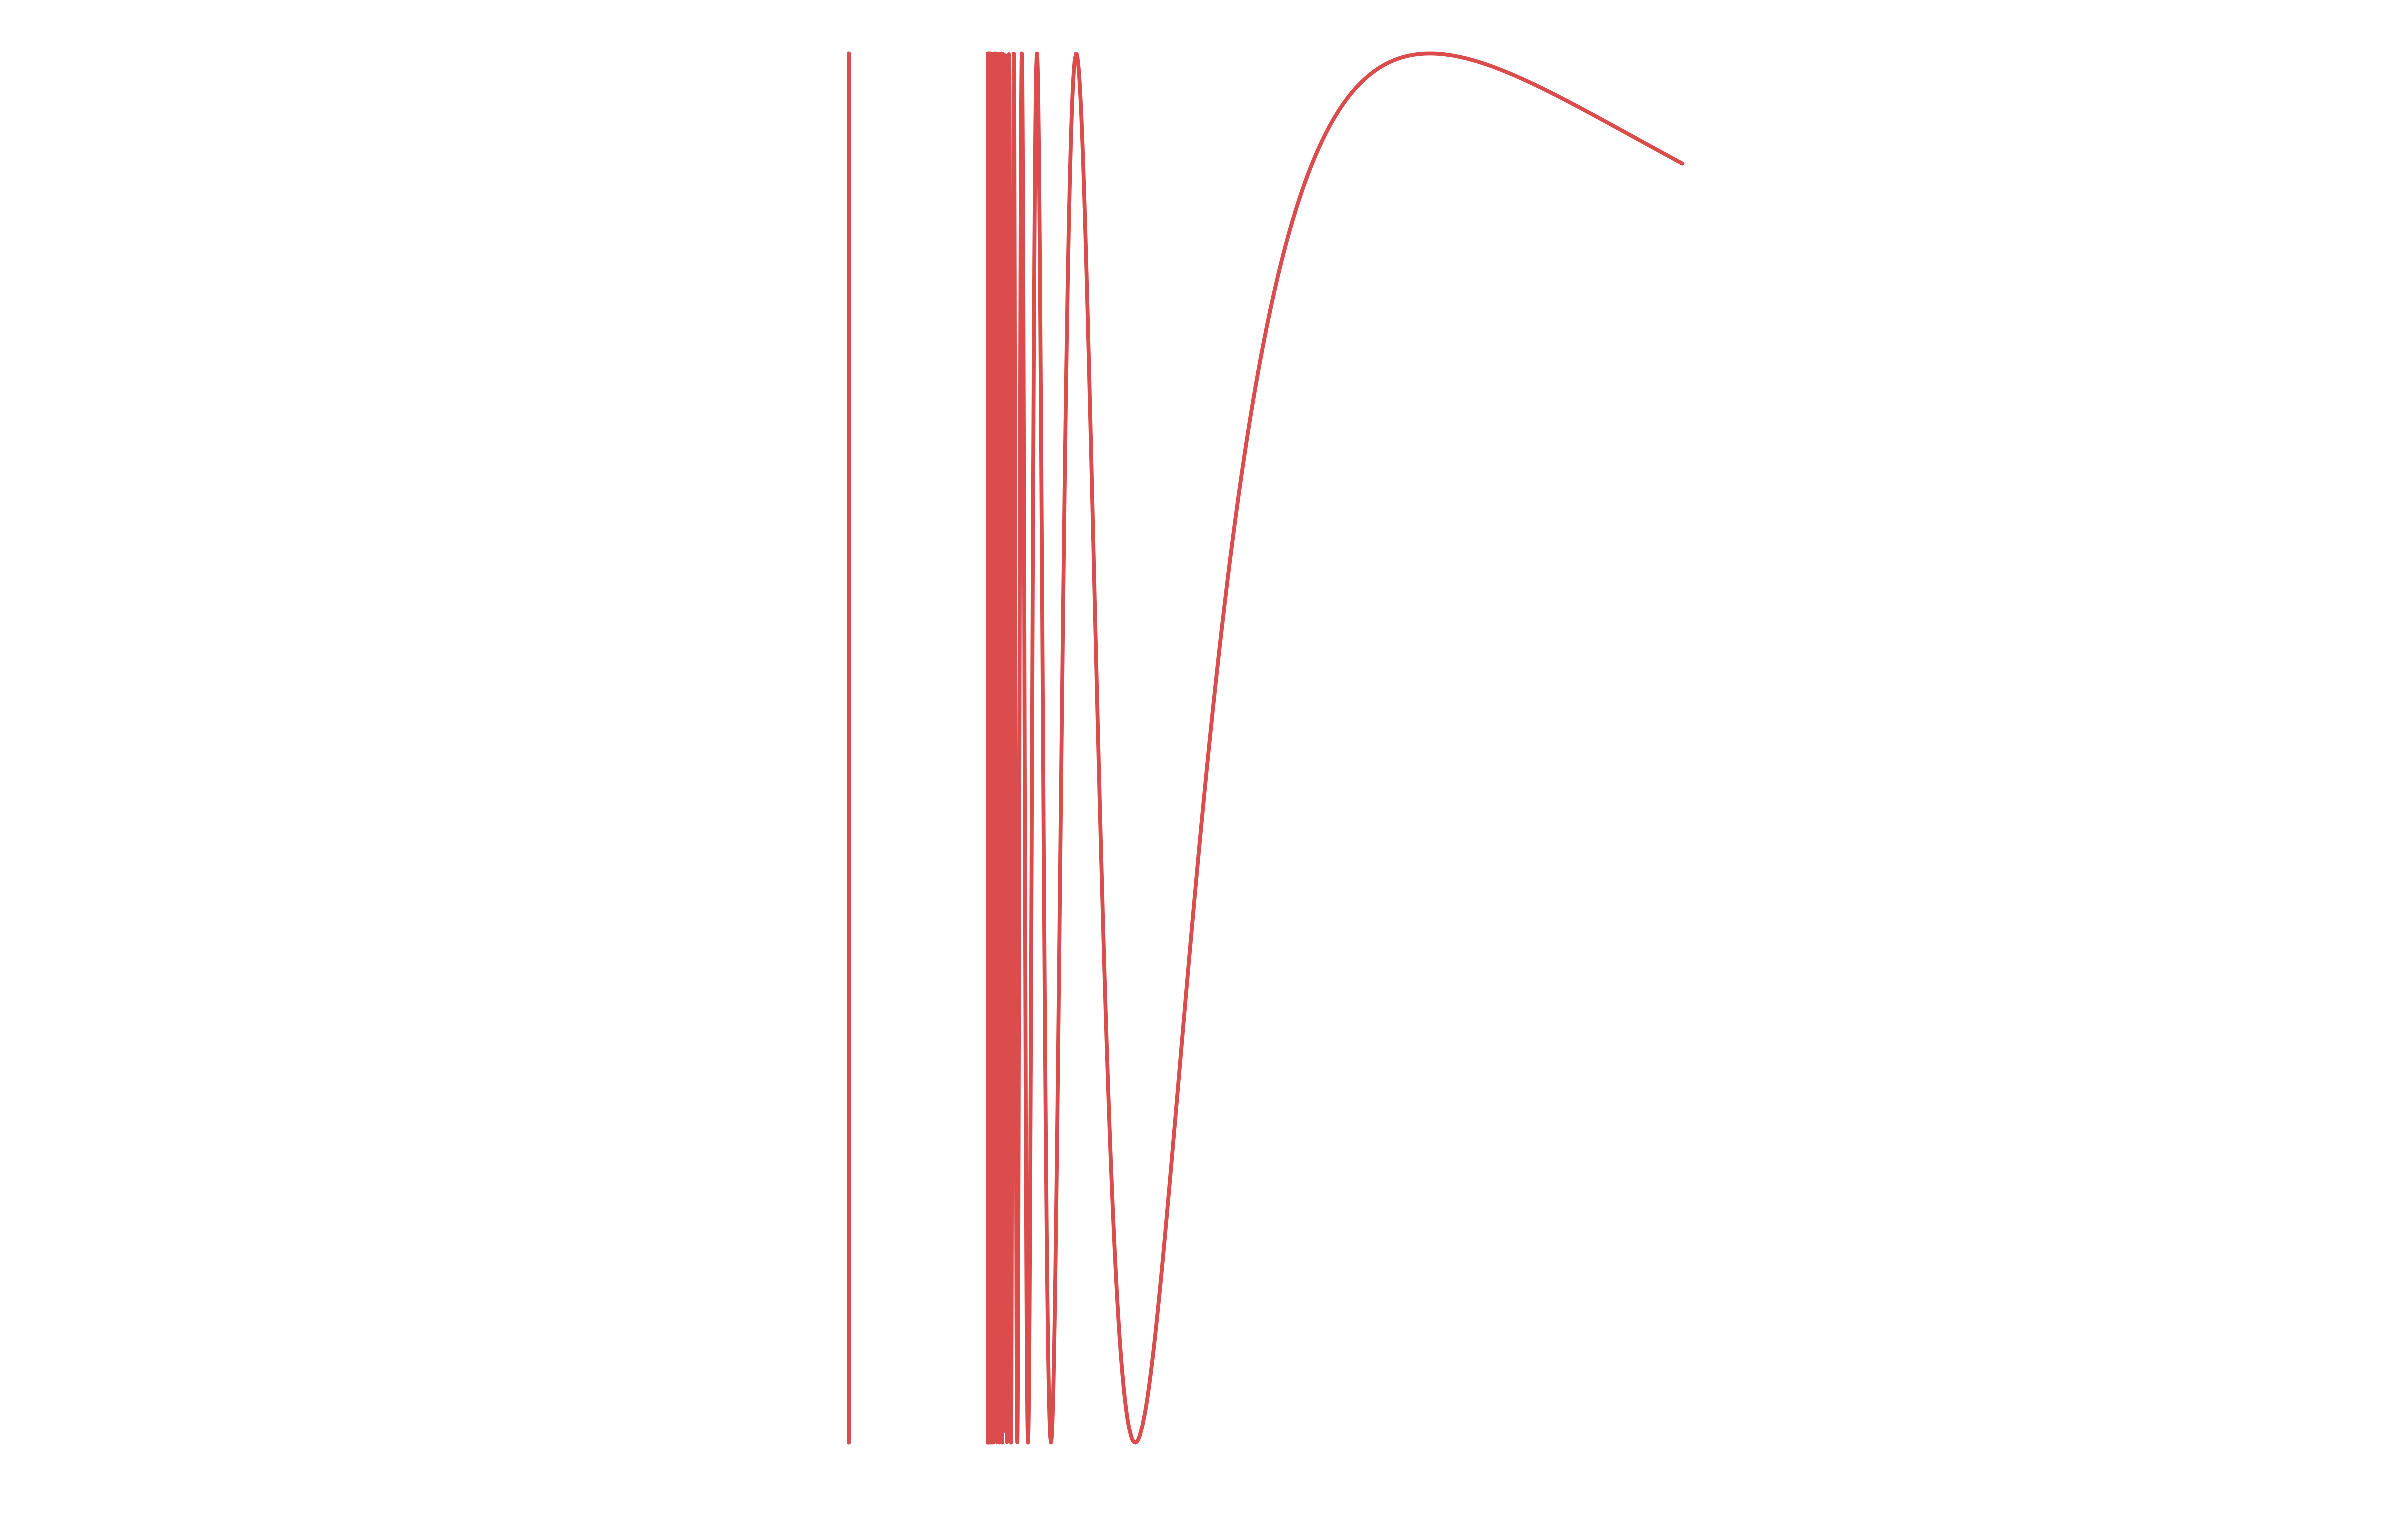
\includegraphics[scale = 0.2]{Figures/Chapter3/topologistsSineCurve.eps}
            \caption{The topologists Sine Curve, defined by $x \times \sin{\frac{1}{x}}$.}
            \label{fig_3.2}
        \end{figure}

        Let $S=\{x \times \sin{\frac{1}{x}}:0 < x \leq 1\}$. This is the image of the continuous map
        $x \rightarrow x \times \sin{\frac{1}{x}$ from $(0,1] \rightarrow \R^2$, Since $(0,1]$ is
            connected, then so is $S$. by theorem \ref{3.1.6}. We call $\cl{S}=S \cup (0 \times
            [-1,1])$ the \textbf{topologist's sine curve} (see figure \ref{fig_3.2}).

            Suppose that $f:[a,c] \rightarrow \cl{S}$ is a path begining at $0$ and ending at a
            point in  $S$. The set  $T=\{t \in \R:f(t) \in 0 \times [-1,1]\}$ is closed, so it has a
            largest element $b$. Then  $f$ is a path mapping  $b \rightarrow 0 \times [-1,1]$ and
            taking all other points to $S$. Suppose that  $[b,c]=[0,1]$ and let $f(t)=(x(t),y(t))$
            where $x(0)=0$, $x(t)>0$ and $y(t)=\sin{\frac{1}{x(t)}}$ for all $t>0$. For  $n \in
            \Z^+$, choose  $0<u<x(\frac{1}{n})$ such that $\sin{\frac{1}{u}}=(-1)^n$. By the
            intermediate value theorem, there are $0<t_n<\frac{1}{n}$ with $x(t_n)=u$. Then the
            sequence $\{t_n\} \rightarrow 0$, and $x(t_n)=(-1)^n$, which diverges; a contradiciton
            since $x(0)=0$ and $\{t_n\} \rightarrow 0$. Hence $\cl{S}$ is not path connected.

    \end{enumerate}
\end{example} 

\section{Outer Measures}

\begin{definition}
    Let $X$ be a set. An \textbf{outer-measure} on $X$ is a function $m^\ast:2^X
    \xrightarrow{} [0, \infty)$ for which the following are true:
    \begin{enumerate}
        \item[(1)] $m^\ast(\emptyset)=0$.

        \item[(2)] If $A \subseteq B$, then $m^\ast(A) \leq m^\ast(B)$.

        \item[(3)] If $\{A_n\}$ is a countable collection of subsets of $X$,
            then
            \begin{equation*}
                m^\ast\Big{(} \bigcup{A_n} \Big{)} \leq \sum{m^\ast(A_n)}
            \end{equation*}
    \end{enumerate}
\end{definition}

\begin{lemma}\label{lemma_1.3.1}
    Let $X$ be a set, and  $\Ec$ a collection of subsets of $X$ for which
    $\emtyset \in \Ec$ and $X \in \Ec$, and let $l:\Ec \xrightarrow{} [0, \infty]$
    a function for which $l(\emptyset)=0$. For any $A \subseteq X$, define
    \begin{equation}\label{equation_1.4}
        m^\ast(A)=\inf{\Big{\{} \sum{l(E_n)} : E_n \in \Ec, \text{ and }
       A \subseteq \bigcup{E_n} \Big{\}}}
    \end{equation}
    Then $m^\ast$ defines an outer-measure.
\end{lemma}
\begin{proof}
    For all $A \subseteq X$, there is a collection $\{E_n\}$ of sets of $\Ec$
    for which $A \subseteq \bigcup{E_n}$. Observe first, that since $l(E_n) \geq
    0$ for all $n$, that  $\sum{l(E_n)} \geq 0$. This makes $m^\ast(A) \geq 0$.
    Now, choose $E_n=\emptyset$ for all  $n$, and we get  $m^\ast(\emptyset)=0$.

    Now, let $A \subseteq B$ subsets of $X$, and let  $\{E_n\}$ a countable
    cover of $B$. Then  $\{E_n\}$ is also a countable cover of $A$. Define then
     $E=\{\sum{l(E_n)} : A \subseteq \bigcup{E_n}\}$ and $F=\{\sum{l(E_n)} :
     B \subseteq \bigcup{E_n}\}$. Since $A \subseteq B$, $F \subseteq E$.
     Therefore, by least upper bounds, we have $\inf{F} \leq \inf{B}$, that is
     $m^\ast(A) \leq m^\ast(B)$.

     Lastly, let $\{A_n\}$ be a countable collection of sets of $X$, and let
     $A=\bigcup{A_n}$. Now, if at least one of the $m(A_n)=\infty$, then we are
     done. Suppose then that $m(A_n)<\infty$ for all $n$. Now, there exists a
     cover of  $A_n$,  $\{E_{n,k}\}_k$ for which
     \begin{equation*}
         \sum_{k}{l(E_{n,k})}<m^\ast(A)+\frac{1}{2^k}
     \end{equation*}
     consider now the countable collection
     $\{E_{n,k}\}_{n,k}=\bigcup_{n}{\{E_{n,k}\}_k}$. Then $\{E_{n,k}\}_{n,k}$ is
     a countable cover for $A$, and we get
     \begin{equation*}
         m^\ast(A) \leq \sum_n{\sum_k{l(E_{n,k})}}<
         \sum_n{m^\ast(A_n)+\frac{1}{2^k}}=\sum_n{m^\ast(A_n)}+\e
     \end{equation*}
     Take then $\e>0$ small, and we get the result.
\end{proof}
\begin{corollary}
    If $E$ is a set of $\Ec$, then $m^\ast(E)=l(E)$.
\end{corollary}
\begin{proof}
    Observe that $E$ covers itself, so that
    $m^\ast(E)=\inf{\{\sum_{i=1}^1{E}\}}=\inf{l(E)}=l(E)$.
\end{proof}

\begin{definition}
    Let $X$ be a set. We call a subset $A$ of  $X$  \textbf{$m^\ast$-measurable}
    if for any subset $E$ of  $X$,
    \begin{equation}\label{equation_1.5}
        m^\ast(E)=m^\ast(E \cap A)+m^\ast(E \cap \com{X}{A})
    \end{equation}
\end{definition}

\begin{lemma}\label{lemma_1.3.2}
    Let $X$ be a set. A subset $A$ of $X$ is  $m^\ast$-measurable if, and only
    if
    \begin{equation*}
        m^\ast(E) \geq m^\ast(E \cap A)+m^\ast(E \cap \com{X}{A}) \text{ for all }
        E \subseteq X
    \end{equation*}
\end{lemma}

\begin{theorem}[Carath\'eodory's Theorem]\label{theorem_1.3.3}
    Let $X$ be a set, and $m^\ast$ an outer-measure on $X$. Then the collection
    of all $m^\ast$-measurable sets forms a  $\s$-algebra. Moreover,  $m^\ast$
    is a complete measure on this $\s$-algebra.
\end{theorem}
\begin{proof}
    Let $\Mc$ be the collection of all  $m^\ast$-measurable sets. Observe first
    that if  $A \in \Mc$, then so is $\com{X}{A}$, by symetry of equation
    \ref{equation_1.5}. So $\Mc$ is closed under complements. Now, let  $A,B \in
    \Mc$. Then we have
    \begin{align*}
        m^\ast(E) &= m^\ast(E \cap A)+m^\ast(E \cap \com{X}{A}) \\
               &= m^\ast(E \cap A \cap B)+m^\ast(E \cap A \cap \com{X}{B})
                        +m^\ast(E \cap B \cap \com{X}{A})+m^\ast(E \cap
                        \com{X}{A} \cap \com{X}{B}) \\
    \end{align*}
    Now, since $A \cup B=(A \cap B) \cup (A \cap \com{X}{B}) \cup (B \cap
    \com{X}{A})$, so by subadditivity, we get
    \begin{equation*}
        m^\ast(E \cap A \cap B)+m^\ast(E \cap A \cap \com{X}{B})+m^\ast(E \cap
        \com{X}{A} \cap B) \geq m^\ast(E \cap (A \cup B))
    \end{equation*}
    i.e. $m^\ast(E) \geq m^\ast(E \cap (A \cup B))+m^\ast(E \cap \com{X}{(A \cup
    B)})$. That is, $A \cup B \in \Mc$, making $\Mc$ an algebra.

    Now, let  $\{A_n\}$ be a countable disjoint collection of
    $m^\ast$-measurable sets, and take  $B_n=\bigcup_{i=1}^n{A_i}$, and take
    $B=\bigcup{B_n}$. Then for all $E \subseteq X$
    \begin{align*}
        m^\ast(E \cap B_n) &= m^\ast(E \cap B_n \cap A_n)+m^\ast(E \cap B_n \cap
                        \com{X}{A_n}) \\
                     &= m^\ast(E \ca A_n)+m^\ast(E \cap B_{n-1})
    \end{align*}
    an induction argument on the collection $\{B_n\}$ gives us
    \begin{equation*}
        m^\ast(E \cap B_n)=\sum_{i=1}^n{m^\ast(E \cap A_i)}
    \end{equation*}
    therefore
    \begin{equation*}
        m^\ast(E)=m^\ast(E \cap B_n)+m^\ast(E \cap \com{X}{B_n}) \geq
        \sum_{i=1}^n{m^\at(E \cap A_i)}+m^\ast(E \cap \com{X}{B_n})
    \end{equation*}
    letting $n \xrightarrow{} \infty$,
    \begin{equation*}
        m^\ast(E) \geq \sum{m^\at(E \cap A_n)}+m^\ast(E \cap \com{X}{B_n})
    \end{equation*}
    so that $B \in \Mc$. Taking $E=B$, we get  $m^\ast(B)=\sum{m^\ast(A_n)}$ so
    that $m^\ast$ is countably additive, and $\Mc$ is a $\s$-algebra.

    Finally, let $m^\ast(A)=0$, then for any $E \subseteq X$, we have
    \begin{equation*}
        m^\ast(E) \leq m^\ast(E \cap A)+m^\ast(E \cap \com{X}{A})=
        m^\ast(E \cap \com{X}{A}) \leq m^\ast(E)
    \end{equation*}
    so that $A \in \Mc$, which makes $m^\ast$ complete on $\Mc$.
\end{proof}

\begin{definition}
    Let $X$ be a set, and  $\Ac$ an algebra on  $X$. We define a
    \textbf{pre-measure} on $\Ac$ to be a function  $m_0:\Ac \xrightarrow{}
    [0,\infty]$ for which
    \begin{enumerate}
        \item[(1)] $m_0(\emptyset)=0$.

        \item[(2)] If $\{A_n\}$ is a countably disjoint collection of sets in
            $\Ac$, for which  $\bigcup{A_n} \in \Ac$, then
            \begin{equation}\label{equation_1.6}
                m_0\Big{(} \bigcup{A_n} \Big{)}=\sum{m_0(A_n)}
            \end{equation}
    \end{enumerate}
\end{definition}

\begin{lemma}\label{lemma_1.3.4}
    Pre-measures on algebras define outer-measures on the overlying sets.
\end{lemma}
\begin{proof}
    Consider the definition of the outer measure $m^\ast$ from equation
    \ref{equation_1.4}, simply take $l=m_0$, and $\Ec=\Ac$.
\end{proof}

\begin{lemma}\label{lemma_1.3.5}
    Let $X$ be a set, and  $\Ac$ an algebra on  $X$. If  $m_0$ is pre-measure on
    $\Ac$, and the measure $m^\ast$ is define by
    \begin{equation*}
        m^\ast(A)=\inf{\Big{\{} \sum{m_0(E_n)} : E_n \in \Ac, \text{ and }
       A \subseteq \bigcup{E_n} \Big{\}}}
    \end{equation*}
    then the following are true.
    \begin{enumerate}
        \item[(1)] $m_0=m^\ast$ on $\Ac$.

        \item[(2)] Every set in $\Ac$ is  $m^\ast$-measurable.
    \end{enumerate}
\end{lemma}
\begin{proof}
    For (1), suppose that $A \in \Ac$, and that $A \subseteq \bigcup{E_n}$ for
    $E_n \in \Ac$. Take
    \begin{equation*}
        F_n=A \cap \com{A_n}{\Big{(} \bigcup_{i=1}^{n-1}{A_i} \Big{)}}
    \end{equation*}
    then $\{F_n\}$ is a disjoint countable collection of sets of $\Ac$ for which
     $A=\bigcup{F_n}$. Hence
     \begin{equation*}
         mo(A)=\sum{m_0(F_n)} \leq \sum{m_0(E_n)}
     \end{equation*}
     it follows from hypothesis that $m_0(A) \leq m^\ast(E)$. For the reverse
     inclusion, simply take $A \subseteq \bigcup{E_n}$ with $A=E_1$ and
     $E_n=\emptyset$ for all  $n>1$.

     For (2), if $A \in \Ac$, and $E \subseteq X$, and $\e>0$, there is a
     collection  $\{B_n\}$ of sets of $\Ac$ with  $A \subseteq \bigcup{B_n}$,
     and
     \begin{equation*}
         \sum{m_0(B_n)}<m^\ast(A)+\e
     \end{equation*}
     by additivity of $m_0$ on $\Ac$, we get
     \begin{equation*}
         m^\ast(E)+\e \geq \sum{m_0(B_n \cap A)}+\sum{m_0(B_n \cap \com{X}{A})}
                    \geq m^\ast(E \cap A)+m^\ast(E \cap \com{X}{A})
     \end{equation*}
\end{proof}

\begin{theorem}\label{theorem_1.3.6}
    Let $X$ be a set, and  $\Ac$ an algerba on  $X$. Let  $m_0$ be a pre-measure
    on $\Ac$, and let  $\Mc$ the  $\s$-algebra generated by  $\Ac$. Then there
    exists a measure  $m$ on  $\Mc$ whose restriction to  $\AC$ is  $m_0$.
    Moreover, if $n$ is another measure extending from $m_0$, then
    \begin{equation*}
        n(E) \leq m(E) \text{ for all } E \in \Mc
    \end{equation*}
    where equality holds when $m(E)<\infty$. Lastly, if $m_0$ is $\s$-finite,
    then  $m$ is the unique extension of  $m_0$ to $\Mc$.
\end{theorem}
\begin{proof}
    Define again,
    \begin{equation*}
        m^\ast(A)=\inf{\Big{\{} \sum{m_0(E_k)} : E_k \in \Ac, \text{ and }
       A \subseteq \bigcup{E_k} \Big{\}}}
    \end{equation*}
    then by Carath\'eodory's theorem, lemma \ref{lemma_1.3.5}, the first result
    follows, since the $\s$-algebra of all  $m^\ast$-measurable sets contains
    $\Ac$, and as consequence, also contains $\Mc$.

    Now, let $E \in \Mc$ with $E \subseteq \bigcup{A_k}$, where $A_k \in \Ac$.
    Then
    \begin{equation*}
        n(E) \leq \sum{n(A_n)}=\sum{m_0(A_n)}
    \end{equation*}
    which gives us $n(E) \leq m(E)$. Now, set $A=\bigcup{A_n}$, and observe that
    \begin{equation*}
        n(A)=\lim_{k \xrightarrow{} \infty}{n\Big{(} \bigcup_{i=1}^k{A_i} \Big{)}}
        =\lim_{k \xrightarrow{} \infty}{m\Big{(} \bigcup_{i=1}^k{A_i}
        \Big{)}}=m(A)
    \end{equation*}
    if $m(E)<\infty$, choose $A_k$ such that  $m(A)<m(E)+\e$ for $\e>0$. Then
    $m(\com{A}{E})<\e$, and
    \begin{equation*}
        m(E) \leq m(A)=n(A)=n(E)+n(\com{A}{E}) \leq n(E)+m(\com{A}{E}) \leq
        n(E)+\e
    \end{equation*}
    taking $\e$ small, we get $n(E)=m(E)$.

    Finally, suppose that $m_0$ is $\s$-finite, and let $X=\bigcup{A_k}$ for
    s me0disjoint collection $\ A_n\}$, then $ m_0 m_0)<\infty$. Then for every
    $E \in \Mc$,
    \begin{equation*}
        m(E)=\sum{m(E \cap A_k)}=\sum{n(E \cap A_k)}=n(E)
    \end{equation*}
    so that $m=n$, making $m$ unique.
\end{proof}

\section{Roots of Analytic Functions}

%----------------------------------------------------------------------------------------
%	SECTION 1.1
%----------------------------------------------------------------------------------------

\section{Rectifiable Curves.}

\begin{definition}
    We call a continuous mapping $\gamma:[a,b] \rightarrow \R^k$ a
    \textbf{curve} in $\R^k$, on  an interval $[a,b]$. If  $\gamma$ is 1-1, we
    call the curve an \textbf{arc}, and we call  $\gamma$ a \textbf{closed
    curve} if  $\gamma(a)=\gamma(b)$.

    Now, for each partition $P$ of  $[a,b]$, and for  $\gamma$ a curve on
    $[a,b]$, and let:
        \begin{equation}
            \Lambda(\gamma,P)=\sum_{i=1}^{n}{||\gamma(x_i)-\gamma(x_{i-1})||}		
        \end{equation}
    We deefine the \textbf{length} of $\gamma$ to be :
        \begin{equation}
            \Lambda(\gamma)=\sup_{P}{\Lambda(\gamma,P)}		
        \end{equation} 
        If $\gamma$ is of finite length  (i.e. $\Lambda(\gamma)<\infty$), then
        we call $\gamma$ a \textbf{rectifiable} curve.
\end{definition}

\begin{theorem}\label{7.5.1}
    Let $\gamma$ be a differentiable curve on  $[a,b]$, if  $\gamma'$ is
    continuous, then  $\gamma$ is rectifiable and
        \begin{equation}
            \Lambda(\gamma)=\int_{a}^{b}{||\gamma'|| dt}		
        \end{equation} 
\end{theorem}
\begin{proof}
    If $a \leq x_{i-1}<x_i \leq b$, then
    $||\gamma(x_i)-\gamma(x_{i-1})||=||\int_{x_{i-1}}^{x_i}{\gamma' dt}|| \leq
    \int_{x_{i-1}}^{x_i}{||\gamma'|| dt}$, by the Fundamental theorem of
    calculus, thus $\Lambda(\gamma,P) \leq \int_{a}^{b}{||\gamma'|| dt}$ 
    for every partition $P$ of  $[a,b]$, then cinsequently, we have
    $\Lambda(\gamma)=\int{||\gamma'|| dt}$. Consequently, $\gamma$ is
    rectifiable.

    Now let  $\epsilon>0$, since  $\gamma'$ is uniformly continuous on  $[a,b]$,
    there is a  $\delta>0$ such that  $||\gamma'(s)-\gamma'(t)||<\epsilon$
    whenever  $|s-y|<\delta$ for  $s,t \in [a,b]$. Let $P$ be a partition of
    $[a,b]$, with  $\Delta{x_i}<\delta$ for all  $i$, and it  $x_{i-1} \leq t
    \leq x_i$, we have  $||\gamma'(t)|| \leq ||\gamma'(x_i)||+\epsilon$, hence:
        \begin{align*}
            \int_{x_{i-1}}^{x_i}{||\gamma'||\Delta{x_i}} &\leq ||\gamma'(x_i)||\Delta{x_i}+\epsilon\Delta{x_i} \\ 
                &= ||\int_{x_{i-1}}^{x_i}{(\gamma'(t)+\gamma'(x_i)-\gamma'(t))}||+\epsilon\Delta{x_i} \\
                &\leq ||\int_{x_{i-1}}^{x_i}{\gamma' dt}||+||\int_{x_{i-1}}^{x_i}{(\gamma'(x_i)-\gamma'(t)) dt}||+\epsilon\Delta{x_i} \\
                & \leq ||\gamma(x_i)-\gamma(x_{i-1})||+2\epsilon\Delta{x_i} \\
        \end{align*}
    Thus, $\int_{a}^{b}{||\gamma'|| dt} \leq \Lambda(\gamma,P)+2\epsilon(b-a)$, 
    so for  $\epsilon$ small enough, we get that  $\int{||\gamma'||} \leq \Lambda(\gamma)$.
\end{proof}

\section{Gr\"obner Bases}
\label{section_7.6}

\begin{definition}
  Let $R$ be a Noetherian ring, and $\leq$ a monomial ordering on
  $R[x_1, \dots, x_n]$. We define the \textbf{leading term} of a
  polynomial $f(x_1, \dots, x_n)$ to be the maximum element of the
  ideal $(f)$, and denote it $LT(f)$. If $\af$ is an ideal in $R[x_1,
  \dots, x_n]$, then we define the \textbf{ideal of leading terms} of
  $\af$ to be the ideal generated by all leading terms of polynomials
  of $\af$; i.e.
  \begin{equation*}
    LT(\af)=(LT(f) : f \in \af)
  \end{equation*}
  If $\af=(f_1, \dots, f_m)$, we write $LT(f_1, \dots, f_m)$. If
  $\af=(f)$, we keep the previous convention $LT(\af)$.
\end{definition}

\begin{definition}
  Let $f(x_1, \dots, x_n)$ a multi-variate polynomial over a
  Noetherian ring. We define the \textbf{multi-degree} of $f$ to be
  the multi-degree of $LT(f)$, and we denote it $\partial{f}$.
\end{definition}

\begin{proposition}\label{proposition_7.6.1}
  Let $f_1, \dots, f_m$ be multivariate polynomials over a Noetherian
  ring. Then
  \begin{equation*}
    (LT(f_1), \dots, LT(f_m)) \subseteq LT(f_1, \dots, f_m)
  \end{equation*}
\end{proposition}
\begin{proof}
  Observe that since $f_i \in \af$ for each $1 \leq i \leq m$, then
  $LT(f_i) \in LT(\af)$ for each $1 \leq i \leq m$.
\end{proof}

\begin{proposition}\label{proposition_7.6.2}
  Let $k$ be field, and $f,g \in k[x_1, \dots, x_n]$. Then
  the following are true:
  \begin{enumerate}
    \item[(1)] $LT(fg)=LT(f)LT(g)$.

    \item[(2)] $LT(f+g) \leq \max{\{LT(f), LT(g)\}}$ with equality
      holding if $LT(f) \neq LT(g)$.
  \end{enumerate}
\end{proposition}
\begin{proof}
  Let $AX^\a=LT(f)$ and $BX^\b=LT(g)$, and make the convention $f(x_1,
  \dots, x_n)=f(X)$. Then we have for some $h,h' \in R[x_1, \dots,
  x_n]$ that $f(X)=AX^\a+h(X)$ and $g=BX^\b+h'(X)$. Then
  \begin{align*}
    fg(X) &=  (AX^\a+h(X))(BX^\b+h'(X))  \\
          &= (AB)X^\a X^\b+(AX^\a h'(X)+BX^\b h(X)+h(X)h'(X))  \\
          &=  (AB)X^{\a+\b}+h''(X)  \\
  \end{align*}
  so that $LT(fg)=LT(f)LT(g)$.

  Now, we also observe that
  \begin{equation*}
    f+g(X)=(AX^\a+BX^\b)+(h(X)+h'(X))
  \end{equation*}
  if $\a=\b$, and $B=-A$, then $f+g(X)=h(X)+h'(X)$ and $LT(f+g)<AX^\a$
  and $LT(f+g)<BX^\b$, so that $LT(f+g)<\max{\{AX^\a,BX^\b\}}$. Now, we have
  if  $\a \neq \b$, then
  \begin{align*}
    f+g(X)=AX^\a+(BX^\b+h(X)+h'(X))  & \text{ if } \b < \a  \\
    f+g(X)=AX^\b+(BX^\a+h(X)+h'(X))  & \text{ if } \a < \b  \\
  \end{align*}
  in either case either $LT(f+g)=\max{\{X^\a,X^\b\}}$.
\end{proof}
\begin{corollary}
  The following are true:
  \begin{enumerate}
    \item[(1)] $\partial{(fg)}=\partial{f}+\partial{g}$.

    \item[(2)] $\partial{(f+g)} \leq \max{\{\partial{f},
      \partial{g}\}}$, with equality holding if $\partial{f} \neq
      \partial{g}$.
  \end{enumerate}
\end{corollary}

\begin{proposition}\label{proposition_7.6.3}
  Let $R$ be a Noetherian ring. Let $\af=(X^{\a_1}, \dots, X^{\a_m})$ in $R[x_1,
  \dots x_n]$ and ideal and $f \in R[x_1, \dots, x_n]$. Then $f \in
  \af$ if, and only if each monomial term of $f$ is a multiple of some
  monomial  $X^\a_i$ generating $\af$.
\end{proposition}
\begin{proof}
  Suppose that $f \in \af$. Then
  \begin{equation*}
    f(x_1, \dots, x_n)=f(X)=\sum_{i=1}^m{A_mX^{\a_i}}
  \end{equation*}
  and notice that each monomial $X^{\a_i}$ is a multiple of itself.

  Conversely suppose that
  \begin{equation*}
    f(X)=\sum_{j=1}^n{A_jX^{\b_j}}
  \end{equation*}
  and that there is an $X^{\a_i}$ for which $X^{\a_i}|X^{\b_j}$ for
  all $1 \leq j \leq n$. Then $X^{\b_j} \in (X^{\a_i}) \subseteq
  (X^{\a_1}, \dots, X^{\a_m})$. Then $f \in \af$.
\end{proof}

\begin{example}\label{example_7.8}
  Let $k$ be a field.
  \begin{enumerate}
    \item[(1)] Choose the lexicographic order $x>y$ on $k[x,y]$. Let
      $f(x,y)=x^3y-xy^2+1$ and $g(x,y)=-y^3+x^2y^2-1$. Then
      $LT(f)=x^3y$ with $\partial{f}=(3,1)$, and $LT(g)=x^2y^2$ with
      $\partial{g}=(2,2)$. Then
      \begin{align*}
        LT(fg)=x^5y^3 & \text{ and } \partial{(fg)}=(5,3) \\
        LT(f+g)=x^3y  & \text{ and } \partial{(f+g)}=(3,0)  \\
      \end{align*}
      Now, take $\af=(f,g)$, then $(x^3y,x^2y^2) \subseteq LT(f,g)$.
      However, observe that $yf(x,y)-xg(x,y)=x+y \in \af$, and
      $LT(yf+xg)=x \in LT(f,g)$. However $x \notin
      (x^3y,x^2y^2)$. That is, in general, if $\af=(f_1,
      \dots, f_m)$, then $LT(f_1, \dots, f_m) \neq (LT(f_1), \dots
      LT(f_m))$.

    \item[(2)] Choose the lexicographic ordering $y>x$ in  $k[x,y]$.
      Let again $f(x,y)=x^3y-xy^2+1$ and $g(x,y)=-y^3+x^2y^2-1$. Then
      $LT(f)=xy^2$ with $\partial{f}=(1,2)$ and $LT(g)=y^3$ with
      $\partial{g}=(0,3)$. Then
      \begin{align*}
        LT(fg)=xy^5 & \text{ and } \partial{(fg)}=(1,5) \\
        LT(f+g)=-y^3 & \text{ and } \partial{(f+g)}=(03) \\
      \end{align*}
      Again, we have $(xy^2, y^3) \subseteq LT(f,g)$, but $LT(f,g)
      \neq (xy^2,y^3)$. We observe that $y \in LT(f,g)$ but $y \notin
      (xy^2,y^3)$.

    \item[(3)] Choose any order on $k[x,y]$, and let $f(x,y) \neq 0$.
      Let $\af=(f)$, then $LT(\af)=(LT(f))$, since every monomial term
      of $f$ is a multiple of  $LT(f)$.
  \end{enumerate}
\end{example}

\begin{definition}
  Let $k$ be a field, and $\af$ an ideal of $k[x_1, \dots, x_n]$. We
  call a finite set of generators $G=\{g_1, \dots, g_m\}$ of $\af$ a
  \textbf{Gr\"obner basis} for $\af$ if
  \begin{equation*}
    LT(\af)=(LT(g_1), \dots, LT(g_m))
  \end{equation*}
\end{definition}

\section{Cyclotomic Polynomials}
\label{section_8.7}

\begin{definition}
  We define \textbf{Euler's totient} to be the map $\phi:\Z \xrightarrow{} \Z$
  defined by the rule $\phi(n)=|\{a \in \Z : (a,n)=1\}|$. That is, $\phi$
  of  $n$ is the number of all integers less than  $n$, coprime to  $n$.
\end{definition}

\begin{definition}
  We define $\Xi_n$ to be the \textbf{group of all primitive $n$-th roots of
  unity}, $\xi$ for which  $\xi^n=1$.
\end{definition}

\begin{lemma}\label{lemma_8.7.1}
  $\Xi_n \simeq \faktor{\Z}{n\Z}$.
\end{lemma}
\begin{proof}
  The map $a \xrightarrow{} \xi^a$ defines the required isomorphism.
\end{proof}
\begin{corollary}
  $\ord{\Xi_n}=\phi(n)$ where $\phi$ is Euler's totient.
\end{corollary}
\begin{proof}
  Since $\xi^n \equiv \xi^{0 \mod{n}} \equiv 1$, we have every non identity
  power of $\xi$ has exponenct coprime to  $n$. That is there are $\phi(n)$
  such distinct powers of$\xi$.
\end{proof}
\begin{corollary}
  If $d|n$, then  $\Xi_d \leq \Xi_n$.
\end{corollary}
\begin{proof}
  Notice that if $d|n$, then $d=mn$ for some  $m \in \Z^+$. Then $\xi^d=1$
  implies  $(\xi^d)=\xi^{dm}=\xi^n=1$.
\end{proof}

\begin{definition}
  We define the \textbf{$n$-th cyclotomic polynomial} to be the polynomial
  \begin{equation*}
    \Phi_n(x)=\prod{x-\xi}
  \end{equation*}
  having as roots all $n$-primitive roots of unity.
\end{definition}

\begin{lemma}\label{lemma_8.7.2}
  The $n$-th cyclotomic polynomial  $\Phi_n$ has degree
  $\deg{\Phi_n}=\phi(n)$, where $\phi$ is Euler's totient.
\end{lemma}
\begin{proof}
  Recall that $\ord{\Xi_n}=\phi(n)$, and since the elements of $\Xi_n$ are the
  roots of  $\Phi_n$, there are  $\phi(n)$ such roots. This puts
  $\deg{\Phi_n}=\phi(n)$.
\end{proof}

\begin{example}[Computing Cyclotomic Polynomials]\label{8.18}
  Recall that the polynomial $x^n-1$ has as roots precisely all  $n$-th roots
  of unity  $\xi$, that is $\xi^n=1$. If $x^n-1 \in F[x]$, $F$ a field, the
  the splitting field of  $x^n-1$ is  $F(\xi)$. Then we have
  \begin{equation*}
    x^n-1=\prod_{\xi \in \Xi_n}{(x-\xi)}
  \end{equation*}
  Now, grouping those factors where $\xi^d=1$ for some  $d|n$, then we have
  \begin{equation*}
    x^n-1=\prod_{\xi \in \Xi_d}{(x-\xi)}\prod_{\xi \in \Xi_n}{(x-\xi)}=
    \prod{d|n}{\prod_{\xi \in \Xi_n}{(x-\xi)}}=\prod_{d|n}{\Phi_n(x)}
  \end{equation*}
  that is,
  \begin{equation*}
    x^n-1=\prod_{d|n}{\Phi_d(x)}
  \end{equation*}
  which gives a method for computing $\Phi_n$ recursively.

  We have  $\Phi_1(x)=x-1$ and $\Phi_2(x)=x+1$. Now,
  $\Phi_3(x)=\Phi_1(x)\Phi_3(x)=(x-1)\Phi_3(x)$, so that
  \begin{equation*}
    Phi_n(x)=x^2+x+1
  \end{equation*}
  We have
  $\Phi_4(x)=\Phi_1(x)\Phi_2(x)\Phi_4(x)=(x-1)(x+1)\Phi_4(x)=(x^2-1)\Phi_4(x)$.
  So
  \begin{equation*}
    \Phi_4(x)=x^2+1
  \end{equation*}
  Similarly,
  \begin{align*}
    \Phi_5(x)   &=  x^4+x^3+x+1 \\
    \Phi_6(x)   &=  x^2-x+1 \\
    \Phi_7(x)   &=  x^6+x^5+x^4+x^3+x^2+x+1 \\
    \Phi_8(x)   &= x^4+1    \\
    \Phi_9(x)   &=  x^6+x^x+1   \\
    \Phi_{10}(x)   &=   x^4-x^3+x^2-x+1 \\
    \Phi_{11}(x)   &=   x^{10}+x^9+x^8+x^7+x^6+x^5+x^4+x^3+x^2+x+1  \\
    \Phi_{12}(x)   &=   x^4-x^2+1   \\
  \end{align*}
  Also observe that if $p$ is prime, then
  \begin{equation*}
    \Phi_p(x)=\sum_{i=0}^{p-1}{x^i}=x^{p-1}+x^p+\dots+x+1
  \end{equation*}
\end{example}

\begin{lemma}\label{lemma_8.7.3}
  $\Phi_n(x)$ is monic over $\Z$.
\end{lemma}
\begin{proof}
  Notice that since $x^n-1=\prod{\Phi_d(x)}$, is monic, then each $\Phi_d$
  must also be monic for all  $d|n$.

  Now, by induction on $n$, for  $n=1$, it is clear that  $x-1$ has
  coefficiencts in  $\Z$  (if $x^n-1 \in \Z[x]$ we are done, if not, just take
  $1_F \xrightarrow{} 1_\Z$, whre $F$ is the underlying field of  $x^n-1$).
  Now, suppose that $\Phi_d(x) \in \Z[x]$ for all $1 \leq d <n$, and  $d|n$.
  Then  $x^n-1=f(x)\Phi_n(x)$, where $f(x)=\prod{\Phi_d(x)}$ is monic over
  $\Z$. Moreover,  $f|x^n-1$, in the splitting field $\Q(\xi)$ (since we take
  $1_F \xrightarrow{} F_\Z$), where $\xi^n=1$. Then  $f|x^n-1$ over  $\Q$ by
  the division theorem, and by Gauss' lemma, $f|x^n-1$ in $\Z$. So $\Phi_n \in
  \Z[x]$.
\end{proof}

\begin{theorem}\label{lemma_8.7.4}
  $\Phi_n$ is irreducible over  $\Z$.
\end{theorem}
\begin{proof}
  Again, if $x^n-1 \in F[x]$ for some field $F$, take  $1_F \xrightarrow{}
  1_\Z$ so that $x^n-1 \in \Z[x]$. Suppose then that $\Phi_n(x)=f(x)g(x)$
  where $f$ and  $g$ are monic, and  $f$ is irreducible. Let $\xi^n=1$, a
  primitive $n$-th root, so that $\xi$ is a root of $f$. Then $f$ is the
  minimal polynomial for $\xi$ over  $\Q$. Now, let $p$ a prime such that $p
  \nmid n$. Then $\xi^p$ is a $n$-th root, of $f$ or $g$. If  $f(\xi^p)=0$,
  then for all $a$ with  $(a,n)=1$, we have $\xi^a$ is a root of $f$.
  Moreover,  $a=p_1 \dots p_k$ where each $p_i \nmid n$ is prime. That means
  tht  $\xi^{p_1}$, $(\xi^{p_1})^{p_2}, \dots, \xi^n$ are all roots of $f$
  making  $f=\Phi_n$ and we are done.

  Suppose then that $g(\xi^p)=0$. Then $\xi$ is root of  $g(x^p)$,
  and since $f$ is minimal, $f|g(x^p)$ in $\Z[x]$. Then we have
  $g(x^p)=f(x)h(x)$ for $f,h \in \Z[x]$. reducing mod $p$, we get
  $g(x^p) \equiv f(x)h(x) \mod{p}$ in $\F_p[x]$; but $g(x^p) \equiv (g(x))^p
  \mod{p}$. Since $\F_p[x]$ is a unique factorization domain, we get that $f
  \mod{p}$ and $g \mod{p}$ have a common factor. Then $\Phi_n(x) \equiv
  f(x)g(x) \mod{p}$ has a multiple root in $\F_p[x]$ ; implying that $x^n-1$
  has a multiple root, which is impossible; since $x^n-1$ has  $n$ distinct
  roots. Therefore $\xi^p$ is a root of  $f$.
\end{proof}
\begin{corollary}
  $[\Q(\xi):\Q]=\phi(n)$.
\end{corollary}
\begin{proof}
  We have by above that $\Phi_n$ is the minimal polynomial for  $\xi$ over
  $\Q$.
\end{proof}

\begin{example}\label{8.19}
  Let $\xi^8=1$ an  $8$-th root of unity. Then  $[\Q(\xi):\Q]=4$ and $\Q(\xi)$
  has minimal polynomial $\Phi_8(x)=x^4+1$. Moreover, $\Q(\xi)$ contains a
  primitive $4$-th root of unity $i^4=1$ (over $\C$,  $i^2=-1$). So that
  $\Q(i) \subseteq \Q(\xi)$. We als get that $\xi+\xi^7=\sqrt[]{2}$ (since
  $\xi=e^{\frac{2i\pi}{8}}$ over $\C$), and $\Q(\xi)=\Q(i,\sqrt[]{2})$.
\end{example}

\section{Lattices and Flats of A Matroid.}

\section{Integral Elements}\label{section_1.9}

\section{Field Extensions}\label{section_1.10}

\section{Extensions and Contractions of Ideals}

For this section, $A$ and  $B$ denote commutative rings with identity.

\begin{definition}
  Let $f:A \xrightarrow{} B$ a ring homomorphism. The extension of the ideal
  $\af$ in $A$ is the ideal $\af^\e$ generated by $f(\af)$ in $B$. That is,
  $\af^e=Bf(\af)$.
\end{definition}

\begin{lemma}\label{1.10.1}
    Let $f:A \xrightarrow{} B$ a ring homomorphism and $\af$ an ideal of $A$.
    Then
    \begin{equation*}
        \af^e=\{\sum{y_if(x_i) : y_i \in B \text{ and } x_i \in \af}\}
    \end{equation*}
\end{lemma}
\begin{proof}
    This follows directly from the definition of $\af^e$.
\end{proof}

\begin{definition}
    Let $f:A \xrightarrow{} B$ a ring homomorphism. We define the
    \textbf{contraction} of the ideal $\bf$ of  $\bf$ to be the preimage
    $\inv{f}(\bf)$, and denote it $\bf^c$; that is,  $\bf^c=\inv{f}(\bf)$.
\end{definition}

\begin{lemma}\label{1.10.2}
    Let $f:A \xrightarrow{} B$ a ring homomorphism, and $\bf$ and ideal of
    $\bf$. Then $\bf$ is an ideal of $A$. Moreover, if $\bf$ is prime in $B$,
    then  $\bf^c$ is prime in $A$.
\end{lemma}
\begin{proof}
    Let $x \in \bf^c$. Then  $f(x) \in \bf$, so that $-f(x)=\pji(-x) \in
    \bf$, which puts $-x \in \bf^c$; similarly, we get $x+y \in \bf^c$ whenever
    $x,y \in \bf^c$. Lastly, notice that if  $a \in A$, and  $x \in \bf^c$, then
     $f(a)f(x)=f(ax) \in \bf$, so that $\bf^c$ is an ideal.

     Now, suppose that  $\bf$ is prime. Then since  $\bf \neq (1_B)$, $\bf^c
     \neq (1_A)$. Now, let $ab \in \bf^c$. Then  $f(ab)=f(a)f(b) \in
     \bf$. Since $\bf$ is prime, this puts  $f(a) \in \bf$ or $f(b) \in
     \bf$; that is, $a \in \bf^c$ or  $b \in \bf^c$. Therefore, $\bf^c$ must
     also be prime.
\end{proof}

\begin{example}\label{example_1.16}
    Let $f:A \xrightarrow{} B$ a ring homomorphism. We have that for any prime
    ideal $\bf$ of $B$, $\bf^c$ is prime. The same is not true for extensions.
    If $\af$ is prime in $A$,  $\af^e=Bf(\af)$ need not be prime in $B$.
\end{example}

\begin{lemma}\label{1.10.3}
    Let $f:A \xrightarrow{} B$ be a ring homomorphism, with $f=\i \circ \pi$,
    where  $\pi$ is onto and  $\i$ is 1--1. Then there exists a 1--1
    correspondece between the ideals $f(A)$ and the ideals of $A$ containing
     $\ker{f}$. Moreover, prime ideals correspond to prime ideals.
     \[\begin{tikzcd}
        A \\
        {f(A)} & B
        \arrow["\pi"', from=1-1, to=2-1]
        \arrow["\iota"', from=2-1, to=2-2]
        \arrow["{f=\iota \circ \pi}", from=1-1, to=2-2]
      \end{tikzcd}\]
\end{lemma}

\begin{example}\label{example_1.17}
    Consider the map $\Z \xrightarrow{} \Z[i]$ where $i^2=-1$. A prime ideal
    $(p)=p\Z$ may or may not be prime when extended to $\Z[i]$. Now, $\Z[i]$ is
        a PID, so that we have the following.
        \begin{enumerate}
            \item[(1)] $(2)^e=((1+i)^2)$ in $\Z[i]$; that is, it is the square
                of a prime ideal in $\Z[i]$.

            \item[(2)] If $p \equiv 1 \mod{4}$, then $(p^e)$ is the product of
                two prime ideals in $\Z[i]$, and if $p \equiv 3 \mod{4}$,
                $(p)^e$ is a prime ideal in $\Z[i]$.
        \end{enumerate}
\end{example}

\begin{lemma}\label{1.10.4}
    Let $f:A \xrightarrow{} B$ be a ring homomorphism. Then the following are
    true for ideals $\af$ and  $\bf$ of  $A$ and  $B$, respectively.
    \begin{enumerate}
        \item[(1)] $\af \subseteq \af^{ec}$ and $\bf^{ce} \subseteq \bf$.

        \item[(2)] $\af^e=\af^{ece}$, and $\bf^c=\bf^{cec}$.

        \item[(3)] If $C$ is the set of all contracted ideals in $A$, and  $E$
            is the set of all extended ideals in  $B$, then
            \begin{equation*}
                C=\{\af \subseteq A : \af=\af^{ec}\} \text{ and }
                E=\{\bf \subseteq B : \bf=\bf^{ce}\}
            \end{equation*}
            Moreover, there exists a 1--1 correspondence of $C$ onto $E$  given
            by the map $\af \xrightarrow{} \af^e$.
    \end{enumerate}
\end{lemma}
\begin{proof}
    First, consider $\af$ in  $A$. Then  $\af^e=Bf(\af)$, so that if $x \in
    \af$, then  $f(x) \in f(\af)$, that is $x \in \af^{ec}$. Similarly, we
    get $\bf^{ce} \subseteq \bf$.

    Now, for the second assertion, we have
    \begin{equation*}
        (\bf^{ce})^c \subseteq \bf^c \subseteq (\bf^c)^{ec}
    \end{equation*}
    so that $\bf^c=\bf^{cec}$. Similarly, we get $\af^e=\af^{ece}$.

    Finally, let $\af \in C$. Then there is a $\bf$ in $B$ for which
    $\af=\bf^c$. Then  $\af^e=\bf^{ce}=\bf^{cec}=\af^{ec}$. Conversely, if
    $\af=\af^{ec}$, then $\af$ is the contraction of $\af^e$. We use a similar
    argument to prove the result for $E$.
\end{proof}

\begin{lemma}\label{1.10.5}
    If $\af_1,\af_2$ are ideals of $A$ and  $\bf_1,\bf_2$ are ideals of $B$,
    then the following are true.
    \begin{enumerate}
        \item[(1)] $(\af_1+\af_2)^e=\af_1^e+\af_2^e$ and $\bf_1^c+\bf_2^c
            \subseteq (\bf_1+\bf_2)^c$.

        \item[(2)] $(\af_1 \cap \af_2)^e \subseteq \af_1^e \cap \af_2^e$ and
            $\bf_1^c \cap \bf_2^c=(\bf_1 \cap \bf_2)^c$.

        \item[(3)] $(\af_1\af_2)^e=\af_1^e\af_2^e$ and $\bf_1^c\bf_2^c
            \subseteq (\bf_1\bf_2)^c$.

        \item[(4)] $(\af_1:\af_2)^e \subseteq (\af_1^e:\af_2^e)$ and
            $(\bf_1:\bf_2)^c=(\bf_1^c:\bf_2^c)$.

        \item[(5)] $(\sqrt{\af})^e \subseteq \sqrt{\af^e}$ and
            $(\sqrt{\bf})^c=\sqrt{\bf^c}$.
    \end{enumerate}
\end{lemma}
\begin{corollary}
  Let $C$ be the set of all contracted ideals and $E$ the set of all extended
  ideals. Then $C$ is closed under the ideal operations of intersections,
  quotient, and radicals, and  $E$ is closed under the ideal operations of
  addition and products.
\end{corollary}
\begin{proof}
  Let $\af,\bf \in C$, then $(\af \cap \bf)^{ec} \subseteq (\af^e \cap
  \bf^e)^c=(\af^{ec} \cap \bf^{ec})=(\af \cap \bf) \subseteq (a \cap b)^{\ec}$;
  and $(\sqrt{\af})^{ec} \subseteq (\sqrt{\af^e})^c=\sqrt{\af^{ec}} \subseteq
  \sqrt{\af} \subseteq (\sqrt{\af})^{ec}$. Finally, $(\af:\bf) \subseteq
  (\af:\bf)^{ec} \subseteq (\af^{ec}:\bf^{ec})=(\af:\bf)$.

  Now, let $\af, \bf \in E$. Then $\af+\bf=\af^{ce}+\bf^{ce}=(\af^c+\bf^c)^e
  \subseteq (\af+\bf)^{ce} \subseteq \af+\bf$. Likewise, we get the same result
  for $\af\bf$ using the same sequence of operations.
\end{proof}

\section{Noetherian Rings}

\begin{definition}
    Let $A$ be a commutative ring with identity. We say a sequence of ideals
    $\{\af_n\}$ is an \textbf{ascending chain} of ideals if $\af_n \subseteq
    \af_{n+1}$ for all $n \in \Z^+$. We say that the chain  $\{\af_n\}$
    \textbf{stabalizes} if there exists some $k \geq n$, $\af_k=\af_n$.
\end{definition}

\begin{definition}
    Let $A$ be a commutative ring with identity. We call $A$ \textbf{Noetherian}
    if every ascending chain of ideals of $A$ stabalizes. We say that $A$
    satisfies the \textbf{ascending chain condition} on ideals.
\end{definition}

\begin{lemma}\label{1.12.1}
    If $\af$ is an ideal of a Noetherian ring  $A$, then the factor ring
    $\faktor{A}{\af}$ is also Noethrian. In particular, the image of a Noetherian
    ring under any ring homomorphism is Noetherian.
\end{lemma}
\begin{proof}
    This follows by the isomorphism theorems for ring homomorphisms.
\end{proof}

\begin{theorem}\label{1.12.2}
    The following are equivalent for any ring $A$.
    \begin{enumerate}
        \item[(1)] $A$ is Noetherian.

        \item[(2)] Every nonempty collection of ideals of $A$ contains a maximal
            element under inclusion.

        \item[(3)] Every ideal of $A$ is finitelt generated.
    \end{enumerate}
\end{theorem}
\begin{proof}
    Let $A$ be Noetherian, and let  $\Ac$ an nonempty collection of ideals of
    $A$. Choose an ideal  $\af_1 \in \Ac$. If $\af_1$ is maximal, we are done. If
    not, then there is an ideal $\af_2 \in \Ac$ for which  $\af_1 \subseteq \af_2$.
    Now, if $\af_2$ is maximal, we are done. Otherwise, proceeding inductively, if
    there are no maximal ideals of $A$ in $\Ac$, then by the axiom of choice,
    construct the infinite strictly increasing chain
    \begin{equation*}
         \af_1 \subseteq \af_2 \subseteq \dots
    \end{equation*}
    of ideal of $A$. This contradicts that  $A$ is Noetherian, so  $\Ac$ must
    contain a maximal element.

    Now, suppose that any nonempty collection of ideals of  $A$ contains
    a maximal element. Let  $\Ac$ the collection of all finitely generated
    ideals of $A$, and let $\af$ be any ideal of  $A$. By hypothesis, $\Ac$ has a
    maximal element  $\af'$. Now suppose that $\af \neq \af'$, and choose an
    $x \in \com{\af}{\af'}$, then the ideal generated by $\af'$ and  $x$ is finitely
    generated, and so is in  $\Ac$; but that contradicts the maximality of  $\af'$.
    Therefore we must have  $\af=\af'$.

    Finally, suppose every ideal of $A$ is finitely genrated, and let
    $\af=(a_1, \dots, a_n)$. Let
    \begin{equation*}
        \af_1 \subseteq \af_2 \subseteq \dots
    \end{equation*}
    an ascending chain of ideals of $A$ for which
    \begin{equation*}
        \af=\bigcup_{n \in \Z^+}{\af_n}
    \end{equation*}
    Since $a_i \in \af$ for each  $1 \leq j \leq n$, we have that  $a_i \in
    \af_{i_j}$ and $i \in \Z^+$. Now, let  $m=\max{\{j_1, \dots, j_n\}}$ and
    coinsider the ideal $\af_m$. Then  $a_i \in \af_m$ for each $i$, which makes
    $\af \subseteq \af_m$. That is, $\af_n=\af_m$ for some  $n \geq m$; which
    makes $A$ Noetherian.
\end{proof}

\begin{example}\label{example_1.1}
    \begin{enumerate}
        \item[(1)] Every principle ideal domain (PID) is Noetherian, since any
            collection of ideals has a maximal element. Moreover, lemma
            \ref{1.7.5} states that PIDs satisfy the ascending chain condition.

        \item[(2)] The rings $\Z$, $\Z[i]$, and $k[x]$ (where $k$ is a field)
            are Noetherian.

        \item[(3)] The multivariate polynomial ring $\Z[x_1, x_2, \dots]$ is not
            Noetheria, since the ideal $(x_1, x_2, \dots)$ is not finitely
            generated.
    \end{enumerate}
\end{example}

\begin{theorem}[Hilbert's Basis Theorem]\label{1.12.3}
    If $A$ is a Noetherian ring, then so is the polynomial ring $A[x]$.
\end{theorem}
\begin{proof}
    Let $\af$ be an ideal of  $A[x]$, and let $L$ be the set of all leading
    coefficients of polyonimials in $\af$. Notice that since  $0 \in \af$, then  $0
    \in L$, so that $L$ is nonempty. Moreover, let $f(x)=ax^d+\dots$ and
    $g(x)=bx^e+\dots$ polynomials in $\af$ of degree  $\deg{f}=d$ and $\deg{g}=e$,
    with leading coefficients $a, b \in A$. Then for any  $r \in A$, we have the
    coefficient  $ra-b=0$, or  $ra-b$ is the leading coefficient of the
    polynomial  $rx^ef-x^dg \in \af$. In either case, we get  $ra-b \in L$. This
    makes  $L$ an ideal of  $A$. Now, since  $A$ is Noetherian  $L$ is finitely
    generated ; let $L=(a_1, \dots, a_n)$. Then for every $1 \leq  i \leq n$,
    let  $f_i \in \af$ the polynomial of degree  $\deg{f_i}=e_i$ whose leading
    coefficient is $a_i$. Take, then  $N=\max{\{e_1, \dots, e_n\}}$. Then for
    any $d \in \faktor{\Z}{N\Z}$, let $L_d$ be the set of all leading
    coefficients of polynomials in  $\af$, of degree $d$, together with $0$. Let
    $f_{di} \in \af$ a polynomial of degree $\deg{f_{di}}=d$ with leading
    coefficient $b_{di}$. We wish to show that
    \begin{equation*}
        \af=(f_1, \dots, f_n) \cup (f_{d1}, \dots f_{nd})
    \end{equation*}

    Let $\af'=(f_1, \dots, f_n) \cup (f_{d1}, \dots f_{nd})$. By construction,
    since the generators were chosen from $\af$,  $\af' \subseteq \af$. Now, if
    $\af \neq \af'$. Then there is a nonzero polynomial $f \in \af$ of minimum degree
     not contained in $\af'$  (i.e $f \notin \af'$). Let $\deg{f}=d$, and let $a$ be
     the leading coefficient of  $f$. Suppose that  $d \geq N$. Since  $a \in
     L$, $a$ is an  $A$-linear combination of the generators of  $L$; i.e.
     \begin{equation*}
         a=r_1a_1+\dots+r_na_n
     \end{equation*}
     where $r_1, \dots, r_n \in A$. Let
     \begin{equation*}
        g=r_1x^{d-e_1}f_1+\dots+r_nx^{d-e_n}f_n
     \end{equation*}
     then $g \in \af'$ and has degree $\deg{g}=d$ and leading coefficient $a$.
     Hence  $f-g \in \af'$ is of smaller degree, and by the minimality of  $f$,
     $f-g=0$, which makes  $f=g \in \af'$; a contradiction. THerefore $\af=\af'$

     Now, if $d<N$, then  $a \in L_d$, and so is an  $A$-linear combniation of
     generators of  $L_d$; that is
     \begin{equation*}
         a=r_1b_{d1}+\dots+r_nb_{dn}
     \end{equation*}
     where $r_1, \dots, r_n \in A$. Then let
     \begin{equation*}
         g=r_1f_{d1}+\dots+r_nf_{dn}
     \end{equation*}
     then $g \in \af'$ is a polynomial of degree  $\deg{g}=d$ and leading
     coefficient $a$; which gives us the above contraditction.

     Therefore, $\af=\af'$, and since $\af'$ is finitely generated,  $A[x]$ is
     Noetherian.
 \end{proof}
 \begin{corollary}
     Let $k$ be a field. Then the polynomial ring in  $n$ variables  $k[x_1,
     \dots, x_n]$ is Noetherian.
 \end{corollary}

 \begin{definition}
     Let $k$ be a field. We call a ring  $A$ a  \textbf{$k$-algebra} if $k$ is
     contained in the center of  $A$  (i.e. $k \subseteq Z(A)$), and $1_k=1_A$.
     We call  $A$ a  \textbf{finitely generated} $k$-algbera if $A$ is generated
     by  $k$ together with a finite set $\{r_1, \dots, r_n\}$ of elements of
     $A$.
 \end{definition}

 \begin{definition}
     Let $k$ be a field and $A$ and  $S$  $k$-algebras. We call a map  $\phi:A
     \xrightarrow{} S$ a \textbf{$k$-algebra homomorphism} if $\phi$ is a ring
     homomorphism, and  $\phi$ is the identity on $k$.
 \end{definition}

 \begin{lemma}\label{1.12.4}
     Let $k$ be a field. Then a ring $A$ is a finitely generated $k$-algebra if,
     and only if there exists a $k$-algebra homomorphism $\phi:k[x_1, \dots,
     x_n] \xrightarrow{} A$ taking $k[x_1, \dots, x_n]$ onto $A$.
 \end{lemma}
 \begin{proof}
     If $A$ is generated by elements  $r_1, \dots, r_n$ as a $k$-algebra, then
     define the map $\phi:k[x_1, \dots, x_n] \xrightarrow{} A$ by taking $x_i
     \xrightarrow{} r_i$, for all $1 \leq i \leq n$, and  $\phi(a)=a$ for all $a
     \in k$. Then  $\phi$ extends to a ring homomorphism of  $k[x_1, \dots,
     x_n]$ onto $A$.

     Conversly, let  $\phi$ be a $k$-algebra homomorphism of $k[x_1, \dots,
     x_n]$ onto $A$,  such that the images $\phi(x_1), \dots \phi(x_r)$ generate
     $A$ as a  $k$-algebra. Then $A$ is finitely generated, and since  $k[x_1,
     \dots, x_n]$ is Notherian by the corollory to Hilbert's basis theorem, $A$
     is a quotient of a Noetherian ring, and hence  $A$ is Noetherian. This
     makes  $A$ a finitely generated  $k$-algebra.
 \end{proof}

 \begin{example}\label{example_1.2}
     Let $A$ be a  $k$-algebra, for some field  $k$, viewed as a finite
     dimensional vector space over  $k$. In particular, let
     $A=\faktor{k[x]}{(f(x))}$, where $f(x)$ is a nonzero polynomial over $k$.
     Then  $A$ is a finitely generated  $k$-algebra, since it has a finite
     basis, and that basis serves as a generator for $A$ as a  $k$-algebra.
     Thus, we have the ideals of $A$ are $k$-subspaces. Moreover, any ascending
     chain of ideals of $A$ has at most  $\dim_k{A}-1$ distinct terms, which
     means that $A$ satisfies the ascending chain condition.
 \end{example}


%----------------------------------------------------------------------------------------
%	CHAPTER X
%----------------------------------------------------------------------------------------

\chapter{Galois Theory} % Main chapter title

\label{Chapter1} % Change X to a consecutive number; for referencing this chapter elsewhere, use \ref{ChapterX}

%% to include section files use the \input{} command.

%----------------------------------------------------------------------------------------
%	SECTION 1.1
%----------------------------------------------------------------------------------------

\section{More on Polynomial Rings.}
\label{section1}

\begin{definition}
    Let $R$ be a commutative ring with identity $1 \neq 0$, and $I$ an ideal of
    $R$. Then
    \begin{equation*}
        \faktor{R[x]}{I[x]} \simeq \faktor{R}{I}[x]
    \end{equation*}
    That is, the factor ring of the polynomial rings is isomorphic to the
    polynomial ring of the factor ring.
\end{definition}

%----------------------------------------------------------------------------------------
%	SECTION 1.1
%----------------------------------------------------------------------------------------

\section{Connected Spaces of The Real Line.}

\begin{definition}
    We call a simply ordered set $L$ with  $|L|>1$ a  \textbf{ordered contunuum} if:
        \begin{enumerate}[label=(\arabic*)]
            \item $L$ has the least upperbound property.

            \item If $x<y$, then there exists a  $z$ such that  $x<z<y$.
        \end{enumerate}
\end{definition}

\begin{theorem}\label{3.2.1}
    If $L$ is a linear continuum in the order topology, then  $L$ is connected, and so are the open
    sets of  $L$  (the intervals and rays in $L$).
\end{theorem}
\begin{proof}
    We show that convex sets are connected. Let $Y=A \cup B$ be a seperation, and choose  $a \in A$,
     $b \in B$ with  $a<b$. We have that the interval of points in  $L$,  $[a,b] \subseteq Y$; and
     we also have that $[a,b] \subseteq A_0 \cup B_0$ with $ A_0=A \cap [a,b]$ and $ B_0=B \cap
     [a,b]$. Now $ A_0,B_0 \neq \emptyset$, so $[a,b]=A_0 \cup B_0$ is a seperation of $[a,b]$. Now
     let $c=\sup{A_0}$. Suppose first that $c \in B_0$, then $c \neq a$, so either $c=b$ or  $a<c<b$.
     Since  $ B_0$ is open in $[a,b]$ as a subspace of $Y$, there is some interval  $(d,c] \subseteq
     B_0$.

     If $c=b$, then  $d<c$ is an upperbound of  $ A_0$, which contradicts that $c$ is the least
     upperbound. Now suppose that $c<b$. We have that since  $c,b \in B_0$, $(c,b] \cap A_0=
     \emptyset$, then $(b,d] \cap A_0=(d,c] \cap (c,b] \cap A_0 = \emptyset$, and again we have
     $d<c$ which gives us the contradiction. So  $c \notin B$. By similar reasoning  $c \notin A_0$.
\end{proof}
\begin{corollary}
    $\R$ is connected and so are the intervals and rays of  $\R$.
\end{corollary}
\begin{proof}
    $\R$ is a linear continuum.
\end{proof}

\begin{theorem}[The Intermediate Value Theorem]\label{3.2.2}
    Let $f:X \rightarrow Y$ be continuous with  $X$ connected, and  $Y$ an ordered set under the
    order topology. If  $a,b \in X$, and if  $r \in Y$ such that  $f(a)<r<f(b)$ or $f(b)<r<f(a)$,
    then there exists a $c \in X$ for which  $f(c)=r$.
\end{theorem}
\begin{proof}
    Let $r \in Y$ such that  $f(a)<r<f(b)$, without loss of generality. We have that $A=f(X) \cap
    (-\infty, r)$ and $B=f(X) \cap (r ,\infty)$ are disjoint, nonempty sets open if $f(X)$ as a
    subspace of $Y$. Now suppose there is no  $c \in X$ for which  $f(c)=r$, then $f(X)=A \cup B$ is
    a seperation of $f(X)$, which contradicts theorem \ref{3.1.6}.
\end{proof}

\begin{example}
    \begin{enumerate}[label=(\arabic*)]
        \item The ordered square $I_0^2$ is a linera continuum. Let $A \subseteq I_0^2$ and consider
            the projection $\pi_1:I_0^2 \rightarrow I_0^2$. Let $b=\sup{\pi_1(A)}$, now if $b \in
            \pi_1(A)$ then $A \cap (b \times I_0) \neq \emptyset$, and since $I_0 \subseteq \R$, $A
            \cap (b \times I_0)$ has a least upperbound, $b \times c$, where  $c=\sup{I_0}$, which
            is also the least upperbound of $A$. Now if we have $a \times c < b \times d$, then
            $a<b$ and  $c<d$; and since  $\R$ is a linear continuum, there are $y,z \in \R$ for
            which  $a<y<b$ and  $c<z<d$. Hence  $a \times c < y \times z < b \times d$; which makes
            $ I_0^2$ into a liear continuum.

        \item If $X$ is a well ordered set, then  $X \times [0,1)$ is a linear contiuum in the
            dictionary order. Let $A \subseteq X \times [0,1)$ and consider the projection $\pi_2:X
            \times [0,1) \rightarrow [0,1)$. If $b=\sup{\pi_2(A)}$, then $A \cap (b \times [0,1)) \neq
            0$, and so $A \cap (b \times [0,1)$ has a least upperbound $b \times c$ with
            $c=\sup{[0,1)}$, which is also a least upperbound of $A$.

            Now since $\R$ is a linear continuum, if $x \times a < y \times b$, under the dictionary
            order, then  $x \leq y$ and  $a<b$. Then there are  $c,z \in \R$ such that  $x \leq z
            \leq y$ and  $a<c<b$, so that $x \times a < z \times c < y \times b$.
    \end{enumerate}
\end{example} 

\begin{definition}
    Let $X$ be a topological space with  $x, y \in X$. A \textbf{$xy$-path} in $X$ from  $x$ to  $y$ is a
    continuous map  $f:[a,b] \rightarrow X$, with $[a,b] \subseteq \R$ such that $f(a)=x$, and
    $f(b)=y$. We call $X$ \textbf {path connected} if there exists an $xy$-path in $X$ for every
    $x,y \in X$.
\end{definition}

\begin{theorem}\label{3.2.3}
    Path connected spaces are connected
\end{theorem}
\begin{proof}
    Let $X$ be path connected, and suppose that  $X=A \cup B$ is a seperation of  $X$. Let  $f:[a,b]
    \rightarrow X$ be some path in $X$. Since  $f$ is continuous, and  $[a,b] \subseteq \R$, by
    theorem \ref{3.1.6}, $f([a,b]) \subseteq X$ is a connected subspace, so either $f([a,b])
    \subseteq A$ or $f([a,b]) \subseteq B$, so there is no path from a point in $A$ to a point in
    $B$. But  $X$ is path connected; a contradiction. Therefore  $X$ must be connected.
\end{proof}

\begin{example}
    \begin{enumerate}[label=(\arabic*)]
        \item Define the \textbf{unit ball} in $\R^n$ under  $||\cdot||$ to be  $B^n=\{x \in
            \R^n:||x|| \leq 1\}$. $B^n$ is path connected. Consider  $f[0,1] \rightarrow B^n$ by
            $f(t)=(1-t)x+ty$, then $||f(t)||=(1-t)||x||+t||y|| \leq 1$, hence $f(t) \in  B^n$.
            Extending this to arbitrariy balls, for $\epsilon>0$, $B(x,\epsilon)$ and
            $cl{B(x,\epsilon)}$ are also path connected. The function $f$ also shows that the unit
            ball, and open balls  (as well as their closure) are convex.

        \item Define \textbf{punctured Euclidean space} to be $\com{\R^n}{\{0\}}$. If $n>1$,
        $\com{\R}{\{0\}}$ is path connected. Connect the points $x,y \in \com{\R^n}{\{0\}}$ by a
        straight line not passing through $0$, or choose a point $z \in \com{\R^n}{\{0\}}$ on that
        line and form a path by adjoining the lines from $x$ to  $z$ and from  $z$ to  $y$

        \begin{figure}[h] 
            \centering
            
\includegraphics[scale=0.2]{Figures/Chapter3/puncturedSpace.eps}
            \caption{Punctures $2$-space $\com{\R^2}{\{0\}}$.}
            \label{fig_3.1}
        \end{figure}

    \item Consider the unit sphere $S^{n-1}=\{x \in \R^n:||x||=1\}$ in $\R^n$.  $S^{n_-1}$ is path
        connected for $n>1$. Take the map  $g:\com{\R^n}\{0\} \rightarrow S^{n-1}$ by $g:x
        \rightarrow \frac{x}{||x||}$.

    \item The ordered square $ I_0^2$ is connected, but it is not path connected/ Let $p=0 \times
        0$,  $1=1 \times 1$ and let  $f:[a,b] \rightarrow I_0^2$ be a path joining $p$ and  $q$. We
        have that  $f([a,b])$ must contain all $x \times y \in I_0^2$ by the intermediate value
        theorem. Hence for each  $x \in I_0$, $U_x=f^{-1}(x \times I_0) \neq \emptyset$ and it is
        also open in $[a,b]$. Now choose for each $x \in I_0$, $q_x \in \Q$ such that  $q_x \in
        U_x$. Since  $\bigcap_{x \in I_0}{U_x} = \emptyset$, the map $x \rightarrow q_x$ is  $1-1$
        of  $I_0$ onto $\Q$. which makes $I_0$ countable; a contradiction.

    \item 
        \begin{figure}[h]
            \centering
            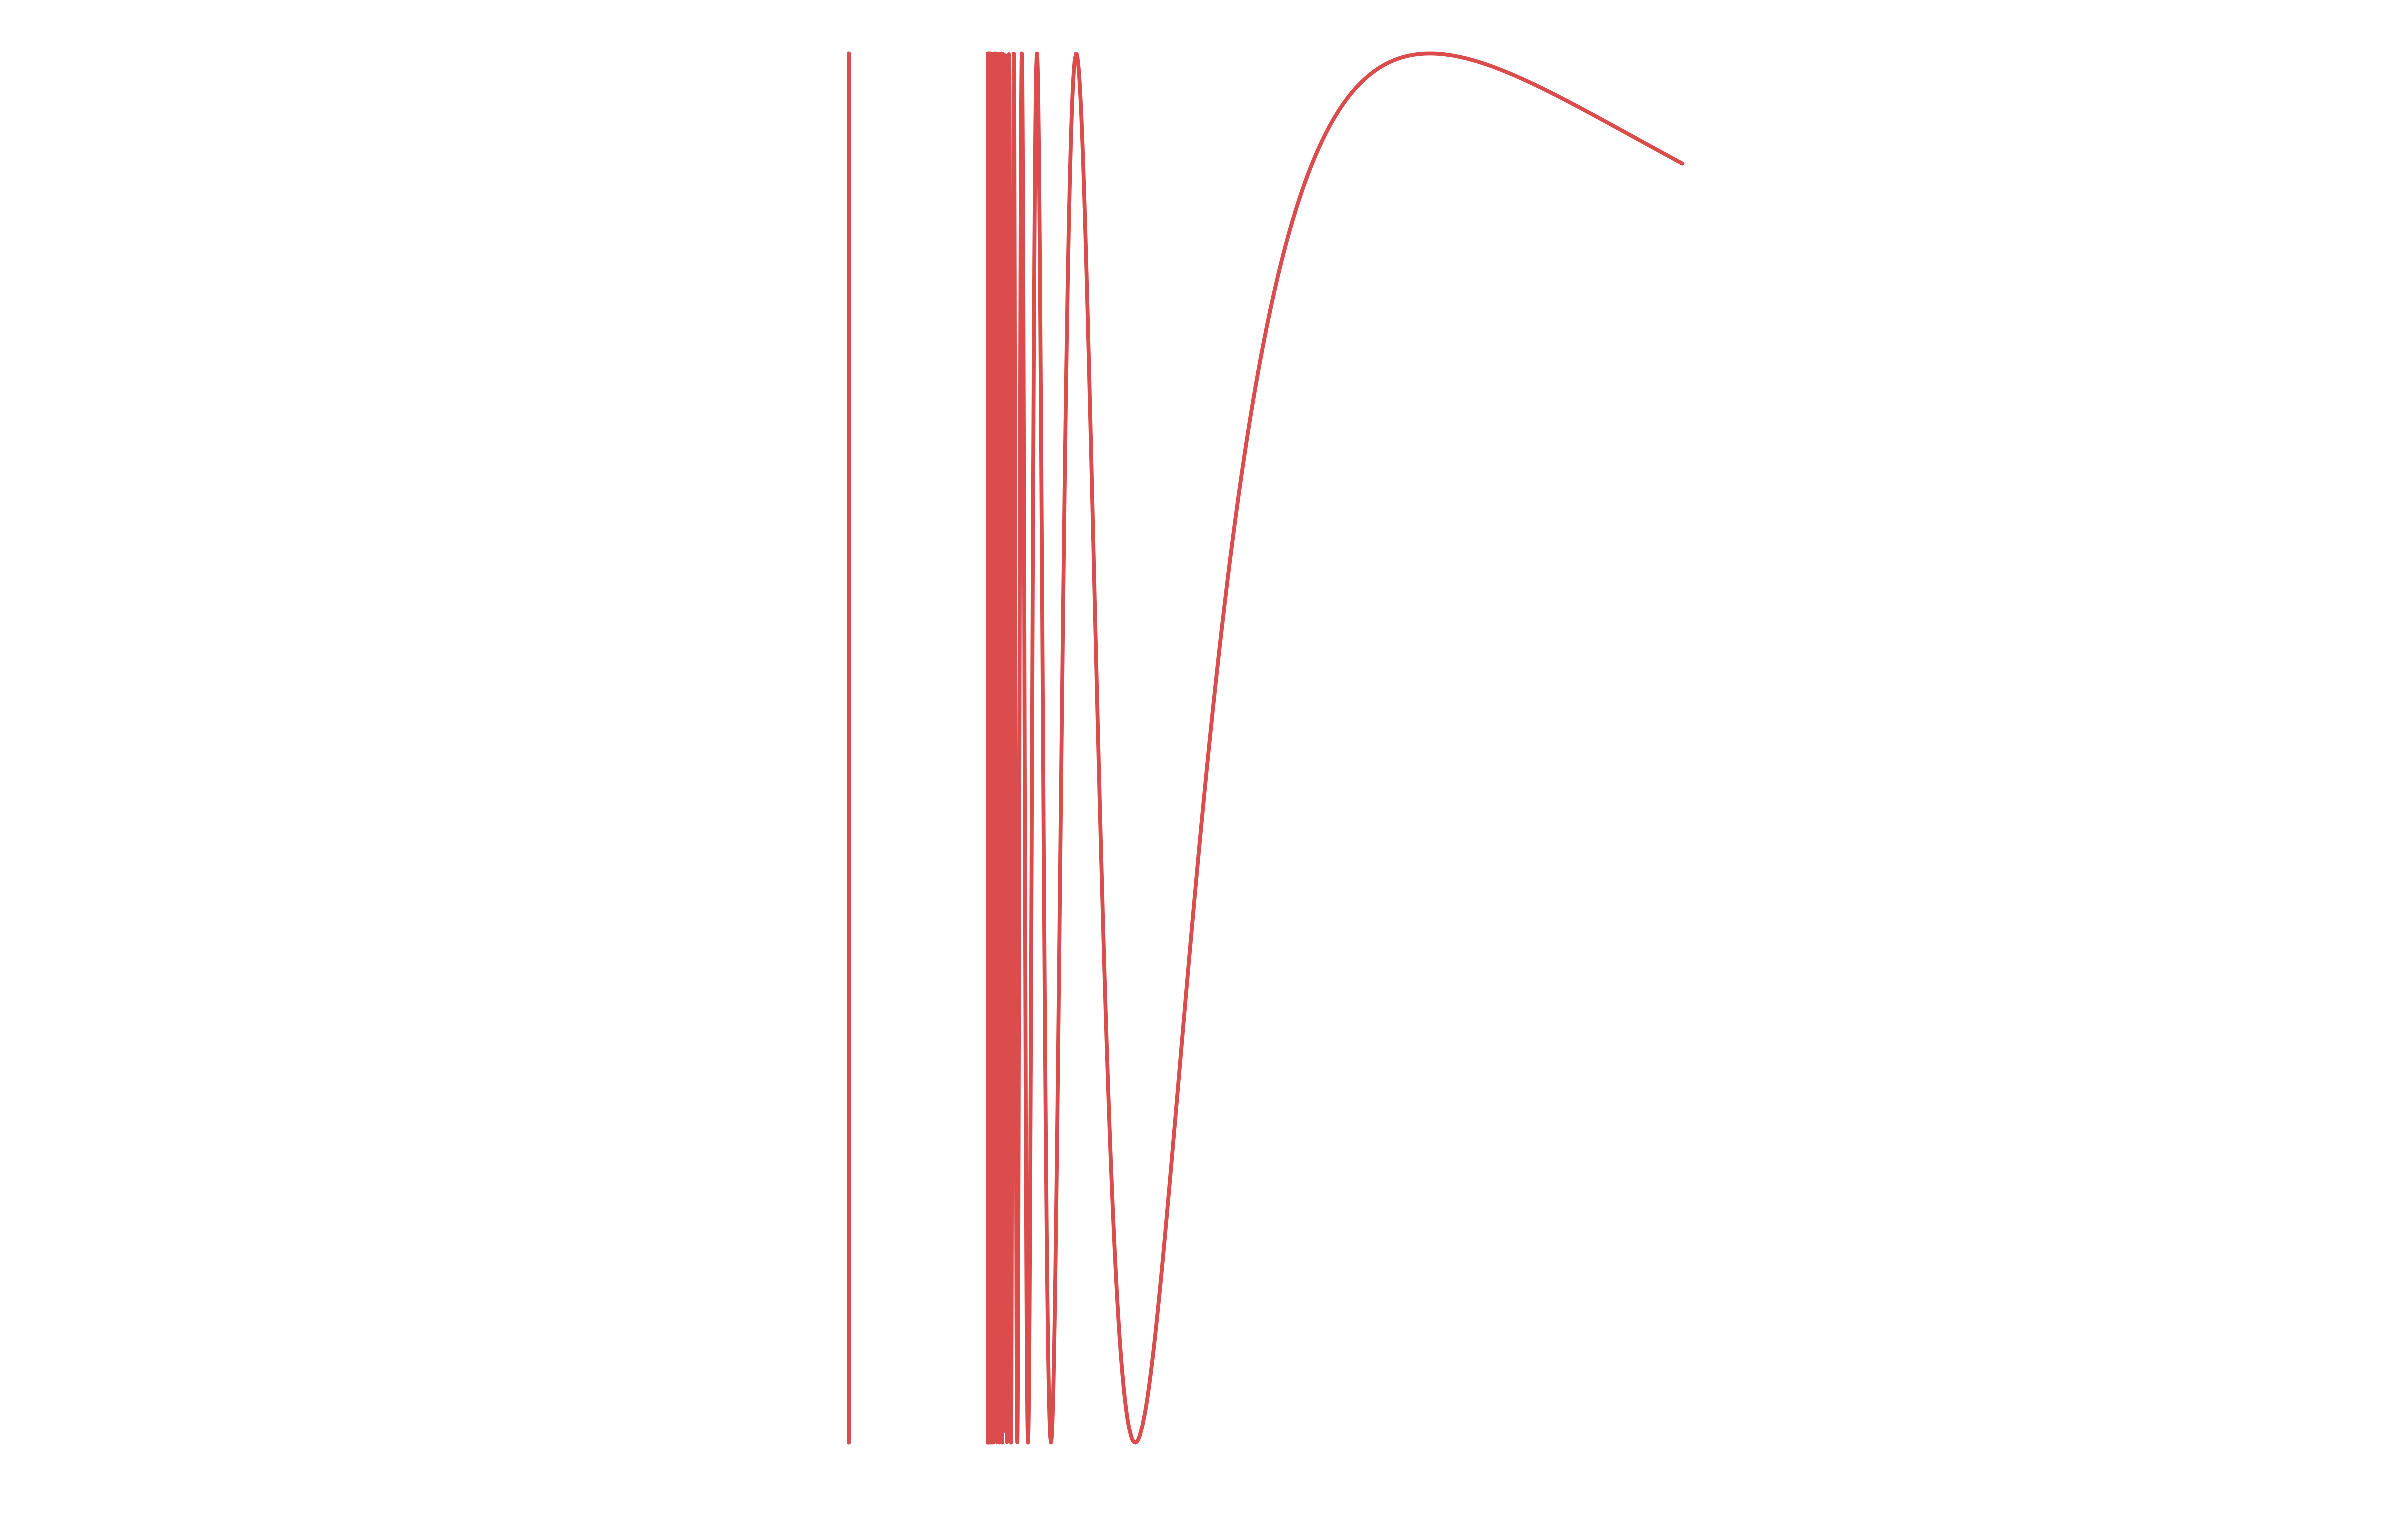
\includegraphics[scale = 0.2]{Figures/Chapter3/topologistsSineCurve.eps}
            \caption{The topologists Sine Curve, defined by $x \times \sin{\frac{1}{x}}$.}
            \label{fig_3.2}
        \end{figure}

        Let $S=\{x \times \sin{\frac{1}{x}}:0 < x \leq 1\}$. This is the image of the continuous map
        $x \rightarrow x \times \sin{\frac{1}{x}$ from $(0,1] \rightarrow \R^2$, Since $(0,1]$ is
            connected, then so is $S$. by theorem \ref{3.1.6}. We call $\cl{S}=S \cup (0 \times
            [-1,1])$ the \textbf{topologist's sine curve} (see figure \ref{fig_3.2}).

            Suppose that $f:[a,c] \rightarrow \cl{S}$ is a path begining at $0$ and ending at a
            point in  $S$. The set  $T=\{t \in \R:f(t) \in 0 \times [-1,1]\}$ is closed, so it has a
            largest element $b$. Then  $f$ is a path mapping  $b \rightarrow 0 \times [-1,1]$ and
            taking all other points to $S$. Suppose that  $[b,c]=[0,1]$ and let $f(t)=(x(t),y(t))$
            where $x(0)=0$, $x(t)>0$ and $y(t)=\sin{\frac{1}{x(t)}}$ for all $t>0$. For  $n \in
            \Z^+$, choose  $0<u<x(\frac{1}{n})$ such that $\sin{\frac{1}{u}}=(-1)^n$. By the
            intermediate value theorem, there are $0<t_n<\frac{1}{n}$ with $x(t_n)=u$. Then the
            sequence $\{t_n\} \rightarrow 0$, and $x(t_n)=(-1)^n$, which diverges; a contradiciton
            since $x(0)=0$ and $\{t_n\} \rightarrow 0$. Hence $\cl{S}$ is not path connected.

    \end{enumerate}
\end{example} 

\section{Outer Measures}

\begin{definition}
    Let $X$ be a set. An \textbf{outer-measure} on $X$ is a function $m^\ast:2^X
    \xrightarrow{} [0, \infty)$ for which the following are true:
    \begin{enumerate}
        \item[(1)] $m^\ast(\emptyset)=0$.

        \item[(2)] If $A \subseteq B$, then $m^\ast(A) \leq m^\ast(B)$.

        \item[(3)] If $\{A_n\}$ is a countable collection of subsets of $X$,
            then
            \begin{equation*}
                m^\ast\Big{(} \bigcup{A_n} \Big{)} \leq \sum{m^\ast(A_n)}
            \end{equation*}
    \end{enumerate}
\end{definition}

\begin{lemma}\label{lemma_1.3.1}
    Let $X$ be a set, and  $\Ec$ a collection of subsets of $X$ for which
    $\emtyset \in \Ec$ and $X \in \Ec$, and let $l:\Ec \xrightarrow{} [0, \infty]$
    a function for which $l(\emptyset)=0$. For any $A \subseteq X$, define
    \begin{equation}\label{equation_1.4}
        m^\ast(A)=\inf{\Big{\{} \sum{l(E_n)} : E_n \in \Ec, \text{ and }
       A \subseteq \bigcup{E_n} \Big{\}}}
    \end{equation}
    Then $m^\ast$ defines an outer-measure.
\end{lemma}
\begin{proof}
    For all $A \subseteq X$, there is a collection $\{E_n\}$ of sets of $\Ec$
    for which $A \subseteq \bigcup{E_n}$. Observe first, that since $l(E_n) \geq
    0$ for all $n$, that  $\sum{l(E_n)} \geq 0$. This makes $m^\ast(A) \geq 0$.
    Now, choose $E_n=\emptyset$ for all  $n$, and we get  $m^\ast(\emptyset)=0$.

    Now, let $A \subseteq B$ subsets of $X$, and let  $\{E_n\}$ a countable
    cover of $B$. Then  $\{E_n\}$ is also a countable cover of $A$. Define then
     $E=\{\sum{l(E_n)} : A \subseteq \bigcup{E_n}\}$ and $F=\{\sum{l(E_n)} :
     B \subseteq \bigcup{E_n}\}$. Since $A \subseteq B$, $F \subseteq E$.
     Therefore, by least upper bounds, we have $\inf{F} \leq \inf{B}$, that is
     $m^\ast(A) \leq m^\ast(B)$.

     Lastly, let $\{A_n\}$ be a countable collection of sets of $X$, and let
     $A=\bigcup{A_n}$. Now, if at least one of the $m(A_n)=\infty$, then we are
     done. Suppose then that $m(A_n)<\infty$ for all $n$. Now, there exists a
     cover of  $A_n$,  $\{E_{n,k}\}_k$ for which
     \begin{equation*}
         \sum_{k}{l(E_{n,k})}<m^\ast(A)+\frac{1}{2^k}
     \end{equation*}
     consider now the countable collection
     $\{E_{n,k}\}_{n,k}=\bigcup_{n}{\{E_{n,k}\}_k}$. Then $\{E_{n,k}\}_{n,k}$ is
     a countable cover for $A$, and we get
     \begin{equation*}
         m^\ast(A) \leq \sum_n{\sum_k{l(E_{n,k})}}<
         \sum_n{m^\ast(A_n)+\frac{1}{2^k}}=\sum_n{m^\ast(A_n)}+\e
     \end{equation*}
     Take then $\e>0$ small, and we get the result.
\end{proof}
\begin{corollary}
    If $E$ is a set of $\Ec$, then $m^\ast(E)=l(E)$.
\end{corollary}
\begin{proof}
    Observe that $E$ covers itself, so that
    $m^\ast(E)=\inf{\{\sum_{i=1}^1{E}\}}=\inf{l(E)}=l(E)$.
\end{proof}

\begin{definition}
    Let $X$ be a set. We call a subset $A$ of  $X$  \textbf{$m^\ast$-measurable}
    if for any subset $E$ of  $X$,
    \begin{equation}\label{equation_1.5}
        m^\ast(E)=m^\ast(E \cap A)+m^\ast(E \cap \com{X}{A})
    \end{equation}
\end{definition}

\begin{lemma}\label{lemma_1.3.2}
    Let $X$ be a set. A subset $A$ of $X$ is  $m^\ast$-measurable if, and only
    if
    \begin{equation*}
        m^\ast(E) \geq m^\ast(E \cap A)+m^\ast(E \cap \com{X}{A}) \text{ for all }
        E \subseteq X
    \end{equation*}
\end{lemma}

\begin{theorem}[Carath\'eodory's Theorem]\label{theorem_1.3.3}
    Let $X$ be a set, and $m^\ast$ an outer-measure on $X$. Then the collection
    of all $m^\ast$-measurable sets forms a  $\s$-algebra. Moreover,  $m^\ast$
    is a complete measure on this $\s$-algebra.
\end{theorem}
\begin{proof}
    Let $\Mc$ be the collection of all  $m^\ast$-measurable sets. Observe first
    that if  $A \in \Mc$, then so is $\com{X}{A}$, by symetry of equation
    \ref{equation_1.5}. So $\Mc$ is closed under complements. Now, let  $A,B \in
    \Mc$. Then we have
    \begin{align*}
        m^\ast(E) &= m^\ast(E \cap A)+m^\ast(E \cap \com{X}{A}) \\
               &= m^\ast(E \cap A \cap B)+m^\ast(E \cap A \cap \com{X}{B})
                        +m^\ast(E \cap B \cap \com{X}{A})+m^\ast(E \cap
                        \com{X}{A} \cap \com{X}{B}) \\
    \end{align*}
    Now, since $A \cup B=(A \cap B) \cup (A \cap \com{X}{B}) \cup (B \cap
    \com{X}{A})$, so by subadditivity, we get
    \begin{equation*}
        m^\ast(E \cap A \cap B)+m^\ast(E \cap A \cap \com{X}{B})+m^\ast(E \cap
        \com{X}{A} \cap B) \geq m^\ast(E \cap (A \cup B))
    \end{equation*}
    i.e. $m^\ast(E) \geq m^\ast(E \cap (A \cup B))+m^\ast(E \cap \com{X}{(A \cup
    B)})$. That is, $A \cup B \in \Mc$, making $\Mc$ an algebra.

    Now, let  $\{A_n\}$ be a countable disjoint collection of
    $m^\ast$-measurable sets, and take  $B_n=\bigcup_{i=1}^n{A_i}$, and take
    $B=\bigcup{B_n}$. Then for all $E \subseteq X$
    \begin{align*}
        m^\ast(E \cap B_n) &= m^\ast(E \cap B_n \cap A_n)+m^\ast(E \cap B_n \cap
                        \com{X}{A_n}) \\
                     &= m^\ast(E \ca A_n)+m^\ast(E \cap B_{n-1})
    \end{align*}
    an induction argument on the collection $\{B_n\}$ gives us
    \begin{equation*}
        m^\ast(E \cap B_n)=\sum_{i=1}^n{m^\ast(E \cap A_i)}
    \end{equation*}
    therefore
    \begin{equation*}
        m^\ast(E)=m^\ast(E \cap B_n)+m^\ast(E \cap \com{X}{B_n}) \geq
        \sum_{i=1}^n{m^\at(E \cap A_i)}+m^\ast(E \cap \com{X}{B_n})
    \end{equation*}
    letting $n \xrightarrow{} \infty$,
    \begin{equation*}
        m^\ast(E) \geq \sum{m^\at(E \cap A_n)}+m^\ast(E \cap \com{X}{B_n})
    \end{equation*}
    so that $B \in \Mc$. Taking $E=B$, we get  $m^\ast(B)=\sum{m^\ast(A_n)}$ so
    that $m^\ast$ is countably additive, and $\Mc$ is a $\s$-algebra.

    Finally, let $m^\ast(A)=0$, then for any $E \subseteq X$, we have
    \begin{equation*}
        m^\ast(E) \leq m^\ast(E \cap A)+m^\ast(E \cap \com{X}{A})=
        m^\ast(E \cap \com{X}{A}) \leq m^\ast(E)
    \end{equation*}
    so that $A \in \Mc$, which makes $m^\ast$ complete on $\Mc$.
\end{proof}

\begin{definition}
    Let $X$ be a set, and  $\Ac$ an algebra on  $X$. We define a
    \textbf{pre-measure} on $\Ac$ to be a function  $m_0:\Ac \xrightarrow{}
    [0,\infty]$ for which
    \begin{enumerate}
        \item[(1)] $m_0(\emptyset)=0$.

        \item[(2)] If $\{A_n\}$ is a countably disjoint collection of sets in
            $\Ac$, for which  $\bigcup{A_n} \in \Ac$, then
            \begin{equation}\label{equation_1.6}
                m_0\Big{(} \bigcup{A_n} \Big{)}=\sum{m_0(A_n)}
            \end{equation}
    \end{enumerate}
\end{definition}

\begin{lemma}\label{lemma_1.3.4}
    Pre-measures on algebras define outer-measures on the overlying sets.
\end{lemma}
\begin{proof}
    Consider the definition of the outer measure $m^\ast$ from equation
    \ref{equation_1.4}, simply take $l=m_0$, and $\Ec=\Ac$.
\end{proof}

\begin{lemma}\label{lemma_1.3.5}
    Let $X$ be a set, and  $\Ac$ an algebra on  $X$. If  $m_0$ is pre-measure on
    $\Ac$, and the measure $m^\ast$ is define by
    \begin{equation*}
        m^\ast(A)=\inf{\Big{\{} \sum{m_0(E_n)} : E_n \in \Ac, \text{ and }
       A \subseteq \bigcup{E_n} \Big{\}}}
    \end{equation*}
    then the following are true.
    \begin{enumerate}
        \item[(1)] $m_0=m^\ast$ on $\Ac$.

        \item[(2)] Every set in $\Ac$ is  $m^\ast$-measurable.
    \end{enumerate}
\end{lemma}
\begin{proof}
    For (1), suppose that $A \in \Ac$, and that $A \subseteq \bigcup{E_n}$ for
    $E_n \in \Ac$. Take
    \begin{equation*}
        F_n=A \cap \com{A_n}{\Big{(} \bigcup_{i=1}^{n-1}{A_i} \Big{)}}
    \end{equation*}
    then $\{F_n\}$ is a disjoint countable collection of sets of $\Ac$ for which
     $A=\bigcup{F_n}$. Hence
     \begin{equation*}
         mo(A)=\sum{m_0(F_n)} \leq \sum{m_0(E_n)}
     \end{equation*}
     it follows from hypothesis that $m_0(A) \leq m^\ast(E)$. For the reverse
     inclusion, simply take $A \subseteq \bigcup{E_n}$ with $A=E_1$ and
     $E_n=\emptyset$ for all  $n>1$.

     For (2), if $A \in \Ac$, and $E \subseteq X$, and $\e>0$, there is a
     collection  $\{B_n\}$ of sets of $\Ac$ with  $A \subseteq \bigcup{B_n}$,
     and
     \begin{equation*}
         \sum{m_0(B_n)}<m^\ast(A)+\e
     \end{equation*}
     by additivity of $m_0$ on $\Ac$, we get
     \begin{equation*}
         m^\ast(E)+\e \geq \sum{m_0(B_n \cap A)}+\sum{m_0(B_n \cap \com{X}{A})}
                    \geq m^\ast(E \cap A)+m^\ast(E \cap \com{X}{A})
     \end{equation*}
\end{proof}

\begin{theorem}\label{theorem_1.3.6}
    Let $X$ be a set, and  $\Ac$ an algerba on  $X$. Let  $m_0$ be a pre-measure
    on $\Ac$, and let  $\Mc$ the  $\s$-algebra generated by  $\Ac$. Then there
    exists a measure  $m$ on  $\Mc$ whose restriction to  $\AC$ is  $m_0$.
    Moreover, if $n$ is another measure extending from $m_0$, then
    \begin{equation*}
        n(E) \leq m(E) \text{ for all } E \in \Mc
    \end{equation*}
    where equality holds when $m(E)<\infty$. Lastly, if $m_0$ is $\s$-finite,
    then  $m$ is the unique extension of  $m_0$ to $\Mc$.
\end{theorem}
\begin{proof}
    Define again,
    \begin{equation*}
        m^\ast(A)=\inf{\Big{\{} \sum{m_0(E_k)} : E_k \in \Ac, \text{ and }
       A \subseteq \bigcup{E_k} \Big{\}}}
    \end{equation*}
    then by Carath\'eodory's theorem, lemma \ref{lemma_1.3.5}, the first result
    follows, since the $\s$-algebra of all  $m^\ast$-measurable sets contains
    $\Ac$, and as consequence, also contains $\Mc$.

    Now, let $E \in \Mc$ with $E \subseteq \bigcup{A_k}$, where $A_k \in \Ac$.
    Then
    \begin{equation*}
        n(E) \leq \sum{n(A_n)}=\sum{m_0(A_n)}
    \end{equation*}
    which gives us $n(E) \leq m(E)$. Now, set $A=\bigcup{A_n}$, and observe that
    \begin{equation*}
        n(A)=\lim_{k \xrightarrow{} \infty}{n\Big{(} \bigcup_{i=1}^k{A_i} \Big{)}}
        =\lim_{k \xrightarrow{} \infty}{m\Big{(} \bigcup_{i=1}^k{A_i}
        \Big{)}}=m(A)
    \end{equation*}
    if $m(E)<\infty$, choose $A_k$ such that  $m(A)<m(E)+\e$ for $\e>0$. Then
    $m(\com{A}{E})<\e$, and
    \begin{equation*}
        m(E) \leq m(A)=n(A)=n(E)+n(\com{A}{E}) \leq n(E)+m(\com{A}{E}) \leq
        n(E)+\e
    \end{equation*}
    taking $\e$ small, we get $n(E)=m(E)$.

    Finally, suppose that $m_0$ is $\s$-finite, and let $X=\bigcup{A_k}$ for
    s me0disjoint collection $\ A_n\}$, then $ m_0 m_0)<\infty$. Then for every
    $E \in \Mc$,
    \begin{equation*}
        m(E)=\sum{m(E \cap A_k)}=\sum{n(E \cap A_k)}=n(E)
    \end{equation*}
    so that $m=n$, making $m$ unique.
\end{proof}

%\section{Roots of Analytic Functions}


%----------------------------------------------------------------------------------------
%	CHAPTER 3
%----------------------------------------------------------------------------------------

\chapter{Continuity on $\R$.} % Main chapter title

\label{Chapter3} % Change X to a consecutive number; for referencing this chapter elsewhere, use \ref{ChapterX}

%% to include section files use the \input{} command.

%----------------------------------------------------------------------------------------
%	SECTION 1.1
%----------------------------------------------------------------------------------------

\section{More on Polynomial Rings.}
\label{section1}

\begin{definition}
    Let $R$ be a commutative ring with identity $1 \neq 0$, and $I$ an ideal of
    $R$. Then
    \begin{equation*}
        \faktor{R[x]}{I[x]} \simeq \faktor{R}{I}[x]
    \end{equation*}
    That is, the factor ring of the polynomial rings is isomorphic to the
    polynomial ring of the factor ring.
\end{definition}

%----------------------------------------------------------------------------------------
%	SECTION 1.1
%----------------------------------------------------------------------------------------

\section{Connected Spaces of The Real Line.}

\begin{definition}
    We call a simply ordered set $L$ with  $|L|>1$ a  \textbf{ordered contunuum} if:
        \begin{enumerate}[label=(\arabic*)]
            \item $L$ has the least upperbound property.

            \item If $x<y$, then there exists a  $z$ such that  $x<z<y$.
        \end{enumerate}
\end{definition}

\begin{theorem}\label{3.2.1}
    If $L$ is a linear continuum in the order topology, then  $L$ is connected, and so are the open
    sets of  $L$  (the intervals and rays in $L$).
\end{theorem}
\begin{proof}
    We show that convex sets are connected. Let $Y=A \cup B$ be a seperation, and choose  $a \in A$,
     $b \in B$ with  $a<b$. We have that the interval of points in  $L$,  $[a,b] \subseteq Y$; and
     we also have that $[a,b] \subseteq A_0 \cup B_0$ with $ A_0=A \cap [a,b]$ and $ B_0=B \cap
     [a,b]$. Now $ A_0,B_0 \neq \emptyset$, so $[a,b]=A_0 \cup B_0$ is a seperation of $[a,b]$. Now
     let $c=\sup{A_0}$. Suppose first that $c \in B_0$, then $c \neq a$, so either $c=b$ or  $a<c<b$.
     Since  $ B_0$ is open in $[a,b]$ as a subspace of $Y$, there is some interval  $(d,c] \subseteq
     B_0$.

     If $c=b$, then  $d<c$ is an upperbound of  $ A_0$, which contradicts that $c$ is the least
     upperbound. Now suppose that $c<b$. We have that since  $c,b \in B_0$, $(c,b] \cap A_0=
     \emptyset$, then $(b,d] \cap A_0=(d,c] \cap (c,b] \cap A_0 = \emptyset$, and again we have
     $d<c$ which gives us the contradiction. So  $c \notin B$. By similar reasoning  $c \notin A_0$.
\end{proof}
\begin{corollary}
    $\R$ is connected and so are the intervals and rays of  $\R$.
\end{corollary}
\begin{proof}
    $\R$ is a linear continuum.
\end{proof}

\begin{theorem}[The Intermediate Value Theorem]\label{3.2.2}
    Let $f:X \rightarrow Y$ be continuous with  $X$ connected, and  $Y$ an ordered set under the
    order topology. If  $a,b \in X$, and if  $r \in Y$ such that  $f(a)<r<f(b)$ or $f(b)<r<f(a)$,
    then there exists a $c \in X$ for which  $f(c)=r$.
\end{theorem}
\begin{proof}
    Let $r \in Y$ such that  $f(a)<r<f(b)$, without loss of generality. We have that $A=f(X) \cap
    (-\infty, r)$ and $B=f(X) \cap (r ,\infty)$ are disjoint, nonempty sets open if $f(X)$ as a
    subspace of $Y$. Now suppose there is no  $c \in X$ for which  $f(c)=r$, then $f(X)=A \cup B$ is
    a seperation of $f(X)$, which contradicts theorem \ref{3.1.6}.
\end{proof}

\begin{example}
    \begin{enumerate}[label=(\arabic*)]
        \item The ordered square $I_0^2$ is a linera continuum. Let $A \subseteq I_0^2$ and consider
            the projection $\pi_1:I_0^2 \rightarrow I_0^2$. Let $b=\sup{\pi_1(A)}$, now if $b \in
            \pi_1(A)$ then $A \cap (b \times I_0) \neq \emptyset$, and since $I_0 \subseteq \R$, $A
            \cap (b \times I_0)$ has a least upperbound, $b \times c$, where  $c=\sup{I_0}$, which
            is also the least upperbound of $A$. Now if we have $a \times c < b \times d$, then
            $a<b$ and  $c<d$; and since  $\R$ is a linear continuum, there are $y,z \in \R$ for
            which  $a<y<b$ and  $c<z<d$. Hence  $a \times c < y \times z < b \times d$; which makes
            $ I_0^2$ into a liear continuum.

        \item If $X$ is a well ordered set, then  $X \times [0,1)$ is a linear contiuum in the
            dictionary order. Let $A \subseteq X \times [0,1)$ and consider the projection $\pi_2:X
            \times [0,1) \rightarrow [0,1)$. If $b=\sup{\pi_2(A)}$, then $A \cap (b \times [0,1)) \neq
            0$, and so $A \cap (b \times [0,1)$ has a least upperbound $b \times c$ with
            $c=\sup{[0,1)}$, which is also a least upperbound of $A$.

            Now since $\R$ is a linear continuum, if $x \times a < y \times b$, under the dictionary
            order, then  $x \leq y$ and  $a<b$. Then there are  $c,z \in \R$ such that  $x \leq z
            \leq y$ and  $a<c<b$, so that $x \times a < z \times c < y \times b$.
    \end{enumerate}
\end{example} 

\begin{definition}
    Let $X$ be a topological space with  $x, y \in X$. A \textbf{$xy$-path} in $X$ from  $x$ to  $y$ is a
    continuous map  $f:[a,b] \rightarrow X$, with $[a,b] \subseteq \R$ such that $f(a)=x$, and
    $f(b)=y$. We call $X$ \textbf {path connected} if there exists an $xy$-path in $X$ for every
    $x,y \in X$.
\end{definition}

\begin{theorem}\label{3.2.3}
    Path connected spaces are connected
\end{theorem}
\begin{proof}
    Let $X$ be path connected, and suppose that  $X=A \cup B$ is a seperation of  $X$. Let  $f:[a,b]
    \rightarrow X$ be some path in $X$. Since  $f$ is continuous, and  $[a,b] \subseteq \R$, by
    theorem \ref{3.1.6}, $f([a,b]) \subseteq X$ is a connected subspace, so either $f([a,b])
    \subseteq A$ or $f([a,b]) \subseteq B$, so there is no path from a point in $A$ to a point in
    $B$. But  $X$ is path connected; a contradiction. Therefore  $X$ must be connected.
\end{proof}

\begin{example}
    \begin{enumerate}[label=(\arabic*)]
        \item Define the \textbf{unit ball} in $\R^n$ under  $||\cdot||$ to be  $B^n=\{x \in
            \R^n:||x|| \leq 1\}$. $B^n$ is path connected. Consider  $f[0,1] \rightarrow B^n$ by
            $f(t)=(1-t)x+ty$, then $||f(t)||=(1-t)||x||+t||y|| \leq 1$, hence $f(t) \in  B^n$.
            Extending this to arbitrariy balls, for $\epsilon>0$, $B(x,\epsilon)$ and
            $cl{B(x,\epsilon)}$ are also path connected. The function $f$ also shows that the unit
            ball, and open balls  (as well as their closure) are convex.

        \item Define \textbf{punctured Euclidean space} to be $\com{\R^n}{\{0\}}$. If $n>1$,
        $\com{\R}{\{0\}}$ is path connected. Connect the points $x,y \in \com{\R^n}{\{0\}}$ by a
        straight line not passing through $0$, or choose a point $z \in \com{\R^n}{\{0\}}$ on that
        line and form a path by adjoining the lines from $x$ to  $z$ and from  $z$ to  $y$

        \begin{figure}[h] 
            \centering
            
\includegraphics[scale=0.2]{Figures/Chapter3/puncturedSpace.eps}
            \caption{Punctures $2$-space $\com{\R^2}{\{0\}}$.}
            \label{fig_3.1}
        \end{figure}

    \item Consider the unit sphere $S^{n-1}=\{x \in \R^n:||x||=1\}$ in $\R^n$.  $S^{n_-1}$ is path
        connected for $n>1$. Take the map  $g:\com{\R^n}\{0\} \rightarrow S^{n-1}$ by $g:x
        \rightarrow \frac{x}{||x||}$.

    \item The ordered square $ I_0^2$ is connected, but it is not path connected/ Let $p=0 \times
        0$,  $1=1 \times 1$ and let  $f:[a,b] \rightarrow I_0^2$ be a path joining $p$ and  $q$. We
        have that  $f([a,b])$ must contain all $x \times y \in I_0^2$ by the intermediate value
        theorem. Hence for each  $x \in I_0$, $U_x=f^{-1}(x \times I_0) \neq \emptyset$ and it is
        also open in $[a,b]$. Now choose for each $x \in I_0$, $q_x \in \Q$ such that  $q_x \in
        U_x$. Since  $\bigcap_{x \in I_0}{U_x} = \emptyset$, the map $x \rightarrow q_x$ is  $1-1$
        of  $I_0$ onto $\Q$. which makes $I_0$ countable; a contradiction.

    \item 
        \begin{figure}[h]
            \centering
            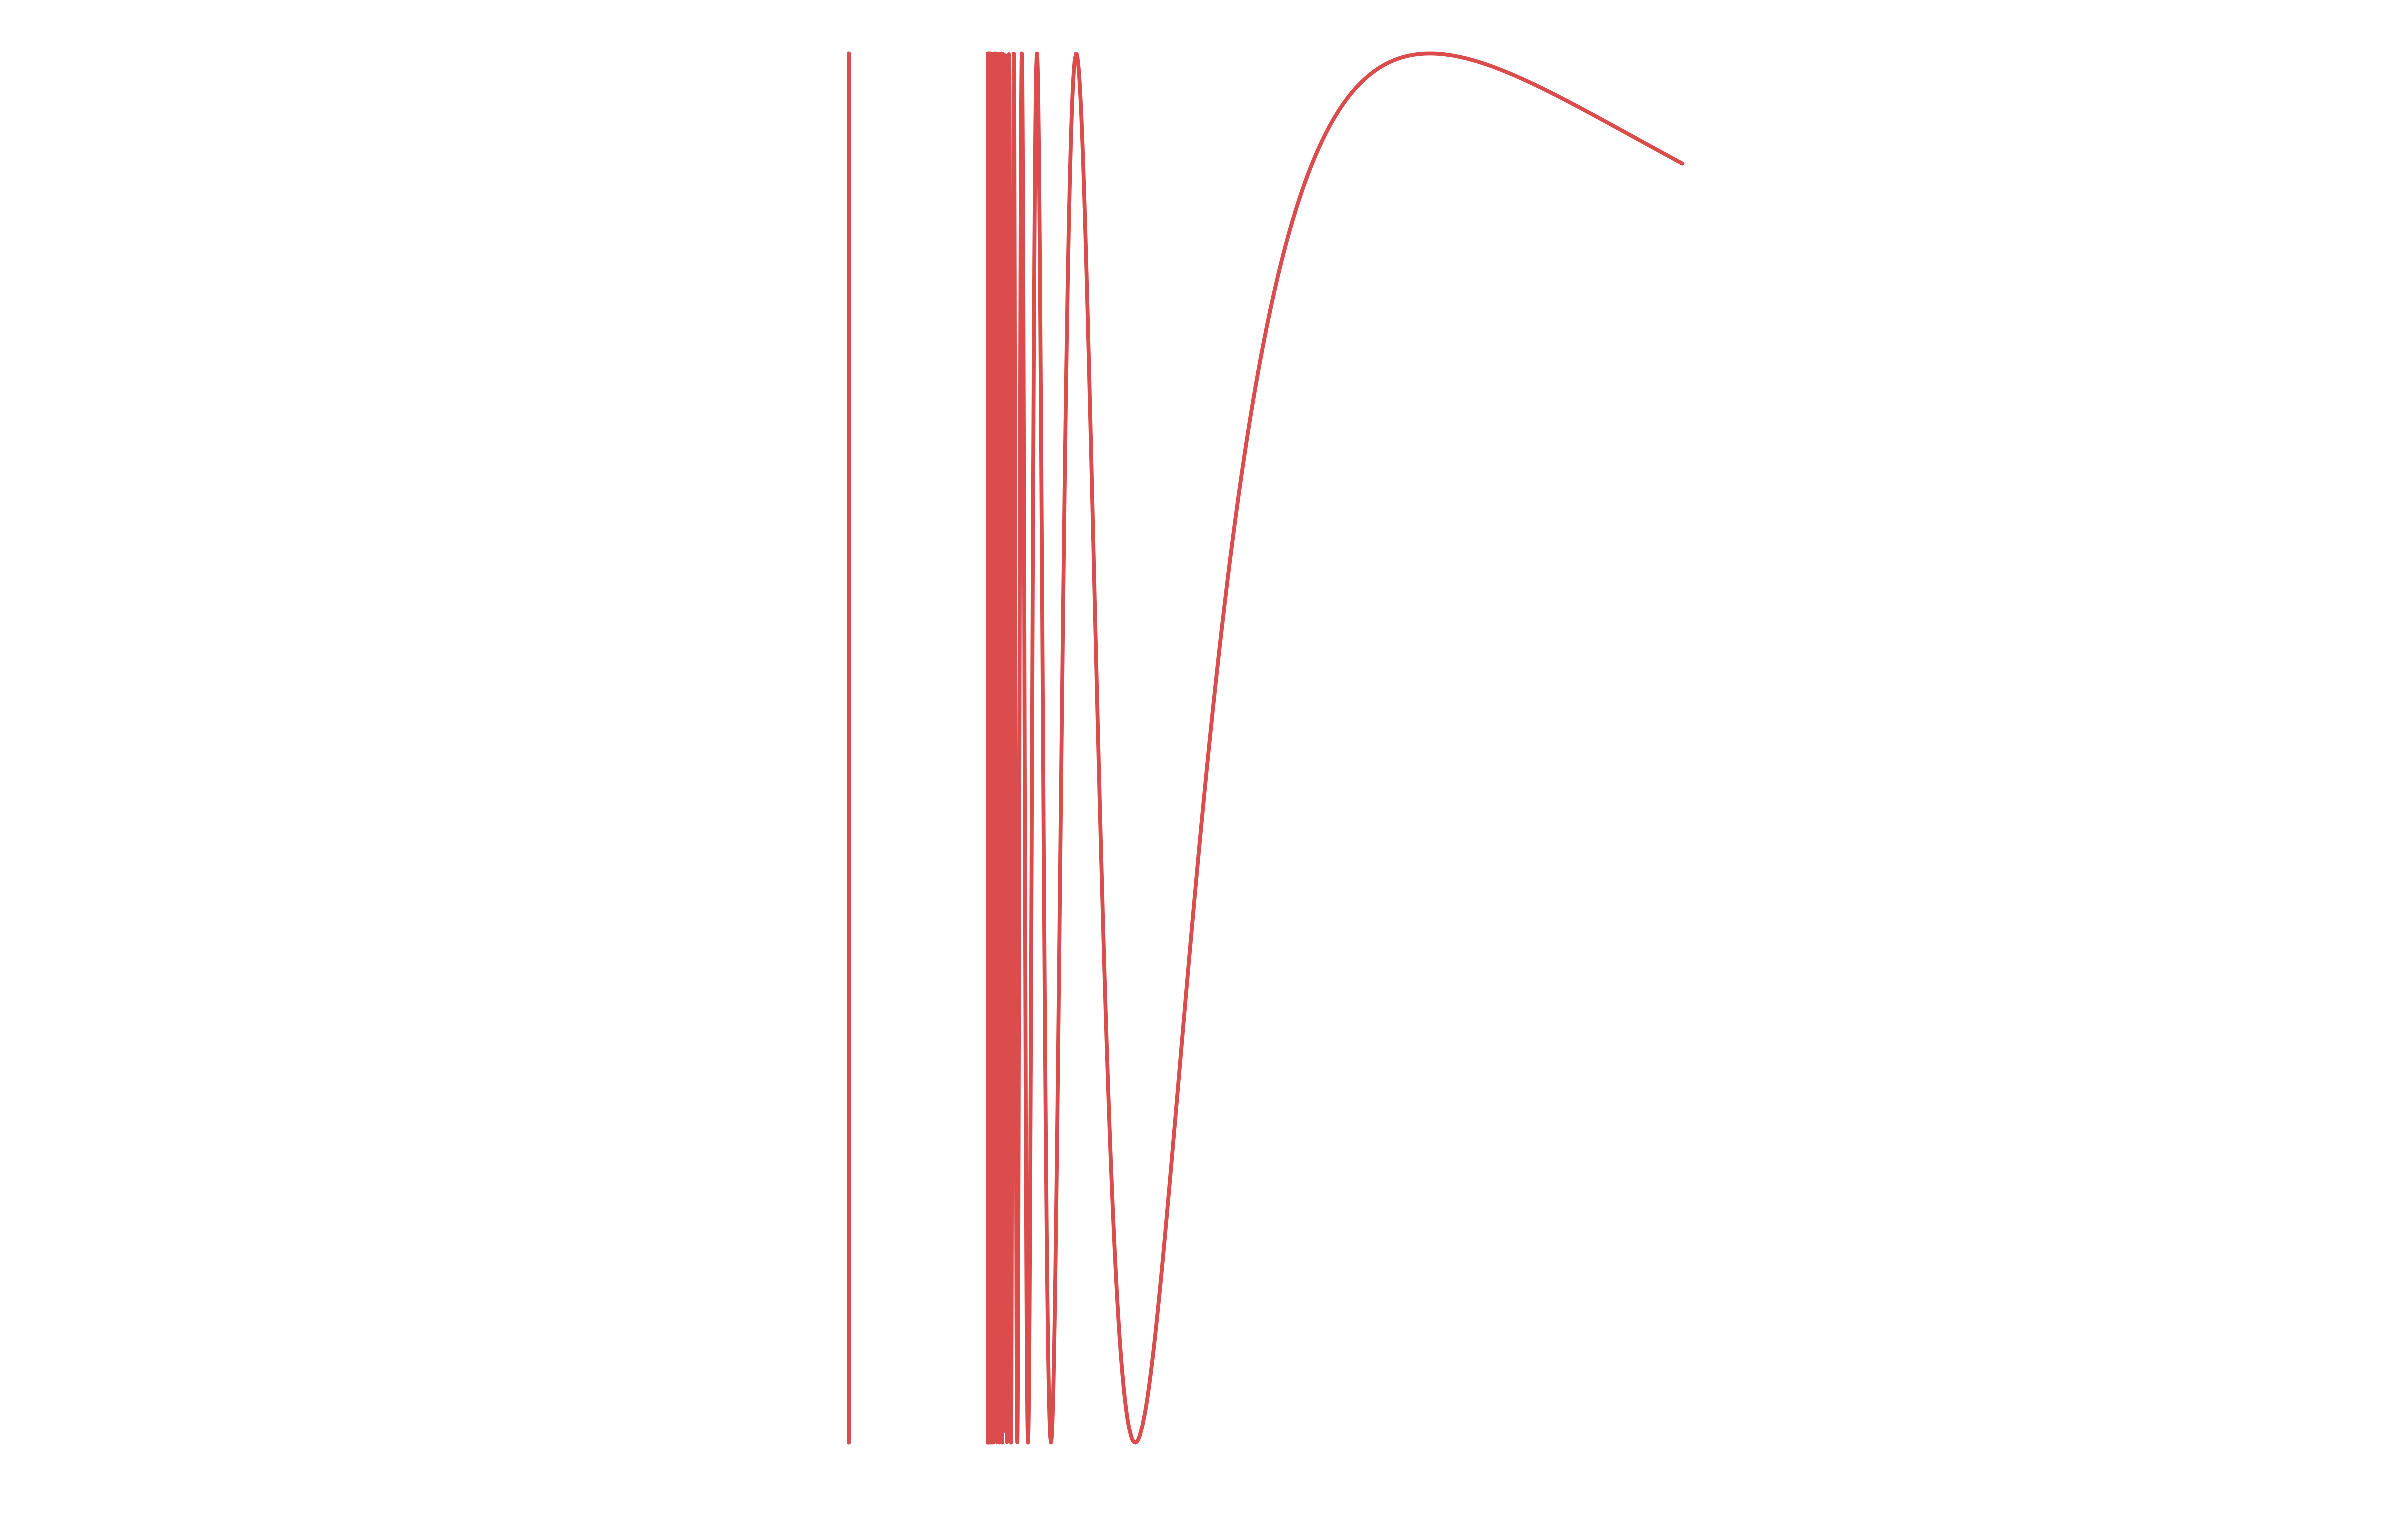
\includegraphics[scale = 0.2]{Figures/Chapter3/topologistsSineCurve.eps}
            \caption{The topologists Sine Curve, defined by $x \times \sin{\frac{1}{x}}$.}
            \label{fig_3.2}
        \end{figure}

        Let $S=\{x \times \sin{\frac{1}{x}}:0 < x \leq 1\}$. This is the image of the continuous map
        $x \rightarrow x \times \sin{\frac{1}{x}$ from $(0,1] \rightarrow \R^2$, Since $(0,1]$ is
            connected, then so is $S$. by theorem \ref{3.1.6}. We call $\cl{S}=S \cup (0 \times
            [-1,1])$ the \textbf{topologist's sine curve} (see figure \ref{fig_3.2}).

            Suppose that $f:[a,c] \rightarrow \cl{S}$ is a path begining at $0$ and ending at a
            point in  $S$. The set  $T=\{t \in \R:f(t) \in 0 \times [-1,1]\}$ is closed, so it has a
            largest element $b$. Then  $f$ is a path mapping  $b \rightarrow 0 \times [-1,1]$ and
            taking all other points to $S$. Suppose that  $[b,c]=[0,1]$ and let $f(t)=(x(t),y(t))$
            where $x(0)=0$, $x(t)>0$ and $y(t)=\sin{\frac{1}{x(t)}}$ for all $t>0$. For  $n \in
            \Z^+$, choose  $0<u<x(\frac{1}{n})$ such that $\sin{\frac{1}{u}}=(-1)^n$. By the
            intermediate value theorem, there are $0<t_n<\frac{1}{n}$ with $x(t_n)=u$. Then the
            sequence $\{t_n\} \rightarrow 0$, and $x(t_n)=(-1)^n$, which diverges; a contradiciton
            since $x(0)=0$ and $\{t_n\} \rightarrow 0$. Hence $\cl{S}$ is not path connected.

    \end{enumerate}
\end{example} 

\section{Outer Measures}

\begin{definition}
    Let $X$ be a set. An \textbf{outer-measure} on $X$ is a function $m^\ast:2^X
    \xrightarrow{} [0, \infty)$ for which the following are true:
    \begin{enumerate}
        \item[(1)] $m^\ast(\emptyset)=0$.

        \item[(2)] If $A \subseteq B$, then $m^\ast(A) \leq m^\ast(B)$.

        \item[(3)] If $\{A_n\}$ is a countable collection of subsets of $X$,
            then
            \begin{equation*}
                m^\ast\Big{(} \bigcup{A_n} \Big{)} \leq \sum{m^\ast(A_n)}
            \end{equation*}
    \end{enumerate}
\end{definition}

\begin{lemma}\label{lemma_1.3.1}
    Let $X$ be a set, and  $\Ec$ a collection of subsets of $X$ for which
    $\emtyset \in \Ec$ and $X \in \Ec$, and let $l:\Ec \xrightarrow{} [0, \infty]$
    a function for which $l(\emptyset)=0$. For any $A \subseteq X$, define
    \begin{equation}\label{equation_1.4}
        m^\ast(A)=\inf{\Big{\{} \sum{l(E_n)} : E_n \in \Ec, \text{ and }
       A \subseteq \bigcup{E_n} \Big{\}}}
    \end{equation}
    Then $m^\ast$ defines an outer-measure.
\end{lemma}
\begin{proof}
    For all $A \subseteq X$, there is a collection $\{E_n\}$ of sets of $\Ec$
    for which $A \subseteq \bigcup{E_n}$. Observe first, that since $l(E_n) \geq
    0$ for all $n$, that  $\sum{l(E_n)} \geq 0$. This makes $m^\ast(A) \geq 0$.
    Now, choose $E_n=\emptyset$ for all  $n$, and we get  $m^\ast(\emptyset)=0$.

    Now, let $A \subseteq B$ subsets of $X$, and let  $\{E_n\}$ a countable
    cover of $B$. Then  $\{E_n\}$ is also a countable cover of $A$. Define then
     $E=\{\sum{l(E_n)} : A \subseteq \bigcup{E_n}\}$ and $F=\{\sum{l(E_n)} :
     B \subseteq \bigcup{E_n}\}$. Since $A \subseteq B$, $F \subseteq E$.
     Therefore, by least upper bounds, we have $\inf{F} \leq \inf{B}$, that is
     $m^\ast(A) \leq m^\ast(B)$.

     Lastly, let $\{A_n\}$ be a countable collection of sets of $X$, and let
     $A=\bigcup{A_n}$. Now, if at least one of the $m(A_n)=\infty$, then we are
     done. Suppose then that $m(A_n)<\infty$ for all $n$. Now, there exists a
     cover of  $A_n$,  $\{E_{n,k}\}_k$ for which
     \begin{equation*}
         \sum_{k}{l(E_{n,k})}<m^\ast(A)+\frac{1}{2^k}
     \end{equation*}
     consider now the countable collection
     $\{E_{n,k}\}_{n,k}=\bigcup_{n}{\{E_{n,k}\}_k}$. Then $\{E_{n,k}\}_{n,k}$ is
     a countable cover for $A$, and we get
     \begin{equation*}
         m^\ast(A) \leq \sum_n{\sum_k{l(E_{n,k})}}<
         \sum_n{m^\ast(A_n)+\frac{1}{2^k}}=\sum_n{m^\ast(A_n)}+\e
     \end{equation*}
     Take then $\e>0$ small, and we get the result.
\end{proof}
\begin{corollary}
    If $E$ is a set of $\Ec$, then $m^\ast(E)=l(E)$.
\end{corollary}
\begin{proof}
    Observe that $E$ covers itself, so that
    $m^\ast(E)=\inf{\{\sum_{i=1}^1{E}\}}=\inf{l(E)}=l(E)$.
\end{proof}

\begin{definition}
    Let $X$ be a set. We call a subset $A$ of  $X$  \textbf{$m^\ast$-measurable}
    if for any subset $E$ of  $X$,
    \begin{equation}\label{equation_1.5}
        m^\ast(E)=m^\ast(E \cap A)+m^\ast(E \cap \com{X}{A})
    \end{equation}
\end{definition}

\begin{lemma}\label{lemma_1.3.2}
    Let $X$ be a set. A subset $A$ of $X$ is  $m^\ast$-measurable if, and only
    if
    \begin{equation*}
        m^\ast(E) \geq m^\ast(E \cap A)+m^\ast(E \cap \com{X}{A}) \text{ for all }
        E \subseteq X
    \end{equation*}
\end{lemma}

\begin{theorem}[Carath\'eodory's Theorem]\label{theorem_1.3.3}
    Let $X$ be a set, and $m^\ast$ an outer-measure on $X$. Then the collection
    of all $m^\ast$-measurable sets forms a  $\s$-algebra. Moreover,  $m^\ast$
    is a complete measure on this $\s$-algebra.
\end{theorem}
\begin{proof}
    Let $\Mc$ be the collection of all  $m^\ast$-measurable sets. Observe first
    that if  $A \in \Mc$, then so is $\com{X}{A}$, by symetry of equation
    \ref{equation_1.5}. So $\Mc$ is closed under complements. Now, let  $A,B \in
    \Mc$. Then we have
    \begin{align*}
        m^\ast(E) &= m^\ast(E \cap A)+m^\ast(E \cap \com{X}{A}) \\
               &= m^\ast(E \cap A \cap B)+m^\ast(E \cap A \cap \com{X}{B})
                        +m^\ast(E \cap B \cap \com{X}{A})+m^\ast(E \cap
                        \com{X}{A} \cap \com{X}{B}) \\
    \end{align*}
    Now, since $A \cup B=(A \cap B) \cup (A \cap \com{X}{B}) \cup (B \cap
    \com{X}{A})$, so by subadditivity, we get
    \begin{equation*}
        m^\ast(E \cap A \cap B)+m^\ast(E \cap A \cap \com{X}{B})+m^\ast(E \cap
        \com{X}{A} \cap B) \geq m^\ast(E \cap (A \cup B))
    \end{equation*}
    i.e. $m^\ast(E) \geq m^\ast(E \cap (A \cup B))+m^\ast(E \cap \com{X}{(A \cup
    B)})$. That is, $A \cup B \in \Mc$, making $\Mc$ an algebra.

    Now, let  $\{A_n\}$ be a countable disjoint collection of
    $m^\ast$-measurable sets, and take  $B_n=\bigcup_{i=1}^n{A_i}$, and take
    $B=\bigcup{B_n}$. Then for all $E \subseteq X$
    \begin{align*}
        m^\ast(E \cap B_n) &= m^\ast(E \cap B_n \cap A_n)+m^\ast(E \cap B_n \cap
                        \com{X}{A_n}) \\
                     &= m^\ast(E \ca A_n)+m^\ast(E \cap B_{n-1})
    \end{align*}
    an induction argument on the collection $\{B_n\}$ gives us
    \begin{equation*}
        m^\ast(E \cap B_n)=\sum_{i=1}^n{m^\ast(E \cap A_i)}
    \end{equation*}
    therefore
    \begin{equation*}
        m^\ast(E)=m^\ast(E \cap B_n)+m^\ast(E \cap \com{X}{B_n}) \geq
        \sum_{i=1}^n{m^\at(E \cap A_i)}+m^\ast(E \cap \com{X}{B_n})
    \end{equation*}
    letting $n \xrightarrow{} \infty$,
    \begin{equation*}
        m^\ast(E) \geq \sum{m^\at(E \cap A_n)}+m^\ast(E \cap \com{X}{B_n})
    \end{equation*}
    so that $B \in \Mc$. Taking $E=B$, we get  $m^\ast(B)=\sum{m^\ast(A_n)}$ so
    that $m^\ast$ is countably additive, and $\Mc$ is a $\s$-algebra.

    Finally, let $m^\ast(A)=0$, then for any $E \subseteq X$, we have
    \begin{equation*}
        m^\ast(E) \leq m^\ast(E \cap A)+m^\ast(E \cap \com{X}{A})=
        m^\ast(E \cap \com{X}{A}) \leq m^\ast(E)
    \end{equation*}
    so that $A \in \Mc$, which makes $m^\ast$ complete on $\Mc$.
\end{proof}

\begin{definition}
    Let $X$ be a set, and  $\Ac$ an algebra on  $X$. We define a
    \textbf{pre-measure} on $\Ac$ to be a function  $m_0:\Ac \xrightarrow{}
    [0,\infty]$ for which
    \begin{enumerate}
        \item[(1)] $m_0(\emptyset)=0$.

        \item[(2)] If $\{A_n\}$ is a countably disjoint collection of sets in
            $\Ac$, for which  $\bigcup{A_n} \in \Ac$, then
            \begin{equation}\label{equation_1.6}
                m_0\Big{(} \bigcup{A_n} \Big{)}=\sum{m_0(A_n)}
            \end{equation}
    \end{enumerate}
\end{definition}

\begin{lemma}\label{lemma_1.3.4}
    Pre-measures on algebras define outer-measures on the overlying sets.
\end{lemma}
\begin{proof}
    Consider the definition of the outer measure $m^\ast$ from equation
    \ref{equation_1.4}, simply take $l=m_0$, and $\Ec=\Ac$.
\end{proof}

\begin{lemma}\label{lemma_1.3.5}
    Let $X$ be a set, and  $\Ac$ an algebra on  $X$. If  $m_0$ is pre-measure on
    $\Ac$, and the measure $m^\ast$ is define by
    \begin{equation*}
        m^\ast(A)=\inf{\Big{\{} \sum{m_0(E_n)} : E_n \in \Ac, \text{ and }
       A \subseteq \bigcup{E_n} \Big{\}}}
    \end{equation*}
    then the following are true.
    \begin{enumerate}
        \item[(1)] $m_0=m^\ast$ on $\Ac$.

        \item[(2)] Every set in $\Ac$ is  $m^\ast$-measurable.
    \end{enumerate}
\end{lemma}
\begin{proof}
    For (1), suppose that $A \in \Ac$, and that $A \subseteq \bigcup{E_n}$ for
    $E_n \in \Ac$. Take
    \begin{equation*}
        F_n=A \cap \com{A_n}{\Big{(} \bigcup_{i=1}^{n-1}{A_i} \Big{)}}
    \end{equation*}
    then $\{F_n\}$ is a disjoint countable collection of sets of $\Ac$ for which
     $A=\bigcup{F_n}$. Hence
     \begin{equation*}
         mo(A)=\sum{m_0(F_n)} \leq \sum{m_0(E_n)}
     \end{equation*}
     it follows from hypothesis that $m_0(A) \leq m^\ast(E)$. For the reverse
     inclusion, simply take $A \subseteq \bigcup{E_n}$ with $A=E_1$ and
     $E_n=\emptyset$ for all  $n>1$.

     For (2), if $A \in \Ac$, and $E \subseteq X$, and $\e>0$, there is a
     collection  $\{B_n\}$ of sets of $\Ac$ with  $A \subseteq \bigcup{B_n}$,
     and
     \begin{equation*}
         \sum{m_0(B_n)}<m^\ast(A)+\e
     \end{equation*}
     by additivity of $m_0$ on $\Ac$, we get
     \begin{equation*}
         m^\ast(E)+\e \geq \sum{m_0(B_n \cap A)}+\sum{m_0(B_n \cap \com{X}{A})}
                    \geq m^\ast(E \cap A)+m^\ast(E \cap \com{X}{A})
     \end{equation*}
\end{proof}

\begin{theorem}\label{theorem_1.3.6}
    Let $X$ be a set, and  $\Ac$ an algerba on  $X$. Let  $m_0$ be a pre-measure
    on $\Ac$, and let  $\Mc$ the  $\s$-algebra generated by  $\Ac$. Then there
    exists a measure  $m$ on  $\Mc$ whose restriction to  $\AC$ is  $m_0$.
    Moreover, if $n$ is another measure extending from $m_0$, then
    \begin{equation*}
        n(E) \leq m(E) \text{ for all } E \in \Mc
    \end{equation*}
    where equality holds when $m(E)<\infty$. Lastly, if $m_0$ is $\s$-finite,
    then  $m$ is the unique extension of  $m_0$ to $\Mc$.
\end{theorem}
\begin{proof}
    Define again,
    \begin{equation*}
        m^\ast(A)=\inf{\Big{\{} \sum{m_0(E_k)} : E_k \in \Ac, \text{ and }
       A \subseteq \bigcup{E_k} \Big{\}}}
    \end{equation*}
    then by Carath\'eodory's theorem, lemma \ref{lemma_1.3.5}, the first result
    follows, since the $\s$-algebra of all  $m^\ast$-measurable sets contains
    $\Ac$, and as consequence, also contains $\Mc$.

    Now, let $E \in \Mc$ with $E \subseteq \bigcup{A_k}$, where $A_k \in \Ac$.
    Then
    \begin{equation*}
        n(E) \leq \sum{n(A_n)}=\sum{m_0(A_n)}
    \end{equation*}
    which gives us $n(E) \leq m(E)$. Now, set $A=\bigcup{A_n}$, and observe that
    \begin{equation*}
        n(A)=\lim_{k \xrightarrow{} \infty}{n\Big{(} \bigcup_{i=1}^k{A_i} \Big{)}}
        =\lim_{k \xrightarrow{} \infty}{m\Big{(} \bigcup_{i=1}^k{A_i}
        \Big{)}}=m(A)
    \end{equation*}
    if $m(E)<\infty$, choose $A_k$ such that  $m(A)<m(E)+\e$ for $\e>0$. Then
    $m(\com{A}{E})<\e$, and
    \begin{equation*}
        m(E) \leq m(A)=n(A)=n(E)+n(\com{A}{E}) \leq n(E)+m(\com{A}{E}) \leq
        n(E)+\e
    \end{equation*}
    taking $\e$ small, we get $n(E)=m(E)$.

    Finally, suppose that $m_0$ is $\s$-finite, and let $X=\bigcup{A_k}$ for
    s me0disjoint collection $\ A_n\}$, then $ m_0 m_0)<\infty$. Then for every
    $E \in \Mc$,
    \begin{equation*}
        m(E)=\sum{m(E \cap A_k)}=\sum{n(E \cap A_k)}=n(E)
    \end{equation*}
    so that $m=n$, making $m$ unique.
\end{proof}

\section{Roots of Analytic Functions}


\chapter{Complex Integration} % Main chapter title

\label{chapter4} %4Change X to a consecutive number; for referencing this chapter elsewhere, use \ref{chapterX}

%% to include section files use the \input{} command.

%----------------------------------------------------------------------------------------
%	SECTION 1.1
%----------------------------------------------------------------------------------------

\section{More on Polynomial Rings.}
\label{section1}

\begin{definition}
    Let $R$ be a commutative ring with identity $1 \neq 0$, and $I$ an ideal of
    $R$. Then
    \begin{equation*}
        \faktor{R[x]}{I[x]} \simeq \faktor{R}{I}[x]
    \end{equation*}
    That is, the factor ring of the polynomial rings is isomorphic to the
    polynomial ring of the factor ring.
\end{definition}

%----------------------------------------------------------------------------------------
%	SECTION 1.1
%----------------------------------------------------------------------------------------

\section{Connected Spaces of The Real Line.}

\begin{definition}
    We call a simply ordered set $L$ with  $|L|>1$ a  \textbf{ordered contunuum} if:
        \begin{enumerate}[label=(\arabic*)]
            \item $L$ has the least upperbound property.

            \item If $x<y$, then there exists a  $z$ such that  $x<z<y$.
        \end{enumerate}
\end{definition}

\begin{theorem}\label{3.2.1}
    If $L$ is a linear continuum in the order topology, then  $L$ is connected, and so are the open
    sets of  $L$  (the intervals and rays in $L$).
\end{theorem}
\begin{proof}
    We show that convex sets are connected. Let $Y=A \cup B$ be a seperation, and choose  $a \in A$,
     $b \in B$ with  $a<b$. We have that the interval of points in  $L$,  $[a,b] \subseteq Y$; and
     we also have that $[a,b] \subseteq A_0 \cup B_0$ with $ A_0=A \cap [a,b]$ and $ B_0=B \cap
     [a,b]$. Now $ A_0,B_0 \neq \emptyset$, so $[a,b]=A_0 \cup B_0$ is a seperation of $[a,b]$. Now
     let $c=\sup{A_0}$. Suppose first that $c \in B_0$, then $c \neq a$, so either $c=b$ or  $a<c<b$.
     Since  $ B_0$ is open in $[a,b]$ as a subspace of $Y$, there is some interval  $(d,c] \subseteq
     B_0$.

     If $c=b$, then  $d<c$ is an upperbound of  $ A_0$, which contradicts that $c$ is the least
     upperbound. Now suppose that $c<b$. We have that since  $c,b \in B_0$, $(c,b] \cap A_0=
     \emptyset$, then $(b,d] \cap A_0=(d,c] \cap (c,b] \cap A_0 = \emptyset$, and again we have
     $d<c$ which gives us the contradiction. So  $c \notin B$. By similar reasoning  $c \notin A_0$.
\end{proof}
\begin{corollary}
    $\R$ is connected and so are the intervals and rays of  $\R$.
\end{corollary}
\begin{proof}
    $\R$ is a linear continuum.
\end{proof}

\begin{theorem}[The Intermediate Value Theorem]\label{3.2.2}
    Let $f:X \rightarrow Y$ be continuous with  $X$ connected, and  $Y$ an ordered set under the
    order topology. If  $a,b \in X$, and if  $r \in Y$ such that  $f(a)<r<f(b)$ or $f(b)<r<f(a)$,
    then there exists a $c \in X$ for which  $f(c)=r$.
\end{theorem}
\begin{proof}
    Let $r \in Y$ such that  $f(a)<r<f(b)$, without loss of generality. We have that $A=f(X) \cap
    (-\infty, r)$ and $B=f(X) \cap (r ,\infty)$ are disjoint, nonempty sets open if $f(X)$ as a
    subspace of $Y$. Now suppose there is no  $c \in X$ for which  $f(c)=r$, then $f(X)=A \cup B$ is
    a seperation of $f(X)$, which contradicts theorem \ref{3.1.6}.
\end{proof}

\begin{example}
    \begin{enumerate}[label=(\arabic*)]
        \item The ordered square $I_0^2$ is a linera continuum. Let $A \subseteq I_0^2$ and consider
            the projection $\pi_1:I_0^2 \rightarrow I_0^2$. Let $b=\sup{\pi_1(A)}$, now if $b \in
            \pi_1(A)$ then $A \cap (b \times I_0) \neq \emptyset$, and since $I_0 \subseteq \R$, $A
            \cap (b \times I_0)$ has a least upperbound, $b \times c$, where  $c=\sup{I_0}$, which
            is also the least upperbound of $A$. Now if we have $a \times c < b \times d$, then
            $a<b$ and  $c<d$; and since  $\R$ is a linear continuum, there are $y,z \in \R$ for
            which  $a<y<b$ and  $c<z<d$. Hence  $a \times c < y \times z < b \times d$; which makes
            $ I_0^2$ into a liear continuum.

        \item If $X$ is a well ordered set, then  $X \times [0,1)$ is a linear contiuum in the
            dictionary order. Let $A \subseteq X \times [0,1)$ and consider the projection $\pi_2:X
            \times [0,1) \rightarrow [0,1)$. If $b=\sup{\pi_2(A)}$, then $A \cap (b \times [0,1)) \neq
            0$, and so $A \cap (b \times [0,1)$ has a least upperbound $b \times c$ with
            $c=\sup{[0,1)}$, which is also a least upperbound of $A$.

            Now since $\R$ is a linear continuum, if $x \times a < y \times b$, under the dictionary
            order, then  $x \leq y$ and  $a<b$. Then there are  $c,z \in \R$ such that  $x \leq z
            \leq y$ and  $a<c<b$, so that $x \times a < z \times c < y \times b$.
    \end{enumerate}
\end{example} 

\begin{definition}
    Let $X$ be a topological space with  $x, y \in X$. A \textbf{$xy$-path} in $X$ from  $x$ to  $y$ is a
    continuous map  $f:[a,b] \rightarrow X$, with $[a,b] \subseteq \R$ such that $f(a)=x$, and
    $f(b)=y$. We call $X$ \textbf {path connected} if there exists an $xy$-path in $X$ for every
    $x,y \in X$.
\end{definition}

\begin{theorem}\label{3.2.3}
    Path connected spaces are connected
\end{theorem}
\begin{proof}
    Let $X$ be path connected, and suppose that  $X=A \cup B$ is a seperation of  $X$. Let  $f:[a,b]
    \rightarrow X$ be some path in $X$. Since  $f$ is continuous, and  $[a,b] \subseteq \R$, by
    theorem \ref{3.1.6}, $f([a,b]) \subseteq X$ is a connected subspace, so either $f([a,b])
    \subseteq A$ or $f([a,b]) \subseteq B$, so there is no path from a point in $A$ to a point in
    $B$. But  $X$ is path connected; a contradiction. Therefore  $X$ must be connected.
\end{proof}

\begin{example}
    \begin{enumerate}[label=(\arabic*)]
        \item Define the \textbf{unit ball} in $\R^n$ under  $||\cdot||$ to be  $B^n=\{x \in
            \R^n:||x|| \leq 1\}$. $B^n$ is path connected. Consider  $f[0,1] \rightarrow B^n$ by
            $f(t)=(1-t)x+ty$, then $||f(t)||=(1-t)||x||+t||y|| \leq 1$, hence $f(t) \in  B^n$.
            Extending this to arbitrariy balls, for $\epsilon>0$, $B(x,\epsilon)$ and
            $cl{B(x,\epsilon)}$ are also path connected. The function $f$ also shows that the unit
            ball, and open balls  (as well as their closure) are convex.

        \item Define \textbf{punctured Euclidean space} to be $\com{\R^n}{\{0\}}$. If $n>1$,
        $\com{\R}{\{0\}}$ is path connected. Connect the points $x,y \in \com{\R^n}{\{0\}}$ by a
        straight line not passing through $0$, or choose a point $z \in \com{\R^n}{\{0\}}$ on that
        line and form a path by adjoining the lines from $x$ to  $z$ and from  $z$ to  $y$

        \begin{figure}[h] 
            \centering
            
\includegraphics[scale=0.2]{Figures/Chapter3/puncturedSpace.eps}
            \caption{Punctures $2$-space $\com{\R^2}{\{0\}}$.}
            \label{fig_3.1}
        \end{figure}

    \item Consider the unit sphere $S^{n-1}=\{x \in \R^n:||x||=1\}$ in $\R^n$.  $S^{n_-1}$ is path
        connected for $n>1$. Take the map  $g:\com{\R^n}\{0\} \rightarrow S^{n-1}$ by $g:x
        \rightarrow \frac{x}{||x||}$.

    \item The ordered square $ I_0^2$ is connected, but it is not path connected/ Let $p=0 \times
        0$,  $1=1 \times 1$ and let  $f:[a,b] \rightarrow I_0^2$ be a path joining $p$ and  $q$. We
        have that  $f([a,b])$ must contain all $x \times y \in I_0^2$ by the intermediate value
        theorem. Hence for each  $x \in I_0$, $U_x=f^{-1}(x \times I_0) \neq \emptyset$ and it is
        also open in $[a,b]$. Now choose for each $x \in I_0$, $q_x \in \Q$ such that  $q_x \in
        U_x$. Since  $\bigcap_{x \in I_0}{U_x} = \emptyset$, the map $x \rightarrow q_x$ is  $1-1$
        of  $I_0$ onto $\Q$. which makes $I_0$ countable; a contradiction.

    \item 
        \begin{figure}[h]
            \centering
            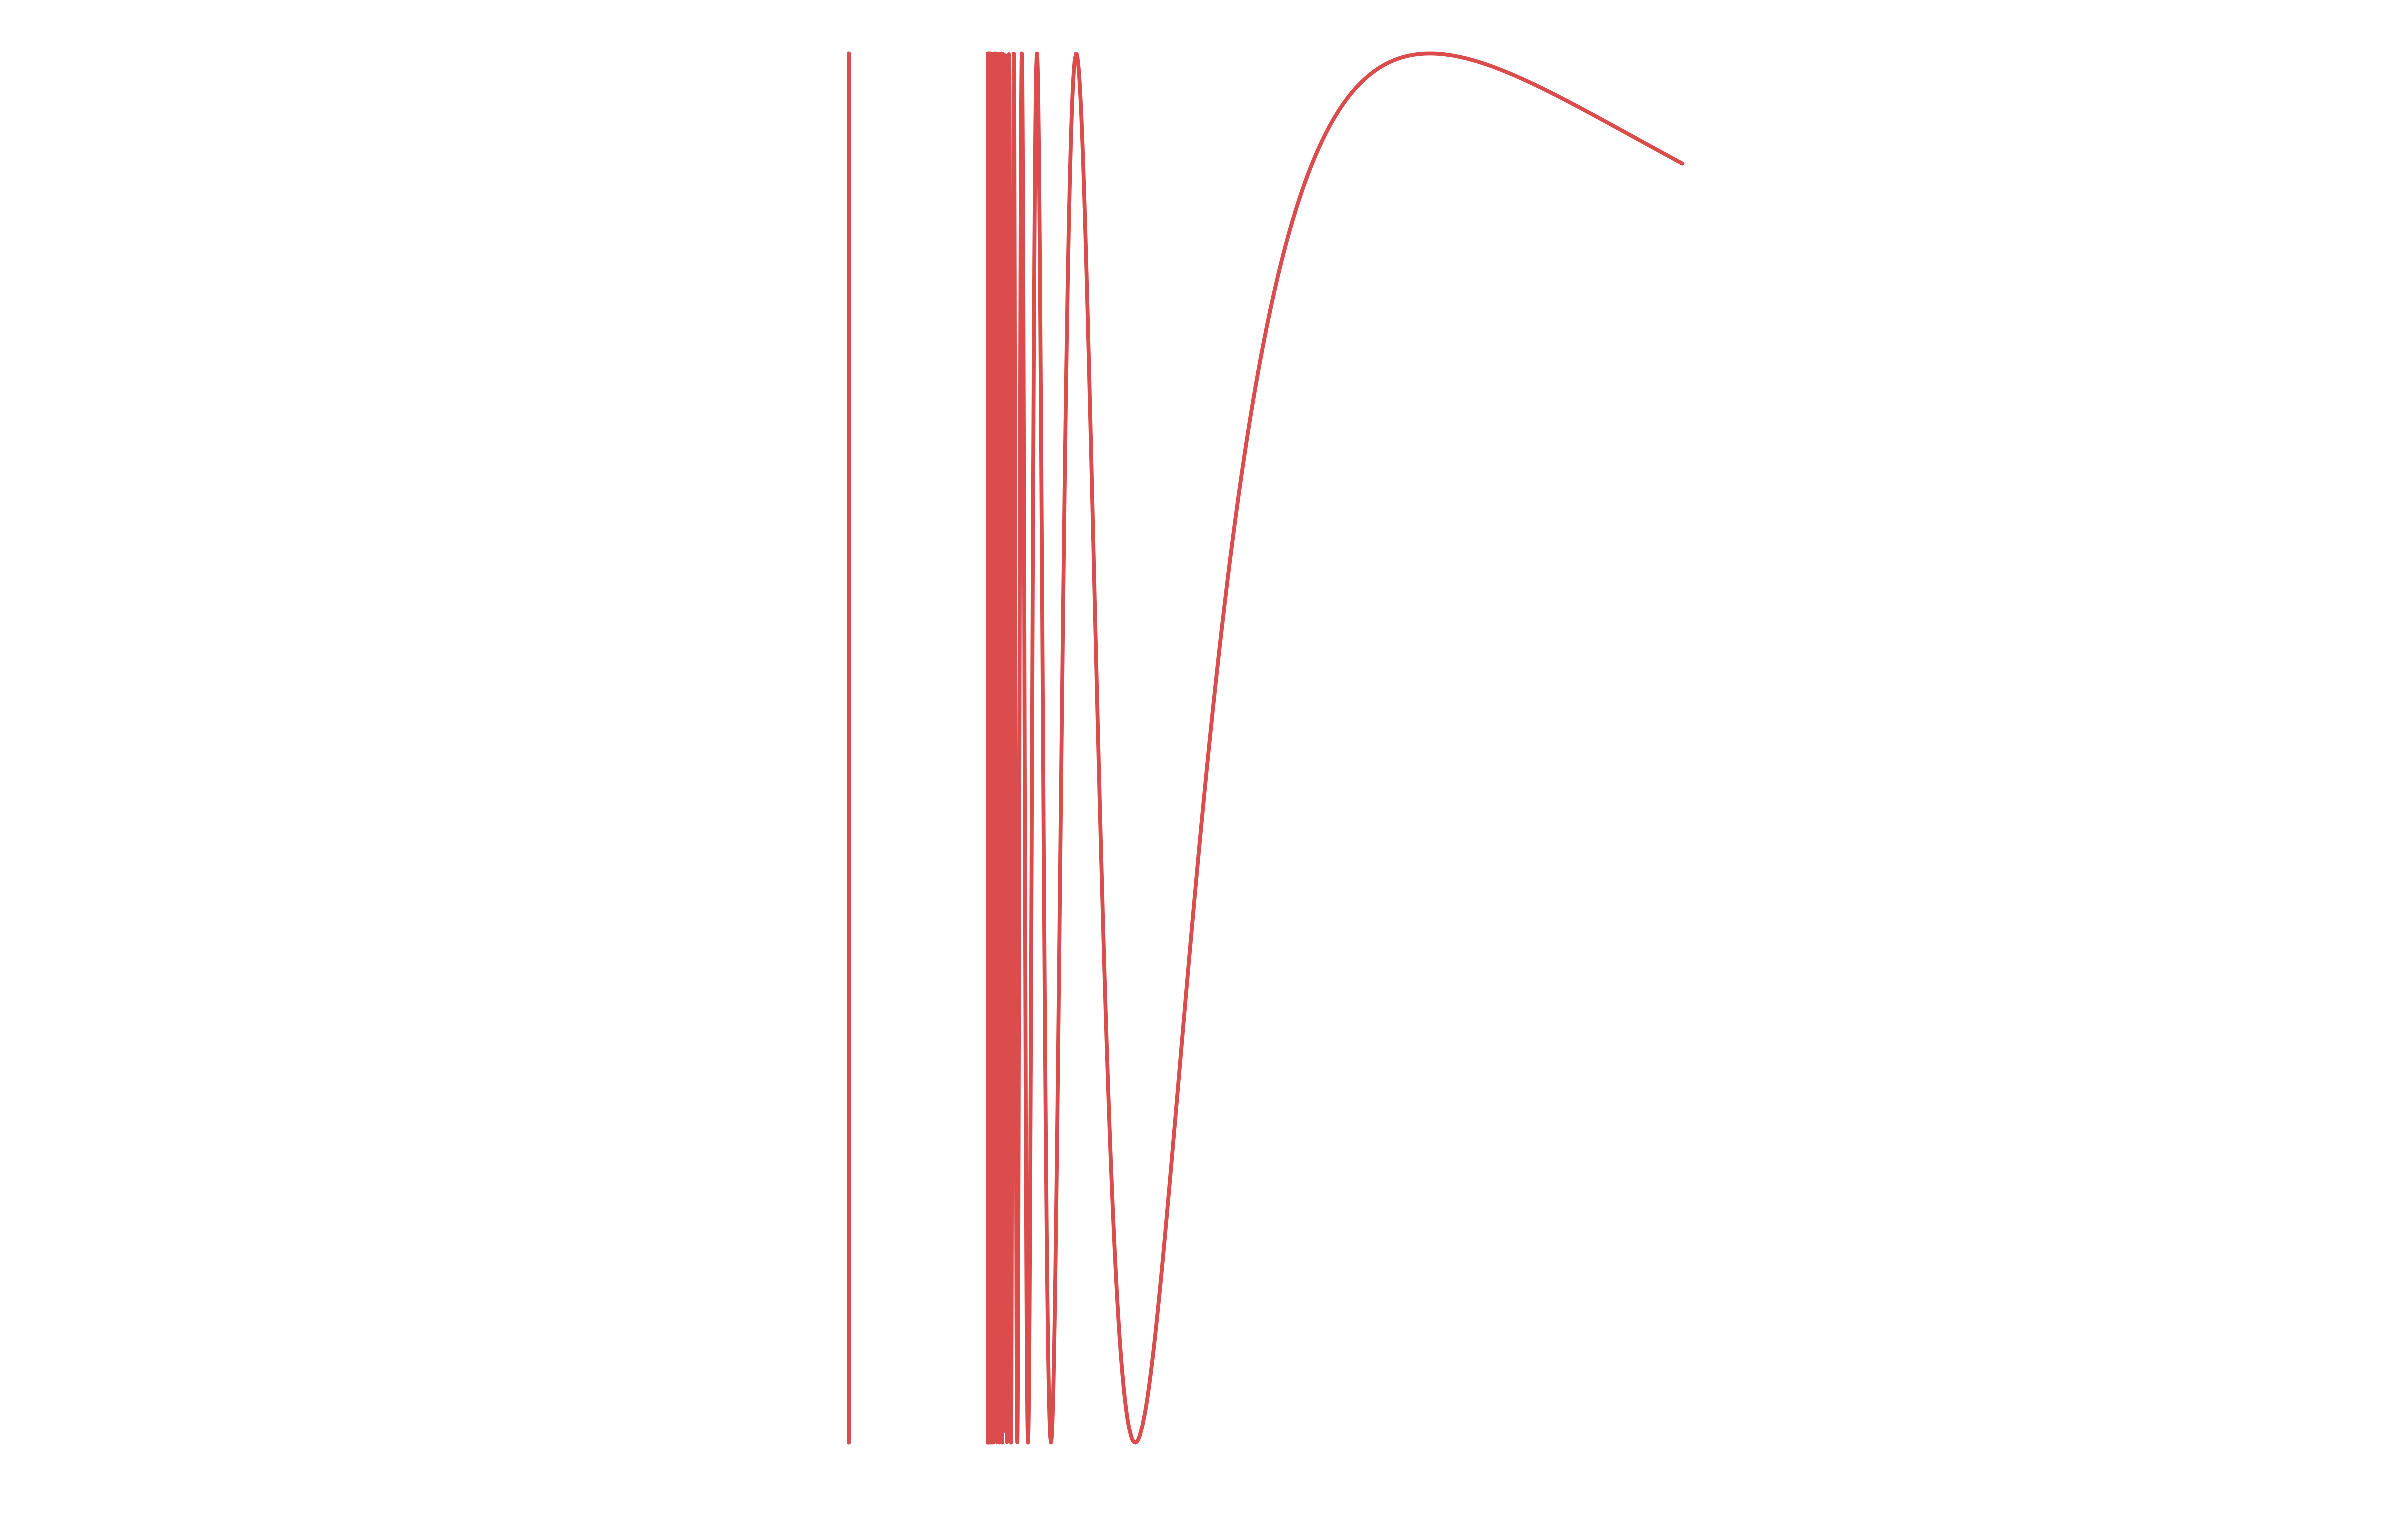
\includegraphics[scale = 0.2]{Figures/Chapter3/topologistsSineCurve.eps}
            \caption{The topologists Sine Curve, defined by $x \times \sin{\frac{1}{x}}$.}
            \label{fig_3.2}
        \end{figure}

        Let $S=\{x \times \sin{\frac{1}{x}}:0 < x \leq 1\}$. This is the image of the continuous map
        $x \rightarrow x \times \sin{\frac{1}{x}$ from $(0,1] \rightarrow \R^2$, Since $(0,1]$ is
            connected, then so is $S$. by theorem \ref{3.1.6}. We call $\cl{S}=S \cup (0 \times
            [-1,1])$ the \textbf{topologist's sine curve} (see figure \ref{fig_3.2}).

            Suppose that $f:[a,c] \rightarrow \cl{S}$ is a path begining at $0$ and ending at a
            point in  $S$. The set  $T=\{t \in \R:f(t) \in 0 \times [-1,1]\}$ is closed, so it has a
            largest element $b$. Then  $f$ is a path mapping  $b \rightarrow 0 \times [-1,1]$ and
            taking all other points to $S$. Suppose that  $[b,c]=[0,1]$ and let $f(t)=(x(t),y(t))$
            where $x(0)=0$, $x(t)>0$ and $y(t)=\sin{\frac{1}{x(t)}}$ for all $t>0$. For  $n \in
            \Z^+$, choose  $0<u<x(\frac{1}{n})$ such that $\sin{\frac{1}{u}}=(-1)^n$. By the
            intermediate value theorem, there are $0<t_n<\frac{1}{n}$ with $x(t_n)=u$. Then the
            sequence $\{t_n\} \rightarrow 0$, and $x(t_n)=(-1)^n$, which diverges; a contradiciton
            since $x(0)=0$ and $\{t_n\} \rightarrow 0$. Hence $\cl{S}$ is not path connected.

    \end{enumerate}
\end{example} 

\section{Outer Measures}

\begin{definition}
    Let $X$ be a set. An \textbf{outer-measure} on $X$ is a function $m^\ast:2^X
    \xrightarrow{} [0, \infty)$ for which the following are true:
    \begin{enumerate}
        \item[(1)] $m^\ast(\emptyset)=0$.

        \item[(2)] If $A \subseteq B$, then $m^\ast(A) \leq m^\ast(B)$.

        \item[(3)] If $\{A_n\}$ is a countable collection of subsets of $X$,
            then
            \begin{equation*}
                m^\ast\Big{(} \bigcup{A_n} \Big{)} \leq \sum{m^\ast(A_n)}
            \end{equation*}
    \end{enumerate}
\end{definition}

\begin{lemma}\label{lemma_1.3.1}
    Let $X$ be a set, and  $\Ec$ a collection of subsets of $X$ for which
    $\emtyset \in \Ec$ and $X \in \Ec$, and let $l:\Ec \xrightarrow{} [0, \infty]$
    a function for which $l(\emptyset)=0$. For any $A \subseteq X$, define
    \begin{equation}\label{equation_1.4}
        m^\ast(A)=\inf{\Big{\{} \sum{l(E_n)} : E_n \in \Ec, \text{ and }
       A \subseteq \bigcup{E_n} \Big{\}}}
    \end{equation}
    Then $m^\ast$ defines an outer-measure.
\end{lemma}
\begin{proof}
    For all $A \subseteq X$, there is a collection $\{E_n\}$ of sets of $\Ec$
    for which $A \subseteq \bigcup{E_n}$. Observe first, that since $l(E_n) \geq
    0$ for all $n$, that  $\sum{l(E_n)} \geq 0$. This makes $m^\ast(A) \geq 0$.
    Now, choose $E_n=\emptyset$ for all  $n$, and we get  $m^\ast(\emptyset)=0$.

    Now, let $A \subseteq B$ subsets of $X$, and let  $\{E_n\}$ a countable
    cover of $B$. Then  $\{E_n\}$ is also a countable cover of $A$. Define then
     $E=\{\sum{l(E_n)} : A \subseteq \bigcup{E_n}\}$ and $F=\{\sum{l(E_n)} :
     B \subseteq \bigcup{E_n}\}$. Since $A \subseteq B$, $F \subseteq E$.
     Therefore, by least upper bounds, we have $\inf{F} \leq \inf{B}$, that is
     $m^\ast(A) \leq m^\ast(B)$.

     Lastly, let $\{A_n\}$ be a countable collection of sets of $X$, and let
     $A=\bigcup{A_n}$. Now, if at least one of the $m(A_n)=\infty$, then we are
     done. Suppose then that $m(A_n)<\infty$ for all $n$. Now, there exists a
     cover of  $A_n$,  $\{E_{n,k}\}_k$ for which
     \begin{equation*}
         \sum_{k}{l(E_{n,k})}<m^\ast(A)+\frac{1}{2^k}
     \end{equation*}
     consider now the countable collection
     $\{E_{n,k}\}_{n,k}=\bigcup_{n}{\{E_{n,k}\}_k}$. Then $\{E_{n,k}\}_{n,k}$ is
     a countable cover for $A$, and we get
     \begin{equation*}
         m^\ast(A) \leq \sum_n{\sum_k{l(E_{n,k})}}<
         \sum_n{m^\ast(A_n)+\frac{1}{2^k}}=\sum_n{m^\ast(A_n)}+\e
     \end{equation*}
     Take then $\e>0$ small, and we get the result.
\end{proof}
\begin{corollary}
    If $E$ is a set of $\Ec$, then $m^\ast(E)=l(E)$.
\end{corollary}
\begin{proof}
    Observe that $E$ covers itself, so that
    $m^\ast(E)=\inf{\{\sum_{i=1}^1{E}\}}=\inf{l(E)}=l(E)$.
\end{proof}

\begin{definition}
    Let $X$ be a set. We call a subset $A$ of  $X$  \textbf{$m^\ast$-measurable}
    if for any subset $E$ of  $X$,
    \begin{equation}\label{equation_1.5}
        m^\ast(E)=m^\ast(E \cap A)+m^\ast(E \cap \com{X}{A})
    \end{equation}
\end{definition}

\begin{lemma}\label{lemma_1.3.2}
    Let $X$ be a set. A subset $A$ of $X$ is  $m^\ast$-measurable if, and only
    if
    \begin{equation*}
        m^\ast(E) \geq m^\ast(E \cap A)+m^\ast(E \cap \com{X}{A}) \text{ for all }
        E \subseteq X
    \end{equation*}
\end{lemma}

\begin{theorem}[Carath\'eodory's Theorem]\label{theorem_1.3.3}
    Let $X$ be a set, and $m^\ast$ an outer-measure on $X$. Then the collection
    of all $m^\ast$-measurable sets forms a  $\s$-algebra. Moreover,  $m^\ast$
    is a complete measure on this $\s$-algebra.
\end{theorem}
\begin{proof}
    Let $\Mc$ be the collection of all  $m^\ast$-measurable sets. Observe first
    that if  $A \in \Mc$, then so is $\com{X}{A}$, by symetry of equation
    \ref{equation_1.5}. So $\Mc$ is closed under complements. Now, let  $A,B \in
    \Mc$. Then we have
    \begin{align*}
        m^\ast(E) &= m^\ast(E \cap A)+m^\ast(E \cap \com{X}{A}) \\
               &= m^\ast(E \cap A \cap B)+m^\ast(E \cap A \cap \com{X}{B})
                        +m^\ast(E \cap B \cap \com{X}{A})+m^\ast(E \cap
                        \com{X}{A} \cap \com{X}{B}) \\
    \end{align*}
    Now, since $A \cup B=(A \cap B) \cup (A \cap \com{X}{B}) \cup (B \cap
    \com{X}{A})$, so by subadditivity, we get
    \begin{equation*}
        m^\ast(E \cap A \cap B)+m^\ast(E \cap A \cap \com{X}{B})+m^\ast(E \cap
        \com{X}{A} \cap B) \geq m^\ast(E \cap (A \cup B))
    \end{equation*}
    i.e. $m^\ast(E) \geq m^\ast(E \cap (A \cup B))+m^\ast(E \cap \com{X}{(A \cup
    B)})$. That is, $A \cup B \in \Mc$, making $\Mc$ an algebra.

    Now, let  $\{A_n\}$ be a countable disjoint collection of
    $m^\ast$-measurable sets, and take  $B_n=\bigcup_{i=1}^n{A_i}$, and take
    $B=\bigcup{B_n}$. Then for all $E \subseteq X$
    \begin{align*}
        m^\ast(E \cap B_n) &= m^\ast(E \cap B_n \cap A_n)+m^\ast(E \cap B_n \cap
                        \com{X}{A_n}) \\
                     &= m^\ast(E \ca A_n)+m^\ast(E \cap B_{n-1})
    \end{align*}
    an induction argument on the collection $\{B_n\}$ gives us
    \begin{equation*}
        m^\ast(E \cap B_n)=\sum_{i=1}^n{m^\ast(E \cap A_i)}
    \end{equation*}
    therefore
    \begin{equation*}
        m^\ast(E)=m^\ast(E \cap B_n)+m^\ast(E \cap \com{X}{B_n}) \geq
        \sum_{i=1}^n{m^\at(E \cap A_i)}+m^\ast(E \cap \com{X}{B_n})
    \end{equation*}
    letting $n \xrightarrow{} \infty$,
    \begin{equation*}
        m^\ast(E) \geq \sum{m^\at(E \cap A_n)}+m^\ast(E \cap \com{X}{B_n})
    \end{equation*}
    so that $B \in \Mc$. Taking $E=B$, we get  $m^\ast(B)=\sum{m^\ast(A_n)}$ so
    that $m^\ast$ is countably additive, and $\Mc$ is a $\s$-algebra.

    Finally, let $m^\ast(A)=0$, then for any $E \subseteq X$, we have
    \begin{equation*}
        m^\ast(E) \leq m^\ast(E \cap A)+m^\ast(E \cap \com{X}{A})=
        m^\ast(E \cap \com{X}{A}) \leq m^\ast(E)
    \end{equation*}
    so that $A \in \Mc$, which makes $m^\ast$ complete on $\Mc$.
\end{proof}

\begin{definition}
    Let $X$ be a set, and  $\Ac$ an algebra on  $X$. We define a
    \textbf{pre-measure} on $\Ac$ to be a function  $m_0:\Ac \xrightarrow{}
    [0,\infty]$ for which
    \begin{enumerate}
        \item[(1)] $m_0(\emptyset)=0$.

        \item[(2)] If $\{A_n\}$ is a countably disjoint collection of sets in
            $\Ac$, for which  $\bigcup{A_n} \in \Ac$, then
            \begin{equation}\label{equation_1.6}
                m_0\Big{(} \bigcup{A_n} \Big{)}=\sum{m_0(A_n)}
            \end{equation}
    \end{enumerate}
\end{definition}

\begin{lemma}\label{lemma_1.3.4}
    Pre-measures on algebras define outer-measures on the overlying sets.
\end{lemma}
\begin{proof}
    Consider the definition of the outer measure $m^\ast$ from equation
    \ref{equation_1.4}, simply take $l=m_0$, and $\Ec=\Ac$.
\end{proof}

\begin{lemma}\label{lemma_1.3.5}
    Let $X$ be a set, and  $\Ac$ an algebra on  $X$. If  $m_0$ is pre-measure on
    $\Ac$, and the measure $m^\ast$ is define by
    \begin{equation*}
        m^\ast(A)=\inf{\Big{\{} \sum{m_0(E_n)} : E_n \in \Ac, \text{ and }
       A \subseteq \bigcup{E_n} \Big{\}}}
    \end{equation*}
    then the following are true.
    \begin{enumerate}
        \item[(1)] $m_0=m^\ast$ on $\Ac$.

        \item[(2)] Every set in $\Ac$ is  $m^\ast$-measurable.
    \end{enumerate}
\end{lemma}
\begin{proof}
    For (1), suppose that $A \in \Ac$, and that $A \subseteq \bigcup{E_n}$ for
    $E_n \in \Ac$. Take
    \begin{equation*}
        F_n=A \cap \com{A_n}{\Big{(} \bigcup_{i=1}^{n-1}{A_i} \Big{)}}
    \end{equation*}
    then $\{F_n\}$ is a disjoint countable collection of sets of $\Ac$ for which
     $A=\bigcup{F_n}$. Hence
     \begin{equation*}
         mo(A)=\sum{m_0(F_n)} \leq \sum{m_0(E_n)}
     \end{equation*}
     it follows from hypothesis that $m_0(A) \leq m^\ast(E)$. For the reverse
     inclusion, simply take $A \subseteq \bigcup{E_n}$ with $A=E_1$ and
     $E_n=\emptyset$ for all  $n>1$.

     For (2), if $A \in \Ac$, and $E \subseteq X$, and $\e>0$, there is a
     collection  $\{B_n\}$ of sets of $\Ac$ with  $A \subseteq \bigcup{B_n}$,
     and
     \begin{equation*}
         \sum{m_0(B_n)}<m^\ast(A)+\e
     \end{equation*}
     by additivity of $m_0$ on $\Ac$, we get
     \begin{equation*}
         m^\ast(E)+\e \geq \sum{m_0(B_n \cap A)}+\sum{m_0(B_n \cap \com{X}{A})}
                    \geq m^\ast(E \cap A)+m^\ast(E \cap \com{X}{A})
     \end{equation*}
\end{proof}

\begin{theorem}\label{theorem_1.3.6}
    Let $X$ be a set, and  $\Ac$ an algerba on  $X$. Let  $m_0$ be a pre-measure
    on $\Ac$, and let  $\Mc$ the  $\s$-algebra generated by  $\Ac$. Then there
    exists a measure  $m$ on  $\Mc$ whose restriction to  $\AC$ is  $m_0$.
    Moreover, if $n$ is another measure extending from $m_0$, then
    \begin{equation*}
        n(E) \leq m(E) \text{ for all } E \in \Mc
    \end{equation*}
    where equality holds when $m(E)<\infty$. Lastly, if $m_0$ is $\s$-finite,
    then  $m$ is the unique extension of  $m_0$ to $\Mc$.
\end{theorem}
\begin{proof}
    Define again,
    \begin{equation*}
        m^\ast(A)=\inf{\Big{\{} \sum{m_0(E_k)} : E_k \in \Ac, \text{ and }
       A \subseteq \bigcup{E_k} \Big{\}}}
    \end{equation*}
    then by Carath\'eodory's theorem, lemma \ref{lemma_1.3.5}, the first result
    follows, since the $\s$-algebra of all  $m^\ast$-measurable sets contains
    $\Ac$, and as consequence, also contains $\Mc$.

    Now, let $E \in \Mc$ with $E \subseteq \bigcup{A_k}$, where $A_k \in \Ac$.
    Then
    \begin{equation*}
        n(E) \leq \sum{n(A_n)}=\sum{m_0(A_n)}
    \end{equation*}
    which gives us $n(E) \leq m(E)$. Now, set $A=\bigcup{A_n}$, and observe that
    \begin{equation*}
        n(A)=\lim_{k \xrightarrow{} \infty}{n\Big{(} \bigcup_{i=1}^k{A_i} \Big{)}}
        =\lim_{k \xrightarrow{} \infty}{m\Big{(} \bigcup_{i=1}^k{A_i}
        \Big{)}}=m(A)
    \end{equation*}
    if $m(E)<\infty$, choose $A_k$ such that  $m(A)<m(E)+\e$ for $\e>0$. Then
    $m(\com{A}{E})<\e$, and
    \begin{equation*}
        m(E) \leq m(A)=n(A)=n(E)+n(\com{A}{E}) \leq n(E)+m(\com{A}{E}) \leq
        n(E)+\e
    \end{equation*}
    taking $\e$ small, we get $n(E)=m(E)$.

    Finally, suppose that $m_0$ is $\s$-finite, and let $X=\bigcup{A_k}$ for
    s me0disjoint collection $\ A_n\}$, then $ m_0 m_0)<\infty$. Then for every
    $E \in \Mc$,
    \begin{equation*}
        m(E)=\sum{m(E \cap A_k)}=\sum{n(E \cap A_k)}=n(E)
    \end{equation*}
    so that $m=n$, making $m$ unique.
\end{proof}

\section{Roots of Analytic Functions}

%----------------------------------------------------------------------------------------
%	SECTION 1.1
%----------------------------------------------------------------------------------------

\section{Rectifiable Curves.}

\begin{definition}
    We call a continuous mapping $\gamma:[a,b] \rightarrow \R^k$ a
    \textbf{curve} in $\R^k$, on  an interval $[a,b]$. If  $\gamma$ is 1-1, we
    call the curve an \textbf{arc}, and we call  $\gamma$ a \textbf{closed
    curve} if  $\gamma(a)=\gamma(b)$.

    Now, for each partition $P$ of  $[a,b]$, and for  $\gamma$ a curve on
    $[a,b]$, and let:
        \begin{equation}
            \Lambda(\gamma,P)=\sum_{i=1}^{n}{||\gamma(x_i)-\gamma(x_{i-1})||}		
        \end{equation}
    We deefine the \textbf{length} of $\gamma$ to be :
        \begin{equation}
            \Lambda(\gamma)=\sup_{P}{\Lambda(\gamma,P)}		
        \end{equation} 
        If $\gamma$ is of finite length  (i.e. $\Lambda(\gamma)<\infty$), then
        we call $\gamma$ a \textbf{rectifiable} curve.
\end{definition}

\begin{theorem}\label{7.5.1}
    Let $\gamma$ be a differentiable curve on  $[a,b]$, if  $\gamma'$ is
    continuous, then  $\gamma$ is rectifiable and
        \begin{equation}
            \Lambda(\gamma)=\int_{a}^{b}{||\gamma'|| dt}		
        \end{equation} 
\end{theorem}
\begin{proof}
    If $a \leq x_{i-1}<x_i \leq b$, then
    $||\gamma(x_i)-\gamma(x_{i-1})||=||\int_{x_{i-1}}^{x_i}{\gamma' dt}|| \leq
    \int_{x_{i-1}}^{x_i}{||\gamma'|| dt}$, by the Fundamental theorem of
    calculus, thus $\Lambda(\gamma,P) \leq \int_{a}^{b}{||\gamma'|| dt}$ 
    for every partition $P$ of  $[a,b]$, then cinsequently, we have
    $\Lambda(\gamma)=\int{||\gamma'|| dt}$. Consequently, $\gamma$ is
    rectifiable.

    Now let  $\epsilon>0$, since  $\gamma'$ is uniformly continuous on  $[a,b]$,
    there is a  $\delta>0$ such that  $||\gamma'(s)-\gamma'(t)||<\epsilon$
    whenever  $|s-y|<\delta$ for  $s,t \in [a,b]$. Let $P$ be a partition of
    $[a,b]$, with  $\Delta{x_i}<\delta$ for all  $i$, and it  $x_{i-1} \leq t
    \leq x_i$, we have  $||\gamma'(t)|| \leq ||\gamma'(x_i)||+\epsilon$, hence:
        \begin{align*}
            \int_{x_{i-1}}^{x_i}{||\gamma'||\Delta{x_i}} &\leq ||\gamma'(x_i)||\Delta{x_i}+\epsilon\Delta{x_i} \\ 
                &= ||\int_{x_{i-1}}^{x_i}{(\gamma'(t)+\gamma'(x_i)-\gamma'(t))}||+\epsilon\Delta{x_i} \\
                &\leq ||\int_{x_{i-1}}^{x_i}{\gamma' dt}||+||\int_{x_{i-1}}^{x_i}{(\gamma'(x_i)-\gamma'(t)) dt}||+\epsilon\Delta{x_i} \\
                & \leq ||\gamma(x_i)-\gamma(x_{i-1})||+2\epsilon\Delta{x_i} \\
        \end{align*}
    Thus, $\int_{a}^{b}{||\gamma'|| dt} \leq \Lambda(\gamma,P)+2\epsilon(b-a)$, 
    so for  $\epsilon$ small enough, we get that  $\int{||\gamma'||} \leq \Lambda(\gamma)$.
\end{proof}

\section{Gr\"obner Bases}
\label{section_7.6}

\begin{definition}
  Let $R$ be a Noetherian ring, and $\leq$ a monomial ordering on
  $R[x_1, \dots, x_n]$. We define the \textbf{leading term} of a
  polynomial $f(x_1, \dots, x_n)$ to be the maximum element of the
  ideal $(f)$, and denote it $LT(f)$. If $\af$ is an ideal in $R[x_1,
  \dots, x_n]$, then we define the \textbf{ideal of leading terms} of
  $\af$ to be the ideal generated by all leading terms of polynomials
  of $\af$; i.e.
  \begin{equation*}
    LT(\af)=(LT(f) : f \in \af)
  \end{equation*}
  If $\af=(f_1, \dots, f_m)$, we write $LT(f_1, \dots, f_m)$. If
  $\af=(f)$, we keep the previous convention $LT(\af)$.
\end{definition}

\begin{definition}
  Let $f(x_1, \dots, x_n)$ a multi-variate polynomial over a
  Noetherian ring. We define the \textbf{multi-degree} of $f$ to be
  the multi-degree of $LT(f)$, and we denote it $\partial{f}$.
\end{definition}

\begin{proposition}\label{proposition_7.6.1}
  Let $f_1, \dots, f_m$ be multivariate polynomials over a Noetherian
  ring. Then
  \begin{equation*}
    (LT(f_1), \dots, LT(f_m)) \subseteq LT(f_1, \dots, f_m)
  \end{equation*}
\end{proposition}
\begin{proof}
  Observe that since $f_i \in \af$ for each $1 \leq i \leq m$, then
  $LT(f_i) \in LT(\af)$ for each $1 \leq i \leq m$.
\end{proof}

\begin{proposition}\label{proposition_7.6.2}
  Let $k$ be field, and $f,g \in k[x_1, \dots, x_n]$. Then
  the following are true:
  \begin{enumerate}
    \item[(1)] $LT(fg)=LT(f)LT(g)$.

    \item[(2)] $LT(f+g) \leq \max{\{LT(f), LT(g)\}}$ with equality
      holding if $LT(f) \neq LT(g)$.
  \end{enumerate}
\end{proposition}
\begin{proof}
  Let $AX^\a=LT(f)$ and $BX^\b=LT(g)$, and make the convention $f(x_1,
  \dots, x_n)=f(X)$. Then we have for some $h,h' \in R[x_1, \dots,
  x_n]$ that $f(X)=AX^\a+h(X)$ and $g=BX^\b+h'(X)$. Then
  \begin{align*}
    fg(X) &=  (AX^\a+h(X))(BX^\b+h'(X))  \\
          &= (AB)X^\a X^\b+(AX^\a h'(X)+BX^\b h(X)+h(X)h'(X))  \\
          &=  (AB)X^{\a+\b}+h''(X)  \\
  \end{align*}
  so that $LT(fg)=LT(f)LT(g)$.

  Now, we also observe that
  \begin{equation*}
    f+g(X)=(AX^\a+BX^\b)+(h(X)+h'(X))
  \end{equation*}
  if $\a=\b$, and $B=-A$, then $f+g(X)=h(X)+h'(X)$ and $LT(f+g)<AX^\a$
  and $LT(f+g)<BX^\b$, so that $LT(f+g)<\max{\{AX^\a,BX^\b\}}$. Now, we have
  if  $\a \neq \b$, then
  \begin{align*}
    f+g(X)=AX^\a+(BX^\b+h(X)+h'(X))  & \text{ if } \b < \a  \\
    f+g(X)=AX^\b+(BX^\a+h(X)+h'(X))  & \text{ if } \a < \b  \\
  \end{align*}
  in either case either $LT(f+g)=\max{\{X^\a,X^\b\}}$.
\end{proof}
\begin{corollary}
  The following are true:
  \begin{enumerate}
    \item[(1)] $\partial{(fg)}=\partial{f}+\partial{g}$.

    \item[(2)] $\partial{(f+g)} \leq \max{\{\partial{f},
      \partial{g}\}}$, with equality holding if $\partial{f} \neq
      \partial{g}$.
  \end{enumerate}
\end{corollary}

\begin{proposition}\label{proposition_7.6.3}
  Let $R$ be a Noetherian ring. Let $\af=(X^{\a_1}, \dots, X^{\a_m})$ in $R[x_1,
  \dots x_n]$ and ideal and $f \in R[x_1, \dots, x_n]$. Then $f \in
  \af$ if, and only if each monomial term of $f$ is a multiple of some
  monomial  $X^\a_i$ generating $\af$.
\end{proposition}
\begin{proof}
  Suppose that $f \in \af$. Then
  \begin{equation*}
    f(x_1, \dots, x_n)=f(X)=\sum_{i=1}^m{A_mX^{\a_i}}
  \end{equation*}
  and notice that each monomial $X^{\a_i}$ is a multiple of itself.

  Conversely suppose that
  \begin{equation*}
    f(X)=\sum_{j=1}^n{A_jX^{\b_j}}
  \end{equation*}
  and that there is an $X^{\a_i}$ for which $X^{\a_i}|X^{\b_j}$ for
  all $1 \leq j \leq n$. Then $X^{\b_j} \in (X^{\a_i}) \subseteq
  (X^{\a_1}, \dots, X^{\a_m})$. Then $f \in \af$.
\end{proof}

\begin{example}\label{example_7.8}
  Let $k$ be a field.
  \begin{enumerate}
    \item[(1)] Choose the lexicographic order $x>y$ on $k[x,y]$. Let
      $f(x,y)=x^3y-xy^2+1$ and $g(x,y)=-y^3+x^2y^2-1$. Then
      $LT(f)=x^3y$ with $\partial{f}=(3,1)$, and $LT(g)=x^2y^2$ with
      $\partial{g}=(2,2)$. Then
      \begin{align*}
        LT(fg)=x^5y^3 & \text{ and } \partial{(fg)}=(5,3) \\
        LT(f+g)=x^3y  & \text{ and } \partial{(f+g)}=(3,0)  \\
      \end{align*}
      Now, take $\af=(f,g)$, then $(x^3y,x^2y^2) \subseteq LT(f,g)$.
      However, observe that $yf(x,y)-xg(x,y)=x+y \in \af$, and
      $LT(yf+xg)=x \in LT(f,g)$. However $x \notin
      (x^3y,x^2y^2)$. That is, in general, if $\af=(f_1,
      \dots, f_m)$, then $LT(f_1, \dots, f_m) \neq (LT(f_1), \dots
      LT(f_m))$.

    \item[(2)] Choose the lexicographic ordering $y>x$ in  $k[x,y]$.
      Let again $f(x,y)=x^3y-xy^2+1$ and $g(x,y)=-y^3+x^2y^2-1$. Then
      $LT(f)=xy^2$ with $\partial{f}=(1,2)$ and $LT(g)=y^3$ with
      $\partial{g}=(0,3)$. Then
      \begin{align*}
        LT(fg)=xy^5 & \text{ and } \partial{(fg)}=(1,5) \\
        LT(f+g)=-y^3 & \text{ and } \partial{(f+g)}=(03) \\
      \end{align*}
      Again, we have $(xy^2, y^3) \subseteq LT(f,g)$, but $LT(f,g)
      \neq (xy^2,y^3)$. We observe that $y \in LT(f,g)$ but $y \notin
      (xy^2,y^3)$.

    \item[(3)] Choose any order on $k[x,y]$, and let $f(x,y) \neq 0$.
      Let $\af=(f)$, then $LT(\af)=(LT(f))$, since every monomial term
      of $f$ is a multiple of  $LT(f)$.
  \end{enumerate}
\end{example}

\begin{definition}
  Let $k$ be a field, and $\af$ an ideal of $k[x_1, \dots, x_n]$. We
  call a finite set of generators $G=\{g_1, \dots, g_m\}$ of $\af$ a
  \textbf{Gr\"obner basis} for $\af$ if
  \begin{equation*}
    LT(\af)=(LT(g_1), \dots, LT(g_m))
  \end{equation*}
\end{definition}

\section{Cyclotomic Polynomials}
\label{section_8.7}

\begin{definition}
  We define \textbf{Euler's totient} to be the map $\phi:\Z \xrightarrow{} \Z$
  defined by the rule $\phi(n)=|\{a \in \Z : (a,n)=1\}|$. That is, $\phi$
  of  $n$ is the number of all integers less than  $n$, coprime to  $n$.
\end{definition}

\begin{definition}
  We define $\Xi_n$ to be the \textbf{group of all primitive $n$-th roots of
  unity}, $\xi$ for which  $\xi^n=1$.
\end{definition}

\begin{lemma}\label{lemma_8.7.1}
  $\Xi_n \simeq \faktor{\Z}{n\Z}$.
\end{lemma}
\begin{proof}
  The map $a \xrightarrow{} \xi^a$ defines the required isomorphism.
\end{proof}
\begin{corollary}
  $\ord{\Xi_n}=\phi(n)$ where $\phi$ is Euler's totient.
\end{corollary}
\begin{proof}
  Since $\xi^n \equiv \xi^{0 \mod{n}} \equiv 1$, we have every non identity
  power of $\xi$ has exponenct coprime to  $n$. That is there are $\phi(n)$
  such distinct powers of$\xi$.
\end{proof}
\begin{corollary}
  If $d|n$, then  $\Xi_d \leq \Xi_n$.
\end{corollary}
\begin{proof}
  Notice that if $d|n$, then $d=mn$ for some  $m \in \Z^+$. Then $\xi^d=1$
  implies  $(\xi^d)=\xi^{dm}=\xi^n=1$.
\end{proof}

\begin{definition}
  We define the \textbf{$n$-th cyclotomic polynomial} to be the polynomial
  \begin{equation*}
    \Phi_n(x)=\prod{x-\xi}
  \end{equation*}
  having as roots all $n$-primitive roots of unity.
\end{definition}

\begin{lemma}\label{lemma_8.7.2}
  The $n$-th cyclotomic polynomial  $\Phi_n$ has degree
  $\deg{\Phi_n}=\phi(n)$, where $\phi$ is Euler's totient.
\end{lemma}
\begin{proof}
  Recall that $\ord{\Xi_n}=\phi(n)$, and since the elements of $\Xi_n$ are the
  roots of  $\Phi_n$, there are  $\phi(n)$ such roots. This puts
  $\deg{\Phi_n}=\phi(n)$.
\end{proof}

\begin{example}[Computing Cyclotomic Polynomials]\label{8.18}
  Recall that the polynomial $x^n-1$ has as roots precisely all  $n$-th roots
  of unity  $\xi$, that is $\xi^n=1$. If $x^n-1 \in F[x]$, $F$ a field, the
  the splitting field of  $x^n-1$ is  $F(\xi)$. Then we have
  \begin{equation*}
    x^n-1=\prod_{\xi \in \Xi_n}{(x-\xi)}
  \end{equation*}
  Now, grouping those factors where $\xi^d=1$ for some  $d|n$, then we have
  \begin{equation*}
    x^n-1=\prod_{\xi \in \Xi_d}{(x-\xi)}\prod_{\xi \in \Xi_n}{(x-\xi)}=
    \prod{d|n}{\prod_{\xi \in \Xi_n}{(x-\xi)}}=\prod_{d|n}{\Phi_n(x)}
  \end{equation*}
  that is,
  \begin{equation*}
    x^n-1=\prod_{d|n}{\Phi_d(x)}
  \end{equation*}
  which gives a method for computing $\Phi_n$ recursively.

  We have  $\Phi_1(x)=x-1$ and $\Phi_2(x)=x+1$. Now,
  $\Phi_3(x)=\Phi_1(x)\Phi_3(x)=(x-1)\Phi_3(x)$, so that
  \begin{equation*}
    Phi_n(x)=x^2+x+1
  \end{equation*}
  We have
  $\Phi_4(x)=\Phi_1(x)\Phi_2(x)\Phi_4(x)=(x-1)(x+1)\Phi_4(x)=(x^2-1)\Phi_4(x)$.
  So
  \begin{equation*}
    \Phi_4(x)=x^2+1
  \end{equation*}
  Similarly,
  \begin{align*}
    \Phi_5(x)   &=  x^4+x^3+x+1 \\
    \Phi_6(x)   &=  x^2-x+1 \\
    \Phi_7(x)   &=  x^6+x^5+x^4+x^3+x^2+x+1 \\
    \Phi_8(x)   &= x^4+1    \\
    \Phi_9(x)   &=  x^6+x^x+1   \\
    \Phi_{10}(x)   &=   x^4-x^3+x^2-x+1 \\
    \Phi_{11}(x)   &=   x^{10}+x^9+x^8+x^7+x^6+x^5+x^4+x^3+x^2+x+1  \\
    \Phi_{12}(x)   &=   x^4-x^2+1   \\
  \end{align*}
  Also observe that if $p$ is prime, then
  \begin{equation*}
    \Phi_p(x)=\sum_{i=0}^{p-1}{x^i}=x^{p-1}+x^p+\dots+x+1
  \end{equation*}
\end{example}

\begin{lemma}\label{lemma_8.7.3}
  $\Phi_n(x)$ is monic over $\Z$.
\end{lemma}
\begin{proof}
  Notice that since $x^n-1=\prod{\Phi_d(x)}$, is monic, then each $\Phi_d$
  must also be monic for all  $d|n$.

  Now, by induction on $n$, for  $n=1$, it is clear that  $x-1$ has
  coefficiencts in  $\Z$  (if $x^n-1 \in \Z[x]$ we are done, if not, just take
  $1_F \xrightarrow{} 1_\Z$, whre $F$ is the underlying field of  $x^n-1$).
  Now, suppose that $\Phi_d(x) \in \Z[x]$ for all $1 \leq d <n$, and  $d|n$.
  Then  $x^n-1=f(x)\Phi_n(x)$, where $f(x)=\prod{\Phi_d(x)}$ is monic over
  $\Z$. Moreover,  $f|x^n-1$, in the splitting field $\Q(\xi)$ (since we take
  $1_F \xrightarrow{} F_\Z$), where $\xi^n=1$. Then  $f|x^n-1$ over  $\Q$ by
  the division theorem, and by Gauss' lemma, $f|x^n-1$ in $\Z$. So $\Phi_n \in
  \Z[x]$.
\end{proof}

\begin{theorem}\label{lemma_8.7.4}
  $\Phi_n$ is irreducible over  $\Z$.
\end{theorem}
\begin{proof}
  Again, if $x^n-1 \in F[x]$ for some field $F$, take  $1_F \xrightarrow{}
  1_\Z$ so that $x^n-1 \in \Z[x]$. Suppose then that $\Phi_n(x)=f(x)g(x)$
  where $f$ and  $g$ are monic, and  $f$ is irreducible. Let $\xi^n=1$, a
  primitive $n$-th root, so that $\xi$ is a root of $f$. Then $f$ is the
  minimal polynomial for $\xi$ over  $\Q$. Now, let $p$ a prime such that $p
  \nmid n$. Then $\xi^p$ is a $n$-th root, of $f$ or $g$. If  $f(\xi^p)=0$,
  then for all $a$ with  $(a,n)=1$, we have $\xi^a$ is a root of $f$.
  Moreover,  $a=p_1 \dots p_k$ where each $p_i \nmid n$ is prime. That means
  tht  $\xi^{p_1}$, $(\xi^{p_1})^{p_2}, \dots, \xi^n$ are all roots of $f$
  making  $f=\Phi_n$ and we are done.

  Suppose then that $g(\xi^p)=0$. Then $\xi$ is root of  $g(x^p)$,
  and since $f$ is minimal, $f|g(x^p)$ in $\Z[x]$. Then we have
  $g(x^p)=f(x)h(x)$ for $f,h \in \Z[x]$. reducing mod $p$, we get
  $g(x^p) \equiv f(x)h(x) \mod{p}$ in $\F_p[x]$; but $g(x^p) \equiv (g(x))^p
  \mod{p}$. Since $\F_p[x]$ is a unique factorization domain, we get that $f
  \mod{p}$ and $g \mod{p}$ have a common factor. Then $\Phi_n(x) \equiv
  f(x)g(x) \mod{p}$ has a multiple root in $\F_p[x]$ ; implying that $x^n-1$
  has a multiple root, which is impossible; since $x^n-1$ has  $n$ distinct
  roots. Therefore $\xi^p$ is a root of  $f$.
\end{proof}
\begin{corollary}
  $[\Q(\xi):\Q]=\phi(n)$.
\end{corollary}
\begin{proof}
  We have by above that $\Phi_n$ is the minimal polynomial for  $\xi$ over
  $\Q$.
\end{proof}

\begin{example}\label{8.19}
  Let $\xi^8=1$ an  $8$-th root of unity. Then  $[\Q(\xi):\Q]=4$ and $\Q(\xi)$
  has minimal polynomial $\Phi_8(x)=x^4+1$. Moreover, $\Q(\xi)$ contains a
  primitive $4$-th root of unity $i^4=1$ (over $\C$,  $i^2=-1$). So that
  $\Q(i) \subseteq \Q(\xi)$. We als get that $\xi+\xi^7=\sqrt[]{2}$ (since
  $\xi=e^{\frac{2i\pi}{8}}$ over $\C$), and $\Q(\xi)=\Q(i,\sqrt[]{2})$.
\end{example}

\section{Lattices and Flats of A Matroid.}


%----------------------------------------------------------------------------------------
%	CHAPTER X
%----------------------------------------------------------------------------------------

\chapter{Continuity} % Main chapter title

\label{Chapter5} 

%----------------------------------------------------------------------------------------
%	SECTION 1.1
%----------------------------------------------------------------------------------------

\section{More on Polynomial Rings.}
\label{section1}

\begin{definition}
    Let $R$ be a commutative ring with identity $1 \neq 0$, and $I$ an ideal of
    $R$. Then
    \begin{equation*}
        \faktor{R[x]}{I[x]} \simeq \faktor{R}{I}[x]
    \end{equation*}
    That is, the factor ring of the polynomial rings is isomorphic to the
    polynomial ring of the factor ring.
\end{definition}

%----------------------------------------------------------------------------------------
%	SECTION 1.1
%----------------------------------------------------------------------------------------

\section{Connected Spaces of The Real Line.}

\begin{definition}
    We call a simply ordered set $L$ with  $|L|>1$ a  \textbf{ordered contunuum} if:
        \begin{enumerate}[label=(\arabic*)]
            \item $L$ has the least upperbound property.

            \item If $x<y$, then there exists a  $z$ such that  $x<z<y$.
        \end{enumerate}
\end{definition}

\begin{theorem}\label{3.2.1}
    If $L$ is a linear continuum in the order topology, then  $L$ is connected, and so are the open
    sets of  $L$  (the intervals and rays in $L$).
\end{theorem}
\begin{proof}
    We show that convex sets are connected. Let $Y=A \cup B$ be a seperation, and choose  $a \in A$,
     $b \in B$ with  $a<b$. We have that the interval of points in  $L$,  $[a,b] \subseteq Y$; and
     we also have that $[a,b] \subseteq A_0 \cup B_0$ with $ A_0=A \cap [a,b]$ and $ B_0=B \cap
     [a,b]$. Now $ A_0,B_0 \neq \emptyset$, so $[a,b]=A_0 \cup B_0$ is a seperation of $[a,b]$. Now
     let $c=\sup{A_0}$. Suppose first that $c \in B_0$, then $c \neq a$, so either $c=b$ or  $a<c<b$.
     Since  $ B_0$ is open in $[a,b]$ as a subspace of $Y$, there is some interval  $(d,c] \subseteq
     B_0$.

     If $c=b$, then  $d<c$ is an upperbound of  $ A_0$, which contradicts that $c$ is the least
     upperbound. Now suppose that $c<b$. We have that since  $c,b \in B_0$, $(c,b] \cap A_0=
     \emptyset$, then $(b,d] \cap A_0=(d,c] \cap (c,b] \cap A_0 = \emptyset$, and again we have
     $d<c$ which gives us the contradiction. So  $c \notin B$. By similar reasoning  $c \notin A_0$.
\end{proof}
\begin{corollary}
    $\R$ is connected and so are the intervals and rays of  $\R$.
\end{corollary}
\begin{proof}
    $\R$ is a linear continuum.
\end{proof}

\begin{theorem}[The Intermediate Value Theorem]\label{3.2.2}
    Let $f:X \rightarrow Y$ be continuous with  $X$ connected, and  $Y$ an ordered set under the
    order topology. If  $a,b \in X$, and if  $r \in Y$ such that  $f(a)<r<f(b)$ or $f(b)<r<f(a)$,
    then there exists a $c \in X$ for which  $f(c)=r$.
\end{theorem}
\begin{proof}
    Let $r \in Y$ such that  $f(a)<r<f(b)$, without loss of generality. We have that $A=f(X) \cap
    (-\infty, r)$ and $B=f(X) \cap (r ,\infty)$ are disjoint, nonempty sets open if $f(X)$ as a
    subspace of $Y$. Now suppose there is no  $c \in X$ for which  $f(c)=r$, then $f(X)=A \cup B$ is
    a seperation of $f(X)$, which contradicts theorem \ref{3.1.6}.
\end{proof}

\begin{example}
    \begin{enumerate}[label=(\arabic*)]
        \item The ordered square $I_0^2$ is a linera continuum. Let $A \subseteq I_0^2$ and consider
            the projection $\pi_1:I_0^2 \rightarrow I_0^2$. Let $b=\sup{\pi_1(A)}$, now if $b \in
            \pi_1(A)$ then $A \cap (b \times I_0) \neq \emptyset$, and since $I_0 \subseteq \R$, $A
            \cap (b \times I_0)$ has a least upperbound, $b \times c$, where  $c=\sup{I_0}$, which
            is also the least upperbound of $A$. Now if we have $a \times c < b \times d$, then
            $a<b$ and  $c<d$; and since  $\R$ is a linear continuum, there are $y,z \in \R$ for
            which  $a<y<b$ and  $c<z<d$. Hence  $a \times c < y \times z < b \times d$; which makes
            $ I_0^2$ into a liear continuum.

        \item If $X$ is a well ordered set, then  $X \times [0,1)$ is a linear contiuum in the
            dictionary order. Let $A \subseteq X \times [0,1)$ and consider the projection $\pi_2:X
            \times [0,1) \rightarrow [0,1)$. If $b=\sup{\pi_2(A)}$, then $A \cap (b \times [0,1)) \neq
            0$, and so $A \cap (b \times [0,1)$ has a least upperbound $b \times c$ with
            $c=\sup{[0,1)}$, which is also a least upperbound of $A$.

            Now since $\R$ is a linear continuum, if $x \times a < y \times b$, under the dictionary
            order, then  $x \leq y$ and  $a<b$. Then there are  $c,z \in \R$ such that  $x \leq z
            \leq y$ and  $a<c<b$, so that $x \times a < z \times c < y \times b$.
    \end{enumerate}
\end{example} 

\begin{definition}
    Let $X$ be a topological space with  $x, y \in X$. A \textbf{$xy$-path} in $X$ from  $x$ to  $y$ is a
    continuous map  $f:[a,b] \rightarrow X$, with $[a,b] \subseteq \R$ such that $f(a)=x$, and
    $f(b)=y$. We call $X$ \textbf {path connected} if there exists an $xy$-path in $X$ for every
    $x,y \in X$.
\end{definition}

\begin{theorem}\label{3.2.3}
    Path connected spaces are connected
\end{theorem}
\begin{proof}
    Let $X$ be path connected, and suppose that  $X=A \cup B$ is a seperation of  $X$. Let  $f:[a,b]
    \rightarrow X$ be some path in $X$. Since  $f$ is continuous, and  $[a,b] \subseteq \R$, by
    theorem \ref{3.1.6}, $f([a,b]) \subseteq X$ is a connected subspace, so either $f([a,b])
    \subseteq A$ or $f([a,b]) \subseteq B$, so there is no path from a point in $A$ to a point in
    $B$. But  $X$ is path connected; a contradiction. Therefore  $X$ must be connected.
\end{proof}

\begin{example}
    \begin{enumerate}[label=(\arabic*)]
        \item Define the \textbf{unit ball} in $\R^n$ under  $||\cdot||$ to be  $B^n=\{x \in
            \R^n:||x|| \leq 1\}$. $B^n$ is path connected. Consider  $f[0,1] \rightarrow B^n$ by
            $f(t)=(1-t)x+ty$, then $||f(t)||=(1-t)||x||+t||y|| \leq 1$, hence $f(t) \in  B^n$.
            Extending this to arbitrariy balls, for $\epsilon>0$, $B(x,\epsilon)$ and
            $cl{B(x,\epsilon)}$ are also path connected. The function $f$ also shows that the unit
            ball, and open balls  (as well as their closure) are convex.

        \item Define \textbf{punctured Euclidean space} to be $\com{\R^n}{\{0\}}$. If $n>1$,
        $\com{\R}{\{0\}}$ is path connected. Connect the points $x,y \in \com{\R^n}{\{0\}}$ by a
        straight line not passing through $0$, or choose a point $z \in \com{\R^n}{\{0\}}$ on that
        line and form a path by adjoining the lines from $x$ to  $z$ and from  $z$ to  $y$

        \begin{figure}[h] 
            \centering
            
\includegraphics[scale=0.2]{Figures/Chapter3/puncturedSpace.eps}
            \caption{Punctures $2$-space $\com{\R^2}{\{0\}}$.}
            \label{fig_3.1}
        \end{figure}

    \item Consider the unit sphere $S^{n-1}=\{x \in \R^n:||x||=1\}$ in $\R^n$.  $S^{n_-1}$ is path
        connected for $n>1$. Take the map  $g:\com{\R^n}\{0\} \rightarrow S^{n-1}$ by $g:x
        \rightarrow \frac{x}{||x||}$.

    \item The ordered square $ I_0^2$ is connected, but it is not path connected/ Let $p=0 \times
        0$,  $1=1 \times 1$ and let  $f:[a,b] \rightarrow I_0^2$ be a path joining $p$ and  $q$. We
        have that  $f([a,b])$ must contain all $x \times y \in I_0^2$ by the intermediate value
        theorem. Hence for each  $x \in I_0$, $U_x=f^{-1}(x \times I_0) \neq \emptyset$ and it is
        also open in $[a,b]$. Now choose for each $x \in I_0$, $q_x \in \Q$ such that  $q_x \in
        U_x$. Since  $\bigcap_{x \in I_0}{U_x} = \emptyset$, the map $x \rightarrow q_x$ is  $1-1$
        of  $I_0$ onto $\Q$. which makes $I_0$ countable; a contradiction.

    \item 
        \begin{figure}[h]
            \centering
            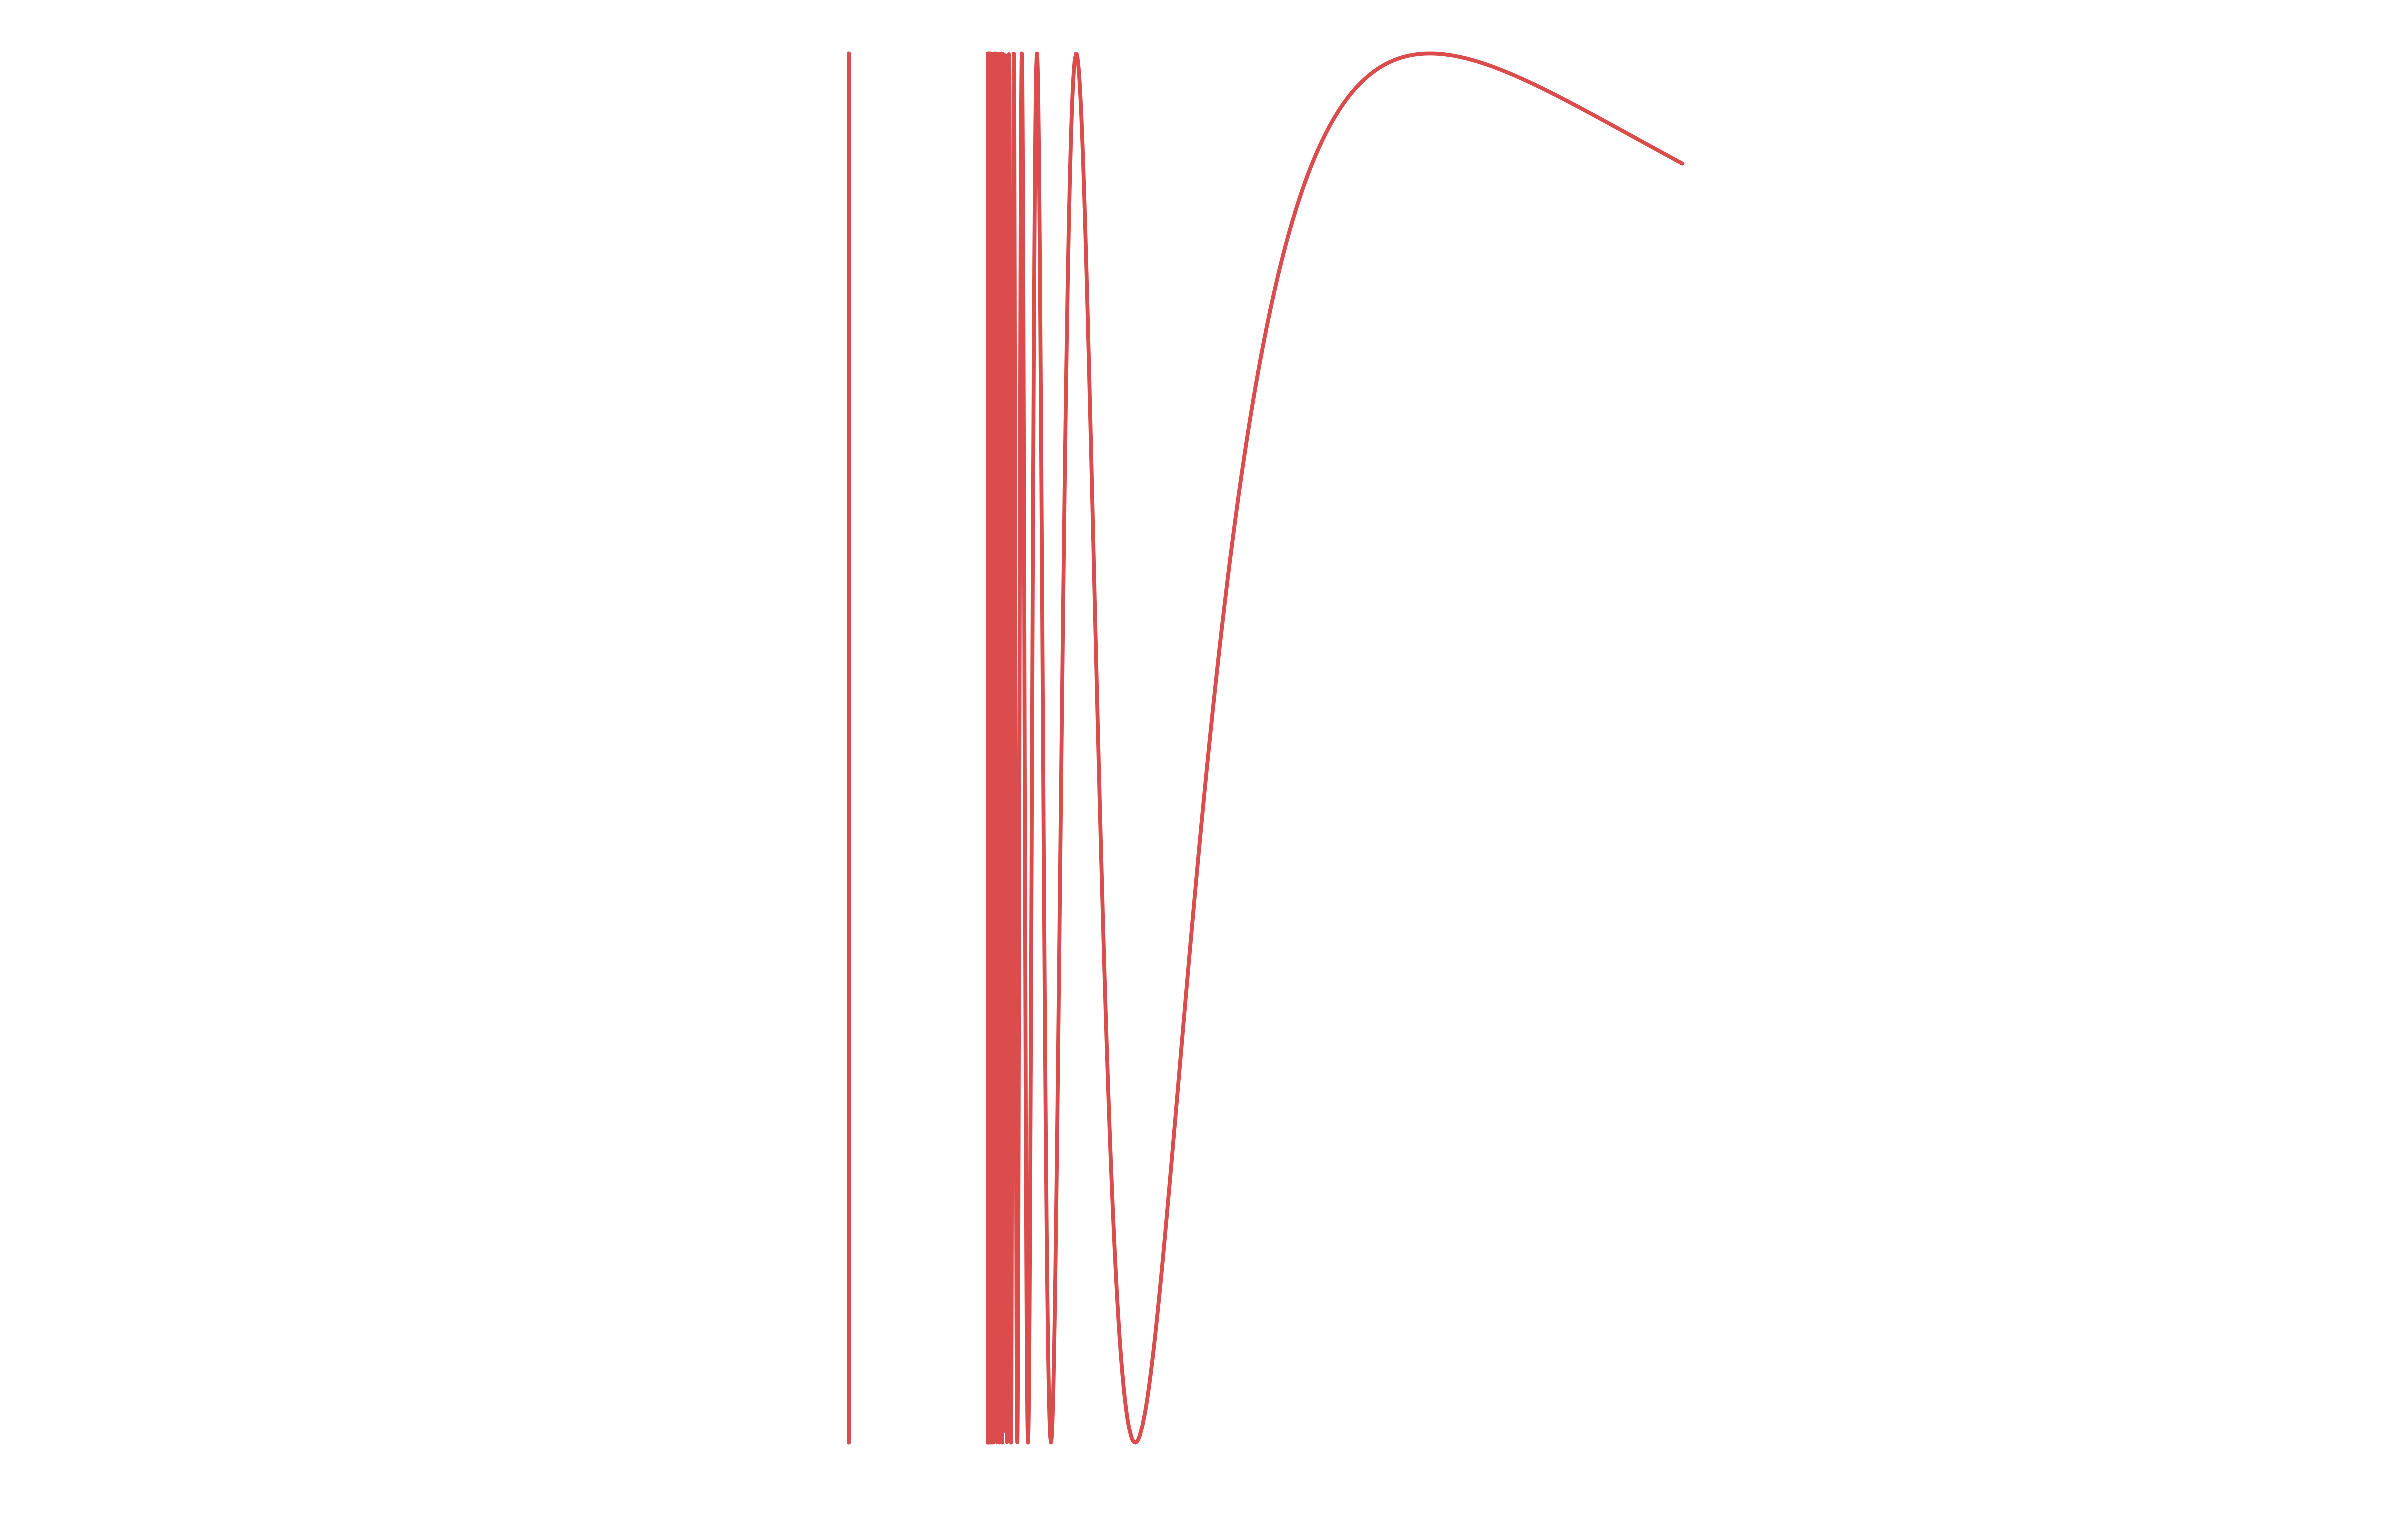
\includegraphics[scale = 0.2]{Figures/Chapter3/topologistsSineCurve.eps}
            \caption{The topologists Sine Curve, defined by $x \times \sin{\frac{1}{x}}$.}
            \label{fig_3.2}
        \end{figure}

        Let $S=\{x \times \sin{\frac{1}{x}}:0 < x \leq 1\}$. This is the image of the continuous map
        $x \rightarrow x \times \sin{\frac{1}{x}$ from $(0,1] \rightarrow \R^2$, Since $(0,1]$ is
            connected, then so is $S$. by theorem \ref{3.1.6}. We call $\cl{S}=S \cup (0 \times
            [-1,1])$ the \textbf{topologist's sine curve} (see figure \ref{fig_3.2}).

            Suppose that $f:[a,c] \rightarrow \cl{S}$ is a path begining at $0$ and ending at a
            point in  $S$. The set  $T=\{t \in \R:f(t) \in 0 \times [-1,1]\}$ is closed, so it has a
            largest element $b$. Then  $f$ is a path mapping  $b \rightarrow 0 \times [-1,1]$ and
            taking all other points to $S$. Suppose that  $[b,c]=[0,1]$ and let $f(t)=(x(t),y(t))$
            where $x(0)=0$, $x(t)>0$ and $y(t)=\sin{\frac{1}{x(t)}}$ for all $t>0$. For  $n \in
            \Z^+$, choose  $0<u<x(\frac{1}{n})$ such that $\sin{\frac{1}{u}}=(-1)^n$. By the
            intermediate value theorem, there are $0<t_n<\frac{1}{n}$ with $x(t_n)=u$. Then the
            sequence $\{t_n\} \rightarrow 0$, and $x(t_n)=(-1)^n$, which diverges; a contradiciton
            since $x(0)=0$ and $\{t_n\} \rightarrow 0$. Hence $\cl{S}$ is not path connected.

    \end{enumerate}
\end{example} 

\section{Outer Measures}

\begin{definition}
    Let $X$ be a set. An \textbf{outer-measure} on $X$ is a function $m^\ast:2^X
    \xrightarrow{} [0, \infty)$ for which the following are true:
    \begin{enumerate}
        \item[(1)] $m^\ast(\emptyset)=0$.

        \item[(2)] If $A \subseteq B$, then $m^\ast(A) \leq m^\ast(B)$.

        \item[(3)] If $\{A_n\}$ is a countable collection of subsets of $X$,
            then
            \begin{equation*}
                m^\ast\Big{(} \bigcup{A_n} \Big{)} \leq \sum{m^\ast(A_n)}
            \end{equation*}
    \end{enumerate}
\end{definition}

\begin{lemma}\label{lemma_1.3.1}
    Let $X$ be a set, and  $\Ec$ a collection of subsets of $X$ for which
    $\emtyset \in \Ec$ and $X \in \Ec$, and let $l:\Ec \xrightarrow{} [0, \infty]$
    a function for which $l(\emptyset)=0$. For any $A \subseteq X$, define
    \begin{equation}\label{equation_1.4}
        m^\ast(A)=\inf{\Big{\{} \sum{l(E_n)} : E_n \in \Ec, \text{ and }
       A \subseteq \bigcup{E_n} \Big{\}}}
    \end{equation}
    Then $m^\ast$ defines an outer-measure.
\end{lemma}
\begin{proof}
    For all $A \subseteq X$, there is a collection $\{E_n\}$ of sets of $\Ec$
    for which $A \subseteq \bigcup{E_n}$. Observe first, that since $l(E_n) \geq
    0$ for all $n$, that  $\sum{l(E_n)} \geq 0$. This makes $m^\ast(A) \geq 0$.
    Now, choose $E_n=\emptyset$ for all  $n$, and we get  $m^\ast(\emptyset)=0$.

    Now, let $A \subseteq B$ subsets of $X$, and let  $\{E_n\}$ a countable
    cover of $B$. Then  $\{E_n\}$ is also a countable cover of $A$. Define then
     $E=\{\sum{l(E_n)} : A \subseteq \bigcup{E_n}\}$ and $F=\{\sum{l(E_n)} :
     B \subseteq \bigcup{E_n}\}$. Since $A \subseteq B$, $F \subseteq E$.
     Therefore, by least upper bounds, we have $\inf{F} \leq \inf{B}$, that is
     $m^\ast(A) \leq m^\ast(B)$.

     Lastly, let $\{A_n\}$ be a countable collection of sets of $X$, and let
     $A=\bigcup{A_n}$. Now, if at least one of the $m(A_n)=\infty$, then we are
     done. Suppose then that $m(A_n)<\infty$ for all $n$. Now, there exists a
     cover of  $A_n$,  $\{E_{n,k}\}_k$ for which
     \begin{equation*}
         \sum_{k}{l(E_{n,k})}<m^\ast(A)+\frac{1}{2^k}
     \end{equation*}
     consider now the countable collection
     $\{E_{n,k}\}_{n,k}=\bigcup_{n}{\{E_{n,k}\}_k}$. Then $\{E_{n,k}\}_{n,k}$ is
     a countable cover for $A$, and we get
     \begin{equation*}
         m^\ast(A) \leq \sum_n{\sum_k{l(E_{n,k})}}<
         \sum_n{m^\ast(A_n)+\frac{1}{2^k}}=\sum_n{m^\ast(A_n)}+\e
     \end{equation*}
     Take then $\e>0$ small, and we get the result.
\end{proof}
\begin{corollary}
    If $E$ is a set of $\Ec$, then $m^\ast(E)=l(E)$.
\end{corollary}
\begin{proof}
    Observe that $E$ covers itself, so that
    $m^\ast(E)=\inf{\{\sum_{i=1}^1{E}\}}=\inf{l(E)}=l(E)$.
\end{proof}

\begin{definition}
    Let $X$ be a set. We call a subset $A$ of  $X$  \textbf{$m^\ast$-measurable}
    if for any subset $E$ of  $X$,
    \begin{equation}\label{equation_1.5}
        m^\ast(E)=m^\ast(E \cap A)+m^\ast(E \cap \com{X}{A})
    \end{equation}
\end{definition}

\begin{lemma}\label{lemma_1.3.2}
    Let $X$ be a set. A subset $A$ of $X$ is  $m^\ast$-measurable if, and only
    if
    \begin{equation*}
        m^\ast(E) \geq m^\ast(E \cap A)+m^\ast(E \cap \com{X}{A}) \text{ for all }
        E \subseteq X
    \end{equation*}
\end{lemma}

\begin{theorem}[Carath\'eodory's Theorem]\label{theorem_1.3.3}
    Let $X$ be a set, and $m^\ast$ an outer-measure on $X$. Then the collection
    of all $m^\ast$-measurable sets forms a  $\s$-algebra. Moreover,  $m^\ast$
    is a complete measure on this $\s$-algebra.
\end{theorem}
\begin{proof}
    Let $\Mc$ be the collection of all  $m^\ast$-measurable sets. Observe first
    that if  $A \in \Mc$, then so is $\com{X}{A}$, by symetry of equation
    \ref{equation_1.5}. So $\Mc$ is closed under complements. Now, let  $A,B \in
    \Mc$. Then we have
    \begin{align*}
        m^\ast(E) &= m^\ast(E \cap A)+m^\ast(E \cap \com{X}{A}) \\
               &= m^\ast(E \cap A \cap B)+m^\ast(E \cap A \cap \com{X}{B})
                        +m^\ast(E \cap B \cap \com{X}{A})+m^\ast(E \cap
                        \com{X}{A} \cap \com{X}{B}) \\
    \end{align*}
    Now, since $A \cup B=(A \cap B) \cup (A \cap \com{X}{B}) \cup (B \cap
    \com{X}{A})$, so by subadditivity, we get
    \begin{equation*}
        m^\ast(E \cap A \cap B)+m^\ast(E \cap A \cap \com{X}{B})+m^\ast(E \cap
        \com{X}{A} \cap B) \geq m^\ast(E \cap (A \cup B))
    \end{equation*}
    i.e. $m^\ast(E) \geq m^\ast(E \cap (A \cup B))+m^\ast(E \cap \com{X}{(A \cup
    B)})$. That is, $A \cup B \in \Mc$, making $\Mc$ an algebra.

    Now, let  $\{A_n\}$ be a countable disjoint collection of
    $m^\ast$-measurable sets, and take  $B_n=\bigcup_{i=1}^n{A_i}$, and take
    $B=\bigcup{B_n}$. Then for all $E \subseteq X$
    \begin{align*}
        m^\ast(E \cap B_n) &= m^\ast(E \cap B_n \cap A_n)+m^\ast(E \cap B_n \cap
                        \com{X}{A_n}) \\
                     &= m^\ast(E \ca A_n)+m^\ast(E \cap B_{n-1})
    \end{align*}
    an induction argument on the collection $\{B_n\}$ gives us
    \begin{equation*}
        m^\ast(E \cap B_n)=\sum_{i=1}^n{m^\ast(E \cap A_i)}
    \end{equation*}
    therefore
    \begin{equation*}
        m^\ast(E)=m^\ast(E \cap B_n)+m^\ast(E \cap \com{X}{B_n}) \geq
        \sum_{i=1}^n{m^\at(E \cap A_i)}+m^\ast(E \cap \com{X}{B_n})
    \end{equation*}
    letting $n \xrightarrow{} \infty$,
    \begin{equation*}
        m^\ast(E) \geq \sum{m^\at(E \cap A_n)}+m^\ast(E \cap \com{X}{B_n})
    \end{equation*}
    so that $B \in \Mc$. Taking $E=B$, we get  $m^\ast(B)=\sum{m^\ast(A_n)}$ so
    that $m^\ast$ is countably additive, and $\Mc$ is a $\s$-algebra.

    Finally, let $m^\ast(A)=0$, then for any $E \subseteq X$, we have
    \begin{equation*}
        m^\ast(E) \leq m^\ast(E \cap A)+m^\ast(E \cap \com{X}{A})=
        m^\ast(E \cap \com{X}{A}) \leq m^\ast(E)
    \end{equation*}
    so that $A \in \Mc$, which makes $m^\ast$ complete on $\Mc$.
\end{proof}

\begin{definition}
    Let $X$ be a set, and  $\Ac$ an algebra on  $X$. We define a
    \textbf{pre-measure} on $\Ac$ to be a function  $m_0:\Ac \xrightarrow{}
    [0,\infty]$ for which
    \begin{enumerate}
        \item[(1)] $m_0(\emptyset)=0$.

        \item[(2)] If $\{A_n\}$ is a countably disjoint collection of sets in
            $\Ac$, for which  $\bigcup{A_n} \in \Ac$, then
            \begin{equation}\label{equation_1.6}
                m_0\Big{(} \bigcup{A_n} \Big{)}=\sum{m_0(A_n)}
            \end{equation}
    \end{enumerate}
\end{definition}

\begin{lemma}\label{lemma_1.3.4}
    Pre-measures on algebras define outer-measures on the overlying sets.
\end{lemma}
\begin{proof}
    Consider the definition of the outer measure $m^\ast$ from equation
    \ref{equation_1.4}, simply take $l=m_0$, and $\Ec=\Ac$.
\end{proof}

\begin{lemma}\label{lemma_1.3.5}
    Let $X$ be a set, and  $\Ac$ an algebra on  $X$. If  $m_0$ is pre-measure on
    $\Ac$, and the measure $m^\ast$ is define by
    \begin{equation*}
        m^\ast(A)=\inf{\Big{\{} \sum{m_0(E_n)} : E_n \in \Ac, \text{ and }
       A \subseteq \bigcup{E_n} \Big{\}}}
    \end{equation*}
    then the following are true.
    \begin{enumerate}
        \item[(1)] $m_0=m^\ast$ on $\Ac$.

        \item[(2)] Every set in $\Ac$ is  $m^\ast$-measurable.
    \end{enumerate}
\end{lemma}
\begin{proof}
    For (1), suppose that $A \in \Ac$, and that $A \subseteq \bigcup{E_n}$ for
    $E_n \in \Ac$. Take
    \begin{equation*}
        F_n=A \cap \com{A_n}{\Big{(} \bigcup_{i=1}^{n-1}{A_i} \Big{)}}
    \end{equation*}
    then $\{F_n\}$ is a disjoint countable collection of sets of $\Ac$ for which
     $A=\bigcup{F_n}$. Hence
     \begin{equation*}
         mo(A)=\sum{m_0(F_n)} \leq \sum{m_0(E_n)}
     \end{equation*}
     it follows from hypothesis that $m_0(A) \leq m^\ast(E)$. For the reverse
     inclusion, simply take $A \subseteq \bigcup{E_n}$ with $A=E_1$ and
     $E_n=\emptyset$ for all  $n>1$.

     For (2), if $A \in \Ac$, and $E \subseteq X$, and $\e>0$, there is a
     collection  $\{B_n\}$ of sets of $\Ac$ with  $A \subseteq \bigcup{B_n}$,
     and
     \begin{equation*}
         \sum{m_0(B_n)}<m^\ast(A)+\e
     \end{equation*}
     by additivity of $m_0$ on $\Ac$, we get
     \begin{equation*}
         m^\ast(E)+\e \geq \sum{m_0(B_n \cap A)}+\sum{m_0(B_n \cap \com{X}{A})}
                    \geq m^\ast(E \cap A)+m^\ast(E \cap \com{X}{A})
     \end{equation*}
\end{proof}

\begin{theorem}\label{theorem_1.3.6}
    Let $X$ be a set, and  $\Ac$ an algerba on  $X$. Let  $m_0$ be a pre-measure
    on $\Ac$, and let  $\Mc$ the  $\s$-algebra generated by  $\Ac$. Then there
    exists a measure  $m$ on  $\Mc$ whose restriction to  $\AC$ is  $m_0$.
    Moreover, if $n$ is another measure extending from $m_0$, then
    \begin{equation*}
        n(E) \leq m(E) \text{ for all } E \in \Mc
    \end{equation*}
    where equality holds when $m(E)<\infty$. Lastly, if $m_0$ is $\s$-finite,
    then  $m$ is the unique extension of  $m_0$ to $\Mc$.
\end{theorem}
\begin{proof}
    Define again,
    \begin{equation*}
        m^\ast(A)=\inf{\Big{\{} \sum{m_0(E_k)} : E_k \in \Ac, \text{ and }
       A \subseteq \bigcup{E_k} \Big{\}}}
    \end{equation*}
    then by Carath\'eodory's theorem, lemma \ref{lemma_1.3.5}, the first result
    follows, since the $\s$-algebra of all  $m^\ast$-measurable sets contains
    $\Ac$, and as consequence, also contains $\Mc$.

    Now, let $E \in \Mc$ with $E \subseteq \bigcup{A_k}$, where $A_k \in \Ac$.
    Then
    \begin{equation*}
        n(E) \leq \sum{n(A_n)}=\sum{m_0(A_n)}
    \end{equation*}
    which gives us $n(E) \leq m(E)$. Now, set $A=\bigcup{A_n}$, and observe that
    \begin{equation*}
        n(A)=\lim_{k \xrightarrow{} \infty}{n\Big{(} \bigcup_{i=1}^k{A_i} \Big{)}}
        =\lim_{k \xrightarrow{} \infty}{m\Big{(} \bigcup_{i=1}^k{A_i}
        \Big{)}}=m(A)
    \end{equation*}
    if $m(E)<\infty$, choose $A_k$ such that  $m(A)<m(E)+\e$ for $\e>0$. Then
    $m(\com{A}{E})<\e$, and
    \begin{equation*}
        m(E) \leq m(A)=n(A)=n(E)+n(\com{A}{E}) \leq n(E)+m(\com{A}{E}) \leq
        n(E)+\e
    \end{equation*}
    taking $\e$ small, we get $n(E)=m(E)$.

    Finally, suppose that $m_0$ is $\s$-finite, and let $X=\bigcup{A_k}$ for
    s me0disjoint collection $\ A_n\}$, then $ m_0 m_0)<\infty$. Then for every
    $E \in \Mc$,
    \begin{equation*}
        m(E)=\sum{m(E \cap A_k)}=\sum{n(E \cap A_k)}=n(E)
    \end{equation*}
    so that $m=n$, making $m$ unique.
\end{proof}

\section{Roots of Analytic Functions}

%----------------------------------------------------------------------------------------
%	SECTION 1.1
%----------------------------------------------------------------------------------------

\section{Rectifiable Curves.}

\begin{definition}
    We call a continuous mapping $\gamma:[a,b] \rightarrow \R^k$ a
    \textbf{curve} in $\R^k$, on  an interval $[a,b]$. If  $\gamma$ is 1-1, we
    call the curve an \textbf{arc}, and we call  $\gamma$ a \textbf{closed
    curve} if  $\gamma(a)=\gamma(b)$.

    Now, for each partition $P$ of  $[a,b]$, and for  $\gamma$ a curve on
    $[a,b]$, and let:
        \begin{equation}
            \Lambda(\gamma,P)=\sum_{i=1}^{n}{||\gamma(x_i)-\gamma(x_{i-1})||}		
        \end{equation}
    We deefine the \textbf{length} of $\gamma$ to be :
        \begin{equation}
            \Lambda(\gamma)=\sup_{P}{\Lambda(\gamma,P)}		
        \end{equation} 
        If $\gamma$ is of finite length  (i.e. $\Lambda(\gamma)<\infty$), then
        we call $\gamma$ a \textbf{rectifiable} curve.
\end{definition}

\begin{theorem}\label{7.5.1}
    Let $\gamma$ be a differentiable curve on  $[a,b]$, if  $\gamma'$ is
    continuous, then  $\gamma$ is rectifiable and
        \begin{equation}
            \Lambda(\gamma)=\int_{a}^{b}{||\gamma'|| dt}		
        \end{equation} 
\end{theorem}
\begin{proof}
    If $a \leq x_{i-1}<x_i \leq b$, then
    $||\gamma(x_i)-\gamma(x_{i-1})||=||\int_{x_{i-1}}^{x_i}{\gamma' dt}|| \leq
    \int_{x_{i-1}}^{x_i}{||\gamma'|| dt}$, by the Fundamental theorem of
    calculus, thus $\Lambda(\gamma,P) \leq \int_{a}^{b}{||\gamma'|| dt}$ 
    for every partition $P$ of  $[a,b]$, then cinsequently, we have
    $\Lambda(\gamma)=\int{||\gamma'|| dt}$. Consequently, $\gamma$ is
    rectifiable.

    Now let  $\epsilon>0$, since  $\gamma'$ is uniformly continuous on  $[a,b]$,
    there is a  $\delta>0$ such that  $||\gamma'(s)-\gamma'(t)||<\epsilon$
    whenever  $|s-y|<\delta$ for  $s,t \in [a,b]$. Let $P$ be a partition of
    $[a,b]$, with  $\Delta{x_i}<\delta$ for all  $i$, and it  $x_{i-1} \leq t
    \leq x_i$, we have  $||\gamma'(t)|| \leq ||\gamma'(x_i)||+\epsilon$, hence:
        \begin{align*}
            \int_{x_{i-1}}^{x_i}{||\gamma'||\Delta{x_i}} &\leq ||\gamma'(x_i)||\Delta{x_i}+\epsilon\Delta{x_i} \\ 
                &= ||\int_{x_{i-1}}^{x_i}{(\gamma'(t)+\gamma'(x_i)-\gamma'(t))}||+\epsilon\Delta{x_i} \\
                &\leq ||\int_{x_{i-1}}^{x_i}{\gamma' dt}||+||\int_{x_{i-1}}^{x_i}{(\gamma'(x_i)-\gamma'(t)) dt}||+\epsilon\Delta{x_i} \\
                & \leq ||\gamma(x_i)-\gamma(x_{i-1})||+2\epsilon\Delta{x_i} \\
        \end{align*}
    Thus, $\int_{a}^{b}{||\gamma'|| dt} \leq \Lambda(\gamma,P)+2\epsilon(b-a)$, 
    so for  $\epsilon$ small enough, we get that  $\int{||\gamma'||} \leq \Lambda(\gamma)$.
\end{proof}

\section{Gr\"obner Bases}
\label{section_7.6}

\begin{definition}
  Let $R$ be a Noetherian ring, and $\leq$ a monomial ordering on
  $R[x_1, \dots, x_n]$. We define the \textbf{leading term} of a
  polynomial $f(x_1, \dots, x_n)$ to be the maximum element of the
  ideal $(f)$, and denote it $LT(f)$. If $\af$ is an ideal in $R[x_1,
  \dots, x_n]$, then we define the \textbf{ideal of leading terms} of
  $\af$ to be the ideal generated by all leading terms of polynomials
  of $\af$; i.e.
  \begin{equation*}
    LT(\af)=(LT(f) : f \in \af)
  \end{equation*}
  If $\af=(f_1, \dots, f_m)$, we write $LT(f_1, \dots, f_m)$. If
  $\af=(f)$, we keep the previous convention $LT(\af)$.
\end{definition}

\begin{definition}
  Let $f(x_1, \dots, x_n)$ a multi-variate polynomial over a
  Noetherian ring. We define the \textbf{multi-degree} of $f$ to be
  the multi-degree of $LT(f)$, and we denote it $\partial{f}$.
\end{definition}

\begin{proposition}\label{proposition_7.6.1}
  Let $f_1, \dots, f_m$ be multivariate polynomials over a Noetherian
  ring. Then
  \begin{equation*}
    (LT(f_1), \dots, LT(f_m)) \subseteq LT(f_1, \dots, f_m)
  \end{equation*}
\end{proposition}
\begin{proof}
  Observe that since $f_i \in \af$ for each $1 \leq i \leq m$, then
  $LT(f_i) \in LT(\af)$ for each $1 \leq i \leq m$.
\end{proof}

\begin{proposition}\label{proposition_7.6.2}
  Let $k$ be field, and $f,g \in k[x_1, \dots, x_n]$. Then
  the following are true:
  \begin{enumerate}
    \item[(1)] $LT(fg)=LT(f)LT(g)$.

    \item[(2)] $LT(f+g) \leq \max{\{LT(f), LT(g)\}}$ with equality
      holding if $LT(f) \neq LT(g)$.
  \end{enumerate}
\end{proposition}
\begin{proof}
  Let $AX^\a=LT(f)$ and $BX^\b=LT(g)$, and make the convention $f(x_1,
  \dots, x_n)=f(X)$. Then we have for some $h,h' \in R[x_1, \dots,
  x_n]$ that $f(X)=AX^\a+h(X)$ and $g=BX^\b+h'(X)$. Then
  \begin{align*}
    fg(X) &=  (AX^\a+h(X))(BX^\b+h'(X))  \\
          &= (AB)X^\a X^\b+(AX^\a h'(X)+BX^\b h(X)+h(X)h'(X))  \\
          &=  (AB)X^{\a+\b}+h''(X)  \\
  \end{align*}
  so that $LT(fg)=LT(f)LT(g)$.

  Now, we also observe that
  \begin{equation*}
    f+g(X)=(AX^\a+BX^\b)+(h(X)+h'(X))
  \end{equation*}
  if $\a=\b$, and $B=-A$, then $f+g(X)=h(X)+h'(X)$ and $LT(f+g)<AX^\a$
  and $LT(f+g)<BX^\b$, so that $LT(f+g)<\max{\{AX^\a,BX^\b\}}$. Now, we have
  if  $\a \neq \b$, then
  \begin{align*}
    f+g(X)=AX^\a+(BX^\b+h(X)+h'(X))  & \text{ if } \b < \a  \\
    f+g(X)=AX^\b+(BX^\a+h(X)+h'(X))  & \text{ if } \a < \b  \\
  \end{align*}
  in either case either $LT(f+g)=\max{\{X^\a,X^\b\}}$.
\end{proof}
\begin{corollary}
  The following are true:
  \begin{enumerate}
    \item[(1)] $\partial{(fg)}=\partial{f}+\partial{g}$.

    \item[(2)] $\partial{(f+g)} \leq \max{\{\partial{f},
      \partial{g}\}}$, with equality holding if $\partial{f} \neq
      \partial{g}$.
  \end{enumerate}
\end{corollary}

\begin{proposition}\label{proposition_7.6.3}
  Let $R$ be a Noetherian ring. Let $\af=(X^{\a_1}, \dots, X^{\a_m})$ in $R[x_1,
  \dots x_n]$ and ideal and $f \in R[x_1, \dots, x_n]$. Then $f \in
  \af$ if, and only if each monomial term of $f$ is a multiple of some
  monomial  $X^\a_i$ generating $\af$.
\end{proposition}
\begin{proof}
  Suppose that $f \in \af$. Then
  \begin{equation*}
    f(x_1, \dots, x_n)=f(X)=\sum_{i=1}^m{A_mX^{\a_i}}
  \end{equation*}
  and notice that each monomial $X^{\a_i}$ is a multiple of itself.

  Conversely suppose that
  \begin{equation*}
    f(X)=\sum_{j=1}^n{A_jX^{\b_j}}
  \end{equation*}
  and that there is an $X^{\a_i}$ for which $X^{\a_i}|X^{\b_j}$ for
  all $1 \leq j \leq n$. Then $X^{\b_j} \in (X^{\a_i}) \subseteq
  (X^{\a_1}, \dots, X^{\a_m})$. Then $f \in \af$.
\end{proof}

\begin{example}\label{example_7.8}
  Let $k$ be a field.
  \begin{enumerate}
    \item[(1)] Choose the lexicographic order $x>y$ on $k[x,y]$. Let
      $f(x,y)=x^3y-xy^2+1$ and $g(x,y)=-y^3+x^2y^2-1$. Then
      $LT(f)=x^3y$ with $\partial{f}=(3,1)$, and $LT(g)=x^2y^2$ with
      $\partial{g}=(2,2)$. Then
      \begin{align*}
        LT(fg)=x^5y^3 & \text{ and } \partial{(fg)}=(5,3) \\
        LT(f+g)=x^3y  & \text{ and } \partial{(f+g)}=(3,0)  \\
      \end{align*}
      Now, take $\af=(f,g)$, then $(x^3y,x^2y^2) \subseteq LT(f,g)$.
      However, observe that $yf(x,y)-xg(x,y)=x+y \in \af$, and
      $LT(yf+xg)=x \in LT(f,g)$. However $x \notin
      (x^3y,x^2y^2)$. That is, in general, if $\af=(f_1,
      \dots, f_m)$, then $LT(f_1, \dots, f_m) \neq (LT(f_1), \dots
      LT(f_m))$.

    \item[(2)] Choose the lexicographic ordering $y>x$ in  $k[x,y]$.
      Let again $f(x,y)=x^3y-xy^2+1$ and $g(x,y)=-y^3+x^2y^2-1$. Then
      $LT(f)=xy^2$ with $\partial{f}=(1,2)$ and $LT(g)=y^3$ with
      $\partial{g}=(0,3)$. Then
      \begin{align*}
        LT(fg)=xy^5 & \text{ and } \partial{(fg)}=(1,5) \\
        LT(f+g)=-y^3 & \text{ and } \partial{(f+g)}=(03) \\
      \end{align*}
      Again, we have $(xy^2, y^3) \subseteq LT(f,g)$, but $LT(f,g)
      \neq (xy^2,y^3)$. We observe that $y \in LT(f,g)$ but $y \notin
      (xy^2,y^3)$.

    \item[(3)] Choose any order on $k[x,y]$, and let $f(x,y) \neq 0$.
      Let $\af=(f)$, then $LT(\af)=(LT(f))$, since every monomial term
      of $f$ is a multiple of  $LT(f)$.
  \end{enumerate}
\end{example}

\begin{definition}
  Let $k$ be a field, and $\af$ an ideal of $k[x_1, \dots, x_n]$. We
  call a finite set of generators $G=\{g_1, \dots, g_m\}$ of $\af$ a
  \textbf{Gr\"obner basis} for $\af$ if
  \begin{equation*}
    LT(\af)=(LT(g_1), \dots, LT(g_m))
  \end{equation*}
\end{definition}

\section{Cyclotomic Polynomials}
\label{section_8.7}

\begin{definition}
  We define \textbf{Euler's totient} to be the map $\phi:\Z \xrightarrow{} \Z$
  defined by the rule $\phi(n)=|\{a \in \Z : (a,n)=1\}|$. That is, $\phi$
  of  $n$ is the number of all integers less than  $n$, coprime to  $n$.
\end{definition}

\begin{definition}
  We define $\Xi_n$ to be the \textbf{group of all primitive $n$-th roots of
  unity}, $\xi$ for which  $\xi^n=1$.
\end{definition}

\begin{lemma}\label{lemma_8.7.1}
  $\Xi_n \simeq \faktor{\Z}{n\Z}$.
\end{lemma}
\begin{proof}
  The map $a \xrightarrow{} \xi^a$ defines the required isomorphism.
\end{proof}
\begin{corollary}
  $\ord{\Xi_n}=\phi(n)$ where $\phi$ is Euler's totient.
\end{corollary}
\begin{proof}
  Since $\xi^n \equiv \xi^{0 \mod{n}} \equiv 1$, we have every non identity
  power of $\xi$ has exponenct coprime to  $n$. That is there are $\phi(n)$
  such distinct powers of$\xi$.
\end{proof}
\begin{corollary}
  If $d|n$, then  $\Xi_d \leq \Xi_n$.
\end{corollary}
\begin{proof}
  Notice that if $d|n$, then $d=mn$ for some  $m \in \Z^+$. Then $\xi^d=1$
  implies  $(\xi^d)=\xi^{dm}=\xi^n=1$.
\end{proof}

\begin{definition}
  We define the \textbf{$n$-th cyclotomic polynomial} to be the polynomial
  \begin{equation*}
    \Phi_n(x)=\prod{x-\xi}
  \end{equation*}
  having as roots all $n$-primitive roots of unity.
\end{definition}

\begin{lemma}\label{lemma_8.7.2}
  The $n$-th cyclotomic polynomial  $\Phi_n$ has degree
  $\deg{\Phi_n}=\phi(n)$, where $\phi$ is Euler's totient.
\end{lemma}
\begin{proof}
  Recall that $\ord{\Xi_n}=\phi(n)$, and since the elements of $\Xi_n$ are the
  roots of  $\Phi_n$, there are  $\phi(n)$ such roots. This puts
  $\deg{\Phi_n}=\phi(n)$.
\end{proof}

\begin{example}[Computing Cyclotomic Polynomials]\label{8.18}
  Recall that the polynomial $x^n-1$ has as roots precisely all  $n$-th roots
  of unity  $\xi$, that is $\xi^n=1$. If $x^n-1 \in F[x]$, $F$ a field, the
  the splitting field of  $x^n-1$ is  $F(\xi)$. Then we have
  \begin{equation*}
    x^n-1=\prod_{\xi \in \Xi_n}{(x-\xi)}
  \end{equation*}
  Now, grouping those factors where $\xi^d=1$ for some  $d|n$, then we have
  \begin{equation*}
    x^n-1=\prod_{\xi \in \Xi_d}{(x-\xi)}\prod_{\xi \in \Xi_n}{(x-\xi)}=
    \prod{d|n}{\prod_{\xi \in \Xi_n}{(x-\xi)}}=\prod_{d|n}{\Phi_n(x)}
  \end{equation*}
  that is,
  \begin{equation*}
    x^n-1=\prod_{d|n}{\Phi_d(x)}
  \end{equation*}
  which gives a method for computing $\Phi_n$ recursively.

  We have  $\Phi_1(x)=x-1$ and $\Phi_2(x)=x+1$. Now,
  $\Phi_3(x)=\Phi_1(x)\Phi_3(x)=(x-1)\Phi_3(x)$, so that
  \begin{equation*}
    Phi_n(x)=x^2+x+1
  \end{equation*}
  We have
  $\Phi_4(x)=\Phi_1(x)\Phi_2(x)\Phi_4(x)=(x-1)(x+1)\Phi_4(x)=(x^2-1)\Phi_4(x)$.
  So
  \begin{equation*}
    \Phi_4(x)=x^2+1
  \end{equation*}
  Similarly,
  \begin{align*}
    \Phi_5(x)   &=  x^4+x^3+x+1 \\
    \Phi_6(x)   &=  x^2-x+1 \\
    \Phi_7(x)   &=  x^6+x^5+x^4+x^3+x^2+x+1 \\
    \Phi_8(x)   &= x^4+1    \\
    \Phi_9(x)   &=  x^6+x^x+1   \\
    \Phi_{10}(x)   &=   x^4-x^3+x^2-x+1 \\
    \Phi_{11}(x)   &=   x^{10}+x^9+x^8+x^7+x^6+x^5+x^4+x^3+x^2+x+1  \\
    \Phi_{12}(x)   &=   x^4-x^2+1   \\
  \end{align*}
  Also observe that if $p$ is prime, then
  \begin{equation*}
    \Phi_p(x)=\sum_{i=0}^{p-1}{x^i}=x^{p-1}+x^p+\dots+x+1
  \end{equation*}
\end{example}

\begin{lemma}\label{lemma_8.7.3}
  $\Phi_n(x)$ is monic over $\Z$.
\end{lemma}
\begin{proof}
  Notice that since $x^n-1=\prod{\Phi_d(x)}$, is monic, then each $\Phi_d$
  must also be monic for all  $d|n$.

  Now, by induction on $n$, for  $n=1$, it is clear that  $x-1$ has
  coefficiencts in  $\Z$  (if $x^n-1 \in \Z[x]$ we are done, if not, just take
  $1_F \xrightarrow{} 1_\Z$, whre $F$ is the underlying field of  $x^n-1$).
  Now, suppose that $\Phi_d(x) \in \Z[x]$ for all $1 \leq d <n$, and  $d|n$.
  Then  $x^n-1=f(x)\Phi_n(x)$, where $f(x)=\prod{\Phi_d(x)}$ is monic over
  $\Z$. Moreover,  $f|x^n-1$, in the splitting field $\Q(\xi)$ (since we take
  $1_F \xrightarrow{} F_\Z$), where $\xi^n=1$. Then  $f|x^n-1$ over  $\Q$ by
  the division theorem, and by Gauss' lemma, $f|x^n-1$ in $\Z$. So $\Phi_n \in
  \Z[x]$.
\end{proof}

\begin{theorem}\label{lemma_8.7.4}
  $\Phi_n$ is irreducible over  $\Z$.
\end{theorem}
\begin{proof}
  Again, if $x^n-1 \in F[x]$ for some field $F$, take  $1_F \xrightarrow{}
  1_\Z$ so that $x^n-1 \in \Z[x]$. Suppose then that $\Phi_n(x)=f(x)g(x)$
  where $f$ and  $g$ are monic, and  $f$ is irreducible. Let $\xi^n=1$, a
  primitive $n$-th root, so that $\xi$ is a root of $f$. Then $f$ is the
  minimal polynomial for $\xi$ over  $\Q$. Now, let $p$ a prime such that $p
  \nmid n$. Then $\xi^p$ is a $n$-th root, of $f$ or $g$. If  $f(\xi^p)=0$,
  then for all $a$ with  $(a,n)=1$, we have $\xi^a$ is a root of $f$.
  Moreover,  $a=p_1 \dots p_k$ where each $p_i \nmid n$ is prime. That means
  tht  $\xi^{p_1}$, $(\xi^{p_1})^{p_2}, \dots, \xi^n$ are all roots of $f$
  making  $f=\Phi_n$ and we are done.

  Suppose then that $g(\xi^p)=0$. Then $\xi$ is root of  $g(x^p)$,
  and since $f$ is minimal, $f|g(x^p)$ in $\Z[x]$. Then we have
  $g(x^p)=f(x)h(x)$ for $f,h \in \Z[x]$. reducing mod $p$, we get
  $g(x^p) \equiv f(x)h(x) \mod{p}$ in $\F_p[x]$; but $g(x^p) \equiv (g(x))^p
  \mod{p}$. Since $\F_p[x]$ is a unique factorization domain, we get that $f
  \mod{p}$ and $g \mod{p}$ have a common factor. Then $\Phi_n(x) \equiv
  f(x)g(x) \mod{p}$ has a multiple root in $\F_p[x]$ ; implying that $x^n-1$
  has a multiple root, which is impossible; since $x^n-1$ has  $n$ distinct
  roots. Therefore $\xi^p$ is a root of  $f$.
\end{proof}
\begin{corollary}
  $[\Q(\xi):\Q]=\phi(n)$.
\end{corollary}
\begin{proof}
  We have by above that $\Phi_n$ is the minimal polynomial for  $\xi$ over
  $\Q$.
\end{proof}

\begin{example}\label{8.19}
  Let $\xi^8=1$ an  $8$-th root of unity. Then  $[\Q(\xi):\Q]=4$ and $\Q(\xi)$
  has minimal polynomial $\Phi_8(x)=x^4+1$. Moreover, $\Q(\xi)$ contains a
  primitive $4$-th root of unity $i^4=1$ (over $\C$,  $i^2=-1$). So that
  $\Q(i) \subseteq \Q(\xi)$. We als get that $\xi+\xi^7=\sqrt[]{2}$ (since
  $\xi=e^{\frac{2i\pi}{8}}$ over $\C$), and $\Q(\xi)=\Q(i,\sqrt[]{2})$.
\end{example}



\nocite{*}

\bibliography{references.bib}
\bibliographystyle{ieeetr}

\end{document}
